\documentclass[bibtotoc,liststotoc,BCOR5mm,DIV12]{scrbook}

% use this declaration to set specific page margins
%\usepackage[a4paper , lmargin = {2.7cm} , rmargin = {2.9cm} , tmargin = {2.7cm} , bmargin = {4.6cm} ]{geometry}
\usepackage[a4paper]{geometry}

\usepackage[german, english]{babel}
\usepackage{bibgerm}       		% german references
\usepackage[latin1]{inputenc} % german characters
\usepackage{graphicx} 				% it's recommended to use PDF images but you can use JPG or PNG as well
\usepackage{url}           		% format URLs
\usepackage{hyperref} 				% create hyperlinks
\usepackage{listings, color}	% for source code
\usepackage{subfig}						% two figures next to each other (example: figure 3a), figure 3b)
\usepackage{scrpage2}					% header and footer line


\typeout{pdfcompresslevel=\the\pdfcompresslevel}
\typeout{pdfobjcompresslevel=\the\pdfobjcompresslevel}
\typeout{pdfminorversion=\the\pdfminorversion}



\newtheorem{definition}{Conjecture}[section]
 

 
\DeclareMathAlphabet{\mathpzc}{OT1}{pzc}{m}{it}

	
\usepackage{csquotes}




% header and footer line - no header & footer line on pages where a new chapter starts
\pagestyle{scrheadings}
\ohead{Semantic Blockchain}
\ihead{S. Matthew English}
\ofoot[]{\thepage}
\ifoot{MSc Thesis, Universit{\"a}t Bonn, Enterprise Information Systems (EIS), 2016}




% set path where images are stored
\graphicspath{{./img/}}

%
% der Befehl \hypenation versteht keine Sonderzeichen, also weder �
% noch "a noch \"a. W�rter die derartige Zeichen enthalten m�ssen
% direkt im Text getrennt werden, z.B. W�r\-ter
%
\hyphenation{te-le-com-muni-cation 
te-le-com-muni-cation-specific 
Te-le-kom-mu-ni-ka-tions-API} 					% use this file to set explicit hyphenations (doesn't seem to work correctly)

\begin{document}
% ---------------------------------------------------------------
\frontmatter
    \thispagestyle{empty}
\begin{center}

\vspace*{1.4cm}
{\LARGE \textbf{Rheinische Friedrich-Wilhelms-Universit{\"a}t Bonn}}

\vspace{0.5cm}

{\large Enterprise Information Systems (EIS)\\[1mm]}
{\large Institute for Applied Computer Science\\[5mm]}

Regina-Pacis-Weg 3\\
53113 Bonn\\
Federal Republic of Germany\\
www.eis.iai.uni-bonn.de\\

\vspace*{1cm}


\includegraphics[width=4cm]{bonn.png}

\vspace*{1.0cm}

{\LARGE MSc. Thesis}\\

\vspace{1.0cm}
{\LARGE \textbf{Semantic Blockchain:}}\\
\vspace*{0.3cm}
{\LARGE \textbf{Analytical Assessment of Productive Symbioses}}\\
\vspace*{1.0cm}
{\LARGE S. Matthew English}
\\
\vspace*{0.5cm}
Matriculation Number: 2908245\\
31.10.2016\\ % 	date of submission
\vspace*{1.0cm}

Supervised by\\
Prof. Dr. S{\"o}ren Auer\\
\vspace*{0.5cm}
Co-Examiner\\
Prof. Dr. Jens Lehmann
\vspace{3cm}



\end{center}


   	% \thispagestyle{empty}
    % \cleardoublepage
    
    \thispagestyle{empty}
\vspace*{3cm}


\begin{center}

\includegraphics[width=0.4\textwidth]{fraunhofer.jpg}
\end{center}

\vspace*{0.2cm}

\begin{center}
Fraunhofer Institut f{\"u}r Intelligente Analyse und Informationssysteme (IAIS)\\
Schloss Birlinghoven\\
53757 Sankt Augustin, Germany\\
\end{center}
\vspace*{0.5cm}

% \noindent This dissertation originated in cooperation with the Fraunhofer Institut f{\"u}r Intelligente Analyse und Informationssysteme (IAIS).

% \vspace*{1cm}
% \noindent 
% First of all I would like to thank  at the Fraunhofer IAIS & the Universit{\"a}t Bonn for giving me the opportunity to carry out state of the art research in this field. 
% \\
% \\
% Special thanks to all members of the Bitcoin MeetUp in K{\"o}ln for their invaluable assistance.
% Additionally I would like to recognize H{\'e}ctor Ugarte, etc...
% \\
% \\
% Furthermore I would like to thank my girlfrind Yulia, and of course my wonderful friends and family.  
\noindent{}My task in this work has been to investigate an individual technological system, and in the doing of it nuances of such a degree have been revealed, that my efforts to grasp them in their entirety has consequently meant only a superficial orientation toward those paths, the opening and exploration of which will hopefully crown the work of future endeavours with success. \\

\noindent{}I am not sympathetic towards the attitude which favors the repression of certain potential working hypotheses because they are possibly erroneous, and so may possess no enduring value.
Certainly I take precautions to guard myself from error, which might indeed become particularly hazardous upon the dizzy heights. I am entirely aware of the risks of such explorations. 
Nevertheless, I do not consider scientific work as a dogmatic contest, but rather as an initiative undertaken for the increase and deepening of knowledge.\\

\noindent{}This contribution is addressed to those who share similar ideas regarding science. \\

\noindent{}In conclusion, I must render thanks to all who have assisted my exertions with valuable aid, especially my dear family, my friends, and Prof. Dr. S{\"o}ren Auer to whose unbiased assistance I am deeply indebted.\\
\vspace*{0.5cm}
\noindent{}\\S. Matthew English\\
\vspace*{0.25cm}
\noindent{}\\Bonn, 2016
    % \thispagestyle{empty}
    % \cleardoublepage
    
    \newpage

\thispagestyle{empty}

\begin{large}

\vspace*{6cm}

\noindent
Hereby I declare that I wrote this thesis myself with the help of no more than the mentioned literature.
\vspace{2cm}

\noindent
Bonn, 31.10.2016

\vspace{3cm}

\hspace*{7cm}%
\dotfill\\
\hspace*{8.5cm}%
\textit{S. Matthew English}

\end{large}
 
    % \thispagestyle{empty}
    % \cleardoublepage
    
    
    \thispagestyle{empty}
\vspace*{1.0cm}

\begin{center}
    \textbf{Abstract}
\end{center}

\vspace*{0.5cm}

\noindent

This work presents a compendium of exploratory analyses on the question of possible use cases for the data structure and incentive mechanisms that together form the foundation for the cryptocurrency Bitcoin. 
The contributions are manifold. 
The first of which is a study in the potential for symbioses between principles of linked open data and that of the design principles inherent in the Bitcoin protocol, concluding with an assessment of the primary vectors for mutual amelioration.
Subsequently we detail the motivation and implementation of a ``smart-contract'' programme for blockchain-based certification of academic credentials.
What follows is a proposal for the disintermediation of inter-cryptocurency exchange that adheres to linked open data principles and hastens the coming inter-linked network of disparate blockchains. 
As Bitcoin remains essentially the world's only truly successful blockchain application we present a detailed analysis of the structural characteristics of the Bitcoin blockchain transaction network, specifically in a time of high value fluctuation and extreme volatility. 
Finally we detail a potential framework for the application of Bitcoin design principles to supply chain management. 
Bitcoin and it's associated protocol remain a fertile research frontier. 
The fundamental motivation for the efforts herein described has been to advance understanding of the techniques Bitcoin technology has pioneered and locate them within a broader framework of scientific knowledge.
    % \thispagestyle{empty}
    % \cleardoublepage
    
    % \thispagestyle{empty}
\vspace*{0.2cm}

\begin{center}
    \textbf{Zusammenfassung}
\end{center}

\vspace*{0.2cm}

\noindent 

    % \thispagestyle{empty}
    
    
    \tableofcontents
    % \cleardoublepage
    % \thispagestyle{empty}
    
    \listoffigures
    % \thispagestyle{empty}
    
    % \listoftables
    % \thispagestyle{empty}
    
% --------------------------------------------------------------

\mainmatter % comment single chapters for faster compilation

    \chapter{Introduction\label{cha:chapter1}}

Bitcoin is an emergent phenomenon realized through the subtle interaction of multiple data structures and incentive mechanisms. 
In isolation the various components that comprise the Bitcoin protocol are well known and in some cases have existed for years.
The novelty of Bitcoin was to combine these elements in a previously unimagined way. 
The success of Bitcoin as a cryptocurrency has generated interest in the design principles employed to realize the system.
This in turn has prompted some to critically reassess traditional methods used to process information. 
The purpose being to determine the extent to which architectural aspects of Bitcoin might be replicated in analogous scenarios to reduce or eliminate current inefficiencies. 

\subsection*{What is ``Semantic Blockchain''?}

Semantic Blockchain is an emerging paradigm in database design and development. 
It describes a model of information repository that incorporates the distributed consensus mechanism popularized by cryptocurrency implementations, such as Bitcoin, and the exchange protocols of the linked open data specification. 
Applications are constructed to support semantic queries and elements of logical reasoning. 
Semantic blockchain principles are integral to the web of interlinked blockchains and the associated features, such as decentralized exchange.

\section{Emergence of Semantic Blockchain}

Bitcoin core developer Jeff Garzik among others has proffered a vision of the Blockchain development phase now underway, in which he described ``a mesh network of cross-chain smart contracts''.
To those familiar with the ideas of the Semantic Web and the global ecosystem of Linked Data this concept should sound startlingly familiar.

\subsection*{Initial Tremors}

The Semantic Web of Linked Data was supposed to transform the Web from a distributed file system into a distributed database system. 
But way back in 2006, Sir Tim Berners-Lee, the man credited with the WWW conception, said that the vision of the Semantic Web was ``largely unrealized''.
For many this proclamation definitively sounded the death knell on an ambitious area of research. 
Google trends is an easy mechanism for confirming this dismal state of affairs, and it seems safe that the notion of the ``\textit{Semantic Web}'' can now take up its mantle in the dustbin of history.

\begin{figure}[!ht]
  \centering
    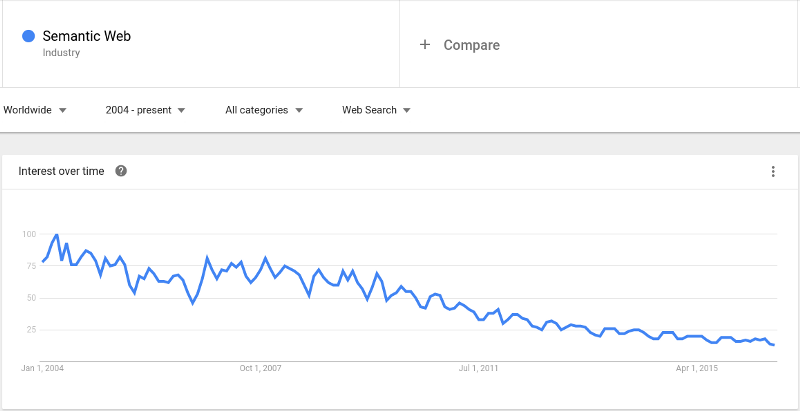
\includegraphics[width=0.5\textwidth]{trends}
  \caption{Google trends result of ``\textit{Semantic Web}'' query.}
\end{figure}

But in our haste to disregard this formerly compelling avenue of exploration we might do well to remember Lazarus or Napoleon, or, for that matter, the once completely infeasible notion of digital money. ``You never step in the same river twice'', said Heraclitus, but some dead ideas have an uncanny way of them of coming back with a vengeance.

\subsection*{Renaissance of Semantics}

The dark ages describe an era of European history wherein much of the culture and civilization established under the Roman Empire was forgotten or disregarded until the epoch we know of as the Renaissance. 
The latest and greatest trend in Artificial Intelligence is Deep Learning which was responsible for the recent victory (or defeat, depending on your perspective) in the struggle of Machine vs. Man over the game of Go. 
The aficionados of ``Deep Learning'' are aware of the Dark Ages into which Neural Networks research was plunged by the highly critical \textit{Perceptrons: An Introduction to Computational Geometry} by Minsky \& Papert, a work which did much to precipitate a 20-year freeze on exploration. 
The same story is familiar to those who have spent any time studying the development of digital money and the ill-fated attempts of the 1990's at its realization. 
In 2008, finally there came the fusion of existing disparate frameworks in a novel way which enabled the creation of Bitcoin, giving rise to the Blockchain as a useful data structure.

\subsection*{Unbalkanizing the Blockchain}

The interchange of homogeneous data facilitated by Blockchain technologies, a new framework for information (value) transmission, might just be the catalyst needed to spur the ideas of the dormant Semantic Web community into reality. 
This is the lofty ambition at which, in one way or another, this thesis takes aim.
The initiatives described are attempts at breaking down the nascent data silos in the quickly Balkanizing Blockchain ecosystem giving new life to the concept of a ``Web of Data''.
The progress of Blockchain technologies thus far has unfolded as a drama of epic proportions and in the context of this development one might catch a glimpse of what its future could have in store.

The next phase in the development of Blockchain as a technology is not yet determined, and the degree to which concepts from the ``Semantic Web'' are incorporated into its structure will do much in the way of defining the future interoperability and accessibility of this platform. 
This will characterize the nature of organizations which take shape around it, and to the extent that we interact with these operations, our lives.


\section{Backend Systems Revolution via Blockchain}

The world's largest search engine now processes an average of over 40,000 search queries per second. Every one of those key word combinations is saved and carefully categorized. It's unclear exactly who's prying eyes has access to this information, but apart from the scant few that exist in your local search history, it isn't you. 
It doesn't have to be that way.

The procedure you and your friends use to interact with internet search remains shrouded in a veil of obfuscation, whereas Bitcoin's internal operations could be likened to the Centro H\'{e}lio Marin of user data. 
The functionality of the Bitcoin Blockchain is configured in such a way the entire inner workings of the systems are fully exposed at all times to anyone who cares to have a look at it.
Far from a mere handy feature of the system, it is in fact integral to the entire operation of the multi-billion dollar cryptocurrency network.

\subsection*{No Limits}

Information of all granularity levels, from complete Blocks to individual transactions, can be queried at any time by anyone with an internet connection. 
This stands in stark contrast to the status quo whereby the world's largest search engines or micro-blogging services impose draconian rate limits on usage of their APIs. 
In consideration of the way that these companies are organized, the limits perhaps provides a more egalitarian distribution of computing resources across the spectrum of interested parties. 
That being said, Bitcoin has demonstrated a radically alternative model for organizing backend infrastructure at global scale. 
API rate limits serve as a hinderance to developers looking to add value to services through the contribution of their original ideas. 
Bitcoin is essentially free from such restrictions and initiatives like Blockstack, and
The Semantic Blockchain Project are able to take advantage of this data to build useful and interesting services on top of the platform.

\subsection*{Wikinomics}

The most prominent example of an organization embracing the value of user contributed content is of course Wikipedia. 
This platform revolutionized the way people consumed and distributed information, harnessing the collective intelligence, the hivemind, of interested amateurs.

\subsection*{Leafcutter Ants}

The now classic \textit{Mastering Bitcoin} by Andreas Antonopoulos describes the epiphenomenal intelligence of Bitcoin with an analogy to a colony of leafcutter ants as an ``\textit{interaction between many nodes [that] leads to the emergence of sophisticated behavior... Like an ant colony, the Bitcoin network is a resilient network of simple nodes following simple rules that together can do amazing things without any central coordination}''. Structuring a web-scale transaction network, across which large amounts of value flow daily, such that the internal operations are visible at all times is something novel. 
It is conceivable that the apparent success of this model might be the impetus to the creation of organizations structured along similar lines. 
This in turn might even help to bring about a more transparent society.

\subsection*{The unblinking eye of CCTV}

The feeling one gets when encountering the unblinking eye of a CCTV camera on every street corner is strong reminder that while transparency is positive the flip-side of the coin, mass-surveillance, is perhaps less of a universal benefit.
The re-identification of purportedly anonymous Netflix users is a lesson that the guarantees of ``pseudo-anonymity'' are weak at best, a reality that the folks at Ellipic, the Bitcoin analytics company, would be happy to remind you of.
However, if all search engine queries were available to the public we could do truly incredible analytics on them. 
It would be Kaggle on acid and steroids, but how long would it take for someone with the skills and inclination to identify you? What would be the consequences of that? 
What about the potential for groupthink and mass mediocrity that such a system would engender?

\subsection*{Institutions Turn Inside Out}

As proficient as the largest search engines and micro-blogging services are, despite their hordes of rock-star programmers and mountains of caffeinated beverages, what they are trying to do is tap into the global zeitgeist. 
They want to give us, the consumers, what we want. At this point they need infer it statistically, to guess at it, but they aren't oracular. 
The Bitcoin network has a mainline directly into it the activity of their community and at the same time a fire-hose of data that anyone can tap into at any time, for any reason. 
If, large microblogging services or search engines would expose all user content and queries to the degree that the Bitcoin network does the brain strains to imagine the amazing applications that could be conceived. 
How long does it have to take before we have a chance to find out?

\section{Fashioning of a Digital Snowflake}

Bitcoin is a digital asset unlike any other. 
But do you know the mechanics of what makes crypto-currencies such as Bitcoin valuable?

Consider for a moment your favourite internet meme, infinitely replicable. At any one time there could exist innumerable copies of it across computers all around the world. 
Bitcoin is different.

The reason Bitcoins are valuable is that they are unique digital assets. There's no one who can \texttt{Ctrl-c + Ctrl-v} a Bitcoin into existence, as I do when I copy a meme to send you by email. 
Blockchain is the technology that enforces the distinctive (one of a kind) property of each Bitcoin.

The ability to create and send a unique digital asset represents something extraordinarily meaningful in virtual reality. 
We could go so far as to consider it a technological paradigm shift. As this technology becomes more widespread, it will transform the way we interact with each other on the internet.
For example, consider the arts.

\begin{center}
``\textit{Even the most perfect reproduction of a work of art is lacking in one element: its presence in time and space, its unique existence at the place where it happens to be.}''\\- Walter Benjamin (1892--1940)
\end{center}

Some 100 years ago, the German cultural critic Walter Benjamin published a treatise called `Das Kunstwerk im Zeitalter seiner technischen Reproduzierbarkeit' or `The Work of Art in the Age of Mechanical Reproduction'. 
The focal point of the essay describes the capacity to clone an entity ad infinitum which has a negative impact on its value.
The opening salvo of the song ``Sell Out'' by Reel Big Fish, downloaded illegally as an MP3 on Napster, was one of the major musical memories of my childhood. The song decried the business model of the major record labels in the 1990's.
The fact that I could download and share the song with impunity had little regard for the artists performing it who I so respected and admired.

\subsection*{Ineffective Digital Rights Management}

Though Napster was eventually shuttered, new services took its place. It seemed there was no solution to protecting intellectual property rights in the digital age. 
Various access control technologies under the banner of Digital Rights Management (DRM) have attempted to solve this problem. 
The main mechanism has been to restrict users' access to digital content available for purchase, through services such as iTunes. 
Though arguably well intentioned, this technology is largely ineffective. 
Examples include Apple Music enforcing DRM on music not purchased through iTunes, in some cases preventing musicians from accessing their own original content! 
As an alternative to present regimes, imagine a world in which each instance of a song exists distinctly as an individual unit associated with a semantic Blockchain-based record, a unique digital snowflake. 
Such a system might constitute a way for musicians to support themselves and distribute music with independence, transparency and accountability. 
Decentralization of the music industry through the use of Blockchain technologies is already underway. The `ascribe GmbH' platform gives creators the ability to stake a claim to the fruits of their labours by encoding it on top of the semantic Blockchain.

English singer-songwriter and composer Imogen Heap (Hide and Seek) is a prominent example of passionate technologists working to disseminate music in a manner that creates a unique digital footprint.

\begin{figure}
  \centering
    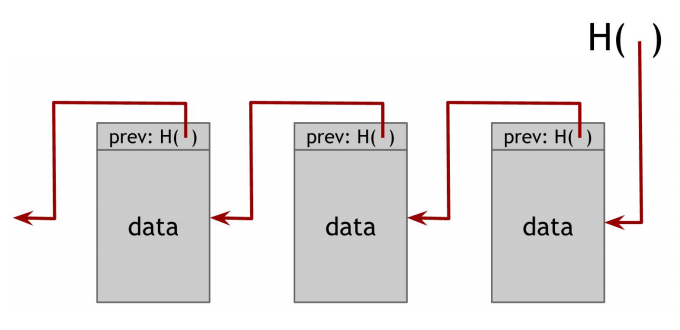
\includegraphics[width=0.9\textwidth]{go5}
  \caption{Fundamental Blockchain, Image Source: \cite{narayanan2016bitcoin}}
\end{figure}

\section{Problem Statement}

As alluded to above, one of the architectural components of Bitcoin is a modified linked list known as a \textit{blockchain}, demonstrated in Figure 1.2.
At a fundamental level a blockchain can be thought of as a linear collection of data elements, called nodes ($n_1, ..., n_n$). 
Each node, $n_1$, is pointed to by the subsequent node, $n_2$, by means of it's hash.
Therefore $n_2$ references a hash of $n_1$. 
One of the characteristics of this data representation format is that the integrity of the complete list can be easily verified with relatively low storage requirements, in fact by maintaining only the single hash at the head of the list.
This construct, introduced by Haber \& Stornetta \cite{haber1990time}, is integral to the Bitcoin specification and the implementation of a similar data model among members of a supply chain could provide some benefit. 
However as noted earlier the novelty of Bitcoin is not due to any one element but rather to the mutual co-dependence of many inter-related technical components.
In the chapters that follow we examine a subset of the these components and detail a methodology for utilizing them towards the creation of a more efficient and effective world-wide web, and perhaps a more efficient and effective world.

% \section{Outline \& Structure\label{sec:outline}}

% \\
% \\
% \textbf{Chapter \ref{cha:chapter2}}

% \\
% \\
% \textbf{Chapter \ref{cha:chapter3}}

% \\
% \\
% \textbf{Chapter \ref{cha:chapter4}}

% \\
% \\
% \textbf{Chapter \ref{cha:chapter5}}

% \\
% \\
% \textbf{Chapter \ref{cha:chapter6}}

% \\
% \\
% \textbf{Chapter \ref{cha:chapter7}}

% \\
% \\
% \textbf{Chapter \ref{cha:chapter8}} 





    \chapter{Framework for Symbiotic Development}\label{cha:chapter2}}

The concept of peer-to-peer applications is not new, nor is the concept of distributed hash tables. 
What emerged in 2008 with the publication of the Bitcoin white paper was an incentive structure that unified these two software paradigms with a set of economic stimuli to motivate the creation of a dedicated computing network orders of magnitude more powerful than the world's fastest supercomputers.
The purpose of which is the maintenance of a massive distributed database known as the Bitcoin blockchain.
Apart from the digital currency it enables, blockchain technology is a fascinating new computing paradigm with broad implications for the future development of the World Wide Web, and by extension, the further growth of Linked Data and the Semantic Web. This chapter is divided into two main sections, we first demonstrate how blockchain technologies can contribute towards the realization of a more robust Semantic Web, and subsequently we provide a framework wherein the Semantic Web is utilized to ameliorate blockchain technology itself.

\section{Background}

With the rise of the Bitcoin cryptocurrency the concept of distributed blockchain databases received wider attention.
Based on the distributed blockchain infrastructure a wide range of distributed applications can be built.
One unique approach in that regard is Etherum platform, which includes a Turing-complete programming framework aiming to realize so called ``\textit{smart contracts}''.
Similarly as blockchain technology can facilitate distributed currency, trust and contracts application, Linked Data facilitated distributed data management without central authorities.
In this article, we investigate how the blockchain and Linked Data concepts can be fruitfully combined to realize novel applications.
%Cryptographic hash tables in the form of Merkle trees, viz. blockchain, as popularized by the open-source Bitcoin project have been garnering significant attention in popular culture and media but to date have not been thoroughly examined in the context of the utility of its application to semantic technologies. 
%change this first sentence

One of the problems with the blockchain as a technology is the negative association it has inherited due to the illicit nature of some early applications of Bitcoin as a currency. Moreover the polarization of it's advocates, who often regard it as a panacea, i.e. ``\textit{the most important invention in the history of the world}''\footnote{\footnotesize{http://rogerver.com}}, and vehemence or apathy of its detractors, e.g. Jamie Dimon the chief executive officer of JPMorgan Chase, quick to write it off completely as a ``\textit{waste of time}''\footnote{\footnotesize{http://fortune.com/2015/11/04/jamie-dimon-virtual-currency-bitcoin}}, has contributed towards an environment wherein it is difficult to isolate the novel contributions of blockchain technology, of which there are some, and how they might be harnessed to improve the infrastructure of the Web, a development we regard as both desirable and actionable. 

This chapter proceeds with a two-pronged demonstration, first we provide an objective analysis of blockchain technology in the context of its relevance to the Semantic Web.
% In so doing we hit upon legacy issues in the design of the Web, and by implication the Linked Data infrastructure, that blockchain computing stands to resolve. 
With our framework firmly established we go on to describe a methodology for the implementation of several applications made possible through the integration of well known Semantic Web concepts within the computational architecture of the blockchain and set forth a benchmark for evaluating the validity of our approach.

In the subsequent sections we provide a high level description of the functional underpinnings of the Bitcoin blockchain and examine two technologies that extend the current blockchain in ways applicable to the contribution we describe above. 
Furthermore we demonstrate our model of a blockchain based URI naming scheme that positions the RDF data model in closer alignment with the concept of Cool URIs~\cite{timbernerslee1998}. 
Next is a description of the composition of an extensible ontology for blockchains and the resultant Linked Data ecosystem in the context of exploring the exchange of value within a network as well as the unification of the disparate technical nomenclature, towards creating a common understanding of analogous components existing in silos of the development landscape this open-source community continues to foster.
Finally we examine the case for novel semantic applications of decentralized Industry 4.0 platforms. 


\section{Context}

The blockchain facilitates a resilient and highly distributed ledger for recording transactions, attributing them to a specific node in a network, and ordering them in time. 
This is the functionality that undergirds the cryptocurrency Bitcoin (BTC), among others. This phenomenon is made possible through a process known as ``\textit{mining}'' whereby a large number of dedicated high-powered computers running application-specific integrated circuits (ASICs)~\cite{grantbrunner2013} process the transactions of the Bitcoin network in real time, competing with each other for a small fee associated with a new transfer in BTC in addition to a ``\textit{subsidy}'' in the form of a fixed amount of newly minted Bitcoins.
Data is permanently recorded in the Bitcoin network through files called blocks. 
A block is a record of some or all of the most recent Bitcoin transactions that have yet to be recorded in prior blocks. 
Mining is the process of adding transaction records to Bitcoin's public ledger of past transactions. 
This ledger of past transactions is called the blockchain as it is a chain of blocks. 
The blockchain serves to confirm transactions to the rest of the network as having been executed.

\subsubsection{Blockchain}

A useful analogy for conceptualizing blockchain technology is peer-to-peer (P2P) computing, wherein a distributed application architecture partitions work loads among equally privileged participants in an application, forming a peer-to-peer network of nodes.
A blockchain is a globally shared, transactional database, similar to the peer-to-peer file sharing system BitTorrent. 
All participants in a blockchain network can read the database. 
Where it diverges from P2P applications is in the ``\textit{consensus}'' mechanism. 
Changes in the database are performed by means of transactions, which have to be accepted by the participants in the network. 
Transactions are atomic (i.e. executed in full), durable (i.e. can not be altered) and cryptographically signed by the creator (guarding access to modifications of the database). 
\autoref{fig:block-chain-risk} illustrates the blockchain concept. 
Several transactions are bundled in a block and then executed and distributed among the nodes in the blockchain network. 
In case of conflicting transactions, the first one is given precedence and subsequent conflicting ones are discarded.

\begin{figure}[tb]
   \center 
   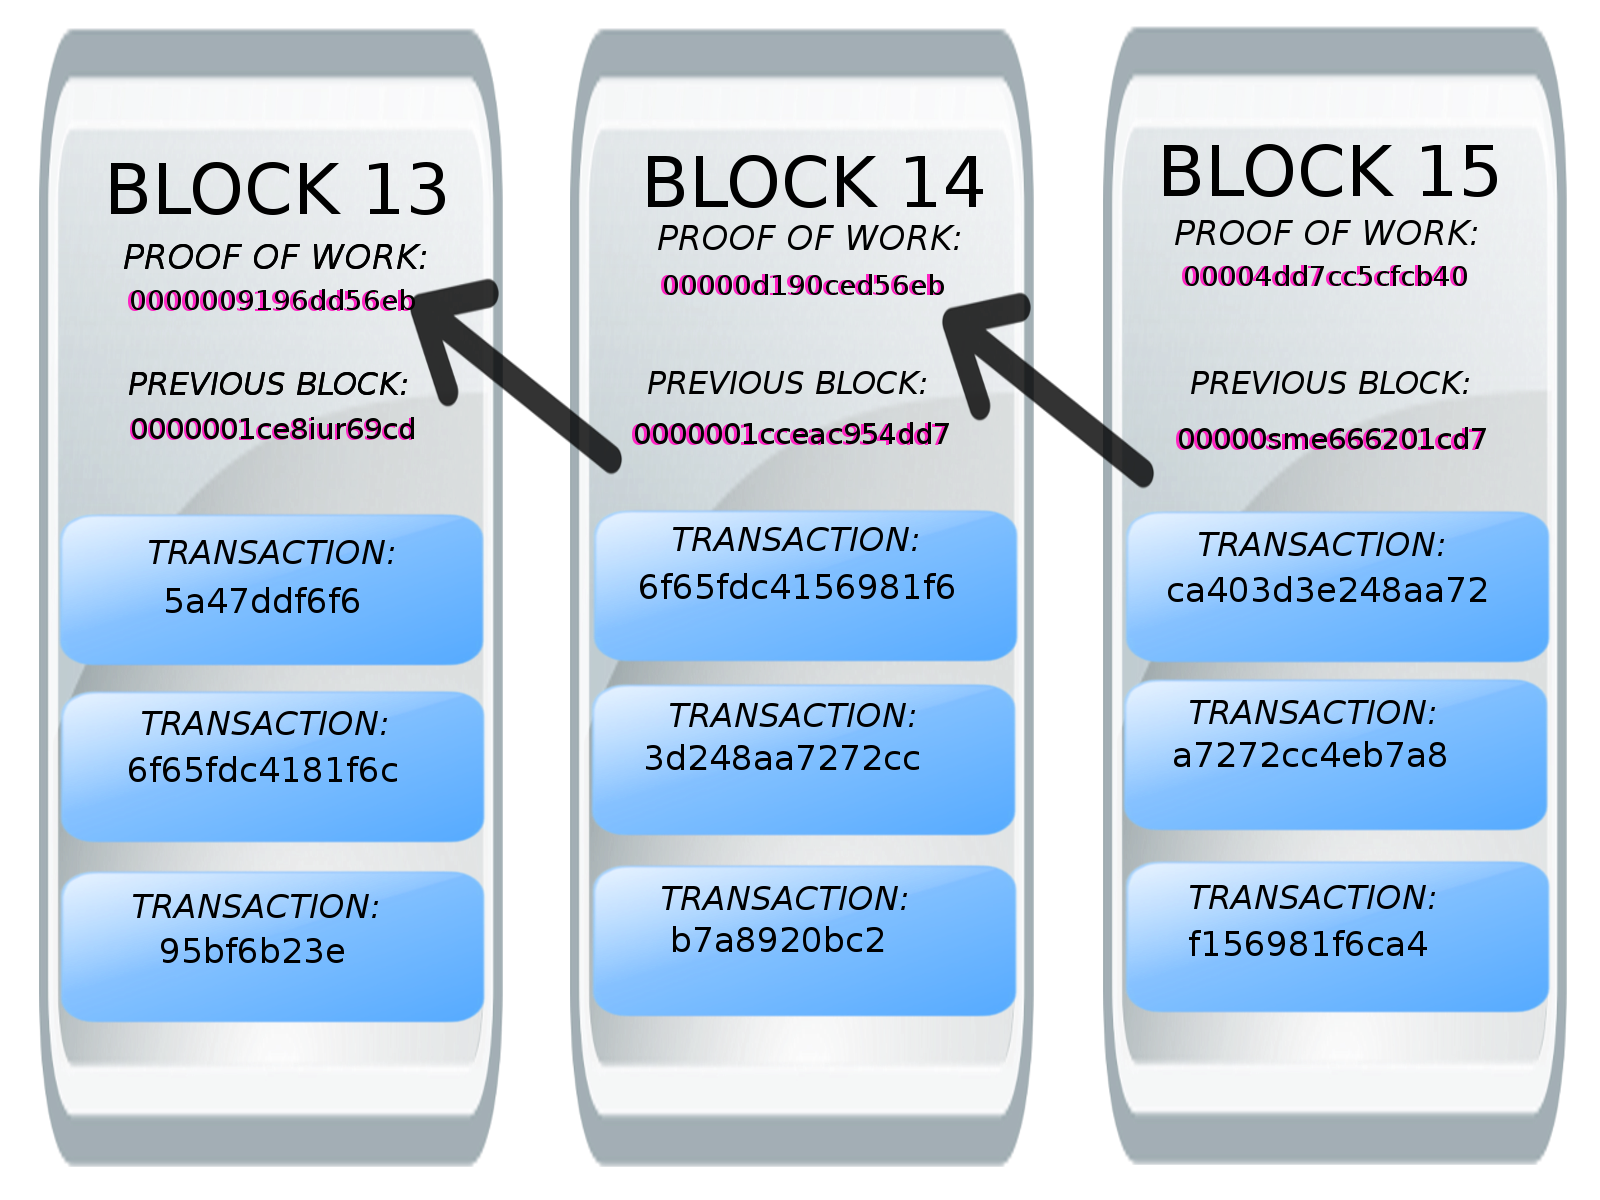
\includegraphics[width=.7\textwidth]{blockchain_sme}
   \caption{Illustration of a Blockchain} 
   \label{fig:block-chain-risk}
\end{figure} 
 

\subsubsection{Blockchain 2.0.}

The securing of a cryptocurrency network notwithstanding, there are a multitude of applications that can be run alongside, or in conjunction with the Bitcoin blockchain, taking advantage of the large amount of computational effort generated by the dedicated mining machines and the open access afforded to this processing power available to all holders of even nominal amounts, i.e. 0.00000001 (known as 1 \textit{Satoshi} after the author of the original white paper~\cite{whitepaper}), of BTC. 

Furthermore there are numerous forks of the original open-source Bitcoin code, known as ``\textit{altcoins}'', the majority of which implement negligible or generally uninteresting modifications. That said, in this paper we explore two of such forks that have extended the original blockchain concept in ways which can be utilized to provide useful and unique services, extending the blockchain concept in powerful ways. 

Bitcoin's scripting language allows one to store small amounts of metadata on the blockchain, which can be used to represent transactions more complex than simple exchange such as asset manipulation instructions, i.e. escrow services that cannot release a transaction without consent from multiple parties. 
These ancillary applications have come to be known collectively as ``\textit{Blockchain 2.0}''.

\subsubsection{``Smart Contracts''}

The original blockchain network can be regarded as a tool to execute a system of contracts focused on the application of value exchange. Altcoins such as Namecoin adapted this original ``\textit{currency application}'' of the technology into other applications, in the case of Namecoin, to DNS registration. 
Ethereum is another Altcoin project which attempts to build a more generalised blockchain technology; on which all transaction-based state machine concepts can be built, to provide to the end-developer a tightly integrated end-to-end system for building software on a hitherto unexplored compute paradigm in the mainstream: a trustful object messaging compute framework, i.e. performing non-trivial computations within the blockchain itself~\cite{wood2014ethereum}.
While the Bitcoin blockchain does allow very simple transactions (i.e. the transfer of funds from one account to another), Ethereum expands the concept of transactions to arbitrary complex contracts dubbed ``\textit{smart contracts}''. For this purpose, transactions contain an algorithmic description of the smart contract and Ethereum provides programming languages and APIs for devising the smart contract. 

\subsubsection{Ethereum Virtual Machine}

The Ethereum Virtual Machine (EVM) is the runtime environment for smart contracts in Ethereum.  It is sandboxed and completely isolated (i.e. code running inside the EVM has no access to network, filesystem or other processes). Smart contracts even have limited access to other smart contracts. 
In subsequent sections we explore how the extended functionality of ``\textit{smart contracts}'' could potentially facilitate a series of novel methods for the symbiotic development of blockchain technologies with the Semantic Web. 


\section{What can blockchain do for Semantic Web?}

In the preceding sections we examined the novel computational paradigm that blockchain as a technology makes feasible. In this section we will demonstrate ways in which blockchain technology can be applied in practice towards the actualization of a more resilient architecture for the Semantic Web. 

\subsection{Secure Resource Identifiers}

On the Semantic Web, all information is expressed in statements about resources.
Resources are identified by International or Uniform Resource Identifiers (IRI/URIs). 
While URIs are very beneficial, they also have some inherent weaknesses:

\begin{itemize}
    \item \emph{Centralization.} While individual URIs can be minted in a distributed fashion, the identifier generation relies on the centralized DNS system, which poses a single point of failure or attack.
    \item \emph{Persistence.} In case of intentional (e.g. a merger or acquisition of a legal entity) or unintentional (e.g. bankruptcy) events, the persistence of identifiers can not be guaranteed.
\end{itemize}

There are three key requirements which an ideal identifier system should fulfill:

\begin{enumerate}
    \item \emph{Secure:} dereferencing identifiers should not be prone to attacks, i.e. when retrieving the content of a website or resource the authenticity of the content should be ensured.
    \item \emph{Human-readable:} it should be possible to give identifiers intuitive names, which can be easily remembered by humans.
    \item \emph{Decentralized:} no central authority should control identifier creation and pose a single point of failure or attack.
\end{enumerate}

Zooko Wilcox-O'Hearn conjectured that no single kind of naming system can achieve more than two of these properties~\cite{wilcox2003names}.
Aaron Swartz~\cite{aaronswartz2011} described a naming system based on Bitcoin employing Bitcoin's distributed blockchain as a proof-of-work to establish consensus of domain name ownership.
These systems remain vulnerable to an attack wherein the reputation system is subverted by forging identities in the peer-to-peer network but is secure under Byzantine fault tolerance.

Namecoin implements the concept.
Namecoin is a decentralized open source information registration and transfer system based on the Bitcoin blockchain itself.
It enables users to dis-intermediate the Domain Name System (DNS) providers, one of the last bastions of centralization in the architecture of the modern web.

Practically speaking the issues identified above have afflicted the Semantic Web community in the past, e.g. the shuttering of Freebase by it's acquirer Google~\cite{2015}. 
Consider the semantic machine learning system NELL (Never-Ending Language Learning)~\cite{carlson2010toward}, which aims at remaining operational indefinitely. 
For such an ambition as this to be credible we must rely on a system that satisfies the aforementioned criteria, a system such as Namecoin. 
Consequently we have commenced the implementation of a fully functional mirror site to \texttt{dbpedia.org} under the top-level domain \texttt{dbpedia.bit}.
To achieve success in this endeavour there are some technical hurdles to overcome, we detail these now.  

On the protocol level, there are no constraints on URIs in Namecoin; names can be made up of arbitrary binary data with a length of 0 to 255 bytes. If we want a \texttt{.bit} DNS name, in Namecoin syntax the name should be structured as ``\texttt{d/example}'' where ``\texttt{example}'' must be a lower-case, valid domain name. 
New resources are assigned subdomains to \texttt{dbpedia.bit}. 
\autoref{fig:sparql} demonstrates a simple exemplary query on the de-referenceable blockchain based naming scheme for DBpedia under the domain `\texttt{dbpedia.bit}'.

\begin{lstlisting}[label=fig:sparql,caption=SPARQL query on \texttt{.bit} TLD,language=Javascript,basicstyle=\scriptsize \ttfamily,numbers=left,numberstyle=\tiny\color{mygray}]
PREFIX ex: <http://dbpedia.bit/exampleOntology#>
SELECT ?capital ?country WHERE {
  ?x ex:cityname      ?capital ;
     ex:isCapitalOf   ?y .
  ?y ex:countryname   ?country ;
     ex:isInContinent ex:Europe .
}
\end{lstlisting}


In terms of long-term viability, names on this system can be transferred and thus also sold. 
It is even possible to sell names in a trust-less way in exchange for Namecoin currency, since the transaction sending the name and the transaction paying the seller can be made atomic.
If a wallet owning a name disappears the name expires 36,000 blocks after the last update, so it will stay active for some time but then become available again for a new owner.

\subsection{Namecoin Access}

The Namecoin blockchain stores the pertinent information for navigating the \texttt{.bit} top level namespace. However, since \texttt{.bit} domain names, are not yet part of the standard domain name system, these can not be de-referenced without additional support. For example, there are \texttt{.bit} web proxy servers that will correctly handle these DNS requests in a browser as well as extensions for Firefox, Chrome and online look up services\footnote{\footnotesize{\texttt{http://namecha.in/name/d/domob}}}.
To dereference or retrieve resources from \texttt{dbpedia.bit} run the core client, using the ``\texttt{name\_show}'' RPC command,  e.g. ``\texttt{name\_show d/domob}'' on the debug console, or ``\texttt{namecoin-cli name\_show d/domob}'' on the shell.

\subsection{Storing data in the blockchain}

There are multiple ways to store data directly within the Bitcoin blockchain. 

\begin{enumerate}
 \item \emph{Value:} Encode data in the number of \textit{Satoshis} being sent to an address.
 \item \emph{Vanity address:} Brute force through keys until arriving at an address that encodes personalized data, i.e. encoding the pattern \texttt{1ESWC} as in \\ \texttt{1ESWCs3d48d3198863e75m7f9d1827cdfc6048e}.
 \item \emph{MultisigAddress:} These are more complex Bitcoin addresses that require more than one signature from a private/public key to redeem the value.
 \item \emph{OP\_RETURN:} Command in the Bitcoin scripting language that was specifically added to permit the inclusion of metadata (up to 40 bytes) on the blockchain.
\end{enumerate}

Moreover, units of real world value distinct from the blockchain can be affixed to nominal amounts of BTC, as stock certificates were once printed on paper, the paper itself has some small value, but it represents (presumably) a greater value insofar as it is the physical manifestation of part ownership in some corporation. A so-called ``\textit{colored coin}'' is used in conjunction with a wallet specially tailored to recognize such additional information, thereby conferring the benefits of the blockchain's distributed trust mechanism to a multiplicity of novel applications~\cite{timswanson2014}. We regard this as the most feasible medium of synthesis between blockchain and representations of information in the Linked Data ecosystem.  

\section{What can Semantic Web do for blockchain?}

Through formal semantic knowledge representations we have created an ontology for capturing data within the blockchain.
The utility of such a shared conceptualization is twofold.
Primarily it facilitates a shared understanding of blockchain concepts between humans.
Additionally, by exposing the blockchain data according to an ontology, we enable interlinking with other Linked Data to conduct formal reasoning and inference. 

Our work extends, in keeping with the principles of ontology reuse~\cite{grangel2015Convention}, an initial vocabulary created by Melvin Carvalho~\cite{melvincarvalho2013}\footnote{\url{http://cc.rww.io/vocab}}. In so doing we formalize key concepts such as wallets, blocks and transactions.
We render the vocabulary suitable for graphical analysis using Visual Notation for OWL Ontologies~\cite{VOWL2}.
%cite irlan

\begin{figure}[tb]
   \center 
   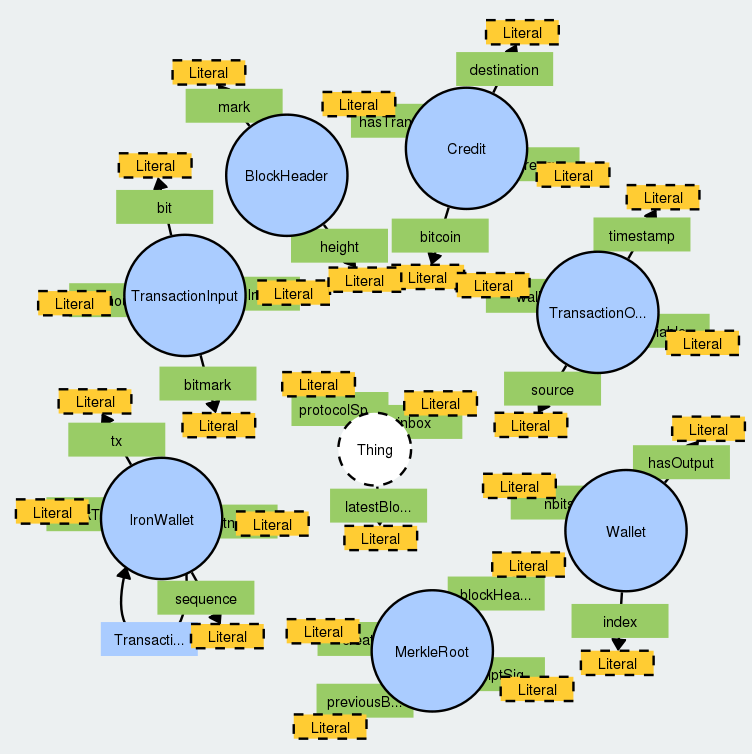
\includegraphics[width=.5\textwidth]{vocab_visualization_0}
   \caption{Diagram Illustrating the Ontology} 
   \label{fig:viz}
\end{figure} 


\subsection{Exploring the blockchain}

One of the beneficent features of blockchain technology is that it increases transparency through a completely open ledger (in order to establish trust) while simultaneously ensuring anonymity through preserving accounts behind their public keys.
However, the transparency is currently only established on a technical level.
For humans it is cumbersome to track transactions and accounts on the blockchain.
The vocabulary based representation of the blockchain data increases transparency and analysis capabilities for human users.
We propose a model whereby transactions are represented in RDF, and thereby support the linking of wallets related by transactions to follow exchange activity around the network.
The first generation of blockchain explorers\footnote{\url{http://blockchain.info/}} are limited in efficacy by the aforementioned issue, as in \autoref{fig:api} transactions represented in JSON are notoriously difficult to follow throughout the network.

\begin{lstlisting}[label=fig:api,caption=JSON Exploration API Output,language=Javascript,basicstyle=\scriptsize \ttfamily,numbers=left,numberstyle=\tiny\color{mygray}]
{
    "balance" : 43.50100000,
    "errors" : "",
    "paytxfee" : 0.005,
    "proxy" : "",
    "connected" : 0,
    "testnet" : false,
    "difficulty" : 1733207.51384839,
    "blocks" : 179602
}
\end{lstlisting}

Our working ontology, implemented in OWL, melds the Carvalho vocabulary with the Bitcoin API calls list \footnote{\url{http://en.bitcoin.it/wiki/Original_Bitcoin_client/API_calls_list}}.
Furthermore we include functionality to actualize the working model of Ethereum smart contracts. 
However, since Ethereum is in an early stage of development, further changes are likely to be required in the future.
Additions comprise in particular the ability to bind the validity of transactions to certain geospatial locations, to facilitate the generation of so-called ``\textit{smart property}'', property whose ownership is controlled via the blockchain, with access contingent upon ownership of a public/private key pair~\cite{szabo1997idea}.


\subsection{Testnet Block Explorer}

The term ``\textit{testnet}'' is used to refer to a blockchain created by forking the original Bitcoin code repository\footnote{\footnotesize{\texttt{http://github.com/bitcoin}}}, configuring several nodes, and commencing the mining process on one's own machine or local network. 
This practice is the primary mechanism for blockchain-based experimentation. 
Naturally testnet coins are distinct from Bitcoins ``\textit{in the wild}'', they are not intended to denote monetary value, permitting iterative development without large capital outlays or adverse effects to the main Bitcoin blockchain.

Transactions can be described using our working blockchain vocabulary\footnote{\footnotesize{\texttt{http://github.com/smenglish/block.chain.ontology}}}. 
The supplementary information thereby created can be injected into the blockchain by one of several methods: 

\begin{itemize}
    \item The coinbase field of a mined block allows for hexadecimal data which can hold 560 bytes.
    
    \item Use of a ``\textit{colored coin}'' and corresponding specialized wallet.
    
    \item Multiple outputs can be used for a transaction such that each holds hexadecimal data. This would imply dust value outputs (outputs of $\leqslant{}$ 0.00005640 BTC) and in practice would contribute relatively ``\textit{large}'' amounts of superfluous data to the blockchain, a technique known as ``\textit{bloating}'' and generally considered bad practice.
    
    \item Hexadecimal data from a multi-signature transaction can also be used to encode information.
\end{itemize}

The open-source \textit{Block Explorer}\footnote{\footnotesize{\url{http://testnet.blockexplorer.com}}} can be used to examine the contents of transaction blocks, i.e. recipient and sender addresses or code snippets delivered through counterparty exchanges and recorded in the testnet blockchain as depicted in \autoref{fig:testnet}.  


\begin{lstlisting}[label=fig:testnet,caption=Testnet Output Specifying Counterparties,language=Javascript,basicstyle=\scriptsize \ttfamily,numbers=left,numberstyle=\tiny\color{mygray}]
{
  "sender": "1QBb5MpKUMiqc27wrD2QDRsC9gZYyy49",
  "recipient": "1AdCDBz2VmhUZDyDbibMo2QGGSjt93zbF",
  "size": 479,
  "merkleroot": "f5b3309272c5fcb3febb0f09986e77158",
  "time": 1440604813,
  "bits": "1814434",
  "difficulty": 54256630327.88996,
  "reward": 25,
}
\end{lstlisting}


\begin{figure}[tb]
   \center 
   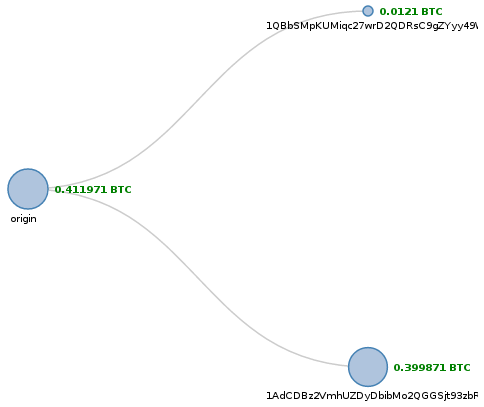
\includegraphics[scale=0.3]{Alfa_beta_tree}
   \caption{Graphical Representation of Linked Transaction Counterparties} 
   \label{fig:block-chain-explorer}
\end{figure} 


Describing transactions in the context of Linked Data, as contrasted with a less expressive representation, facilitates a number of benefits. Binding transactions to individuals or organizations in furtherance of transparency, or to a particular geographic location as in the execution of so called ``\textit{smart property}'' arrangements. 
In \autoref{fig:block-chain-explorer} we demonstrate how such a transaction propagates through our network, with many of such applications taking place there is an emergent linked data ecosystem of value transmission.

\subsection{Standardization}

At the time of writing, contributors to the core Bitcoin blockchain code number less than four hundred individuals\footnote{\footnotesize{\texttt{http://github.com/bitcoin/bitcoin/graphs/contributors}}}.
If blockchain technology will become an integral component in the infrastructure of the modern Web it will necessitate its being thoroughly understood by a much greater community of developers. 
The lack of such a common understanding was cited as one of the premiere issues impeding this continued growth of blockchain technology by Gavin Andreeson the successor to Satoshi Nakamoto as the principal maintainer of the bitcoin code base~\cite{jonmatonis2012}.
Accordingly we have contributed to a the creation of the first publicly-available\footnote{\footnotesize{\texttt{http://github.com/smenglish/block.chain.ontology}}} shared ontology to facilitate improved comprehension within this burgeoning development community.

\subsubsection{Industry 4.0}

The fourth industrial revolution, Industry 4.0, is a collective term embracing a number of contemporary automation, data exchange and manufacturing technologies. It had been defined as ``a collective term for technologies and concepts of value chain organization''~\cite{nirjargandhi2015} which draws together Cyber-Physical Systems, the Internet of Things and the Internet of Services, and critically Semantic Technologies. In this section we consider the ways the union of blockchain technologies and the Semantic Web is shaping the continued development of this latest phase of industrialization. 

\begin{figure}[tb]
   \center 
   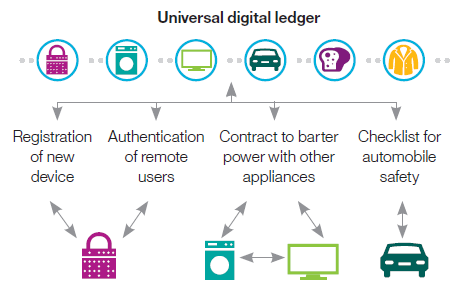
\includegraphics[width=.7\textwidth]{i40ledger}
   \caption{Using the blockchain as universal digital ledger for Industry 4.0 transactions~\cite{DeviceDemocracy}.} 
   \label{fig:passport}
\end{figure} 

Using blockchain technology, a fully decentralized data marketplace for sensor data could be realized. Instead of establishing individual contracts with every data provider, the blockchain could become a clearing house for sensor data exchange. In \cite{DeviceDemocracy} IBM describes the vision of employing the blockchain as universal digital  ledger for Industry 4.0  transactions, such as registration of devices, authentication of users, bartering and supply chain transparency. For these applications, a comprehensive semantic description of the products and half-products exchanges in the value chain is essential. Finally, such descriptions should be linked with related information contained in other systems of the participating companies.

As a concrete example, \autoref{fig:provenance} shows the core logic of a Ethereum ``\textit{smart contract}'', which represents an address on an Industry 4.0~\cite{christopherbrewster2014} supply chain management platform.
The \texttt{mortal} super-class defines the initialization and finalization of the smart contract.
The contract \texttt{accountManager} itself comprises a potentially large array indexed by accounts with each entry comprising two pieces of information, an URI identifying a certain product type and possibly linking to further information about the product as well as a hash identifying a concrete product realization or production batch.
The public key authentication of Ethereum ensures only a certified account owner can update information about the provenance of his products or semi-products.
If other participants in the supply chain, refer to such a product or semi-product (e.g. in a way that it is incorporated/used within their product) the public ledger based on the Etherum blockchain ensures, the provenance of products and their incorporated half-products and ingredients can be traced back along the supply chain.

\begin{lstlisting}[label=fig:provenance,caption=Simple Ethereum Contract on Industry 4.0 Platform \texttt{Provenance.org}~\cite{juttasteinerjessibakergavinwood2013},language=Javascript,basicstyle=\scriptsize \ttfamily,numbers=left,numberstyle=\tiny\color{mygray}]
contract mortal {
    /* Define variable owner of the type address*/
    address owner;
    /* this function is executed at initialization and sets the owner of the contract */
    function mortal() owner = msg.sender;
    /* Function to recover the funds on the contract */
    function kill() if (msg.sender == owner) suicide(owner);
}
contract accountManager is mortal {
    /* data structure to hold accounts*/
    struct Account {
        string uri;
        bytes32 hash;
    }
    /* mapping of accounts to data*/
    mapping (address => Account) accounts;
    function setAccount(string uri, bytes32 hash) returns (bool)
        return setAccount(msg.sender, uri, hash);
    function setAccount(address account, string uri, bytes32 hash) returns (bool) {
        bool rv = msg.sender == owner || msg.sender == account;
        if (rv) accounts[account] = Account(uri, hash);
        return rv;
    }
    function readAccountUri(address account) constant returns (string)
        return accounts[account].uri;
    function readAccountHash(address account) constant returns (bytes32)
        return accounts[account].hash;
}
\end{lstlisting}


\section{Discussion}

In this chapter we have endeavoured to catalogue the results of a thorough analysis of blockchain technology in terms of it's applicability as a computational paradigm to the Semantic Web and Linked Data community. Furthermore we have presented the results of our initial efforts to fuse these two constructs in mutually beneficial ways by extending the traditional Linked Data naming convention, providing an ontology for representation of elements and events in the blockchain ecosystem, and building a procedure for Link Data representation of transactions in a blockchain network. We have done a first step towards synergisticly integrating two promising decentralized data management technologies, Linked Data and blockchains.
It is the first step on a larger research agenda aiming to realize a truly distributed, democratic and domain-agnostic knowledge system.

% At present we are undertaking efforts to apply our approach more generally to the Bitcoin blockchain itself, we are interested in a comprehensive graphic analysis in RDF of the entire Bitcoin blockchain, specifically one that is generalizable to \textit{altcoins} as well. The dynamic nature of the Ethereum implementation codebase made it difficult to implement and test some of the ideas described in this article. We plan to create a comprehensive implementation and evaluation of integrating the Linked Data concepts into the Ethereum blockchain.
    \chapter{Credential Certification Mechanism\label{cha:chapter3}}

\begin{displayquote}
``\textit{What is all knowledge except recorded experience}'' \\- Thomas Carlyle (1795 - 1881)
\end{displayquote}
% observed philosopher 

The Semantic Web has been described as heralding the age of ``Web 3.0''. 
Increasingly this accolade is applied to blockchain technologies.
This chapter focuses on the problem of recognizing achievement in the emerging realm of massive open online courses (MOOCs) in addition to other non-traditional educational environments, to demonstrate the practical applicability of our approach. 
We evaluate the technical work we have undertaken towards realization of the benchmarks described in the previous section with the introduction of a blockchain-based decentralized application for the certification of academic credentials. 
Although blockchain is a relatively recent phenomena it draws on a rich history of pioneering research. Recognizing the achievements of our peers, and the industrial efforts in the domain, we consider the related work and juxtapose it with our own implementation.

% \autoref{fig:passport} depicts a scenario of how a smart contract platform such as Ethereum could support micro and standard accreditation within a higher educational setting. Educational establishments including universities and MOOC companies such as FutureLearn develop and deploy courses and award recognition of student achievement through certificates, micro-certificates and badges. 
% Students take courses and gain recognition after registering for and completing courses through certification. 
% In an era of re-skilling and lifelong learning\footnote{\footnotesize{No 21 year old on completion of a bachelor's degree will have gained all the skills he or she requires for the rest of his/her life}} students will increasingly take a variety of courses from a variety of providers over a longer period of time. There is a need in this context for students to be able to collect and store all their informal and formal qualifications in a fashion that makes these easily accessible to relevant parties such as potential employers and educational organisations. 
% The above process can be supported by two decentralized blockchain based applications (\DJ{}Apps) running on the Ethereum network. A Certificate Issuing and Validation \DJ{}App would handle the publication of signed certificates within a blockchain. Secure signatures would tie all certificates to the specific issuing educational institution and the receiving student. Because of the nature of blockchains the certificates would remain valid even if the issuing organisation ceased to exist. Recently, the University of Nicosia has placed all the certificates for its free introductory MOOC ``\textit{An Introduction to Digital Currencies}'' within the Bitcoin blockchain.\footnote{\footnotesize{\texttt{http://digitalcurrency.unic.ac.cy/certificates}}}

\begin{figure}[tb]
  \center 
  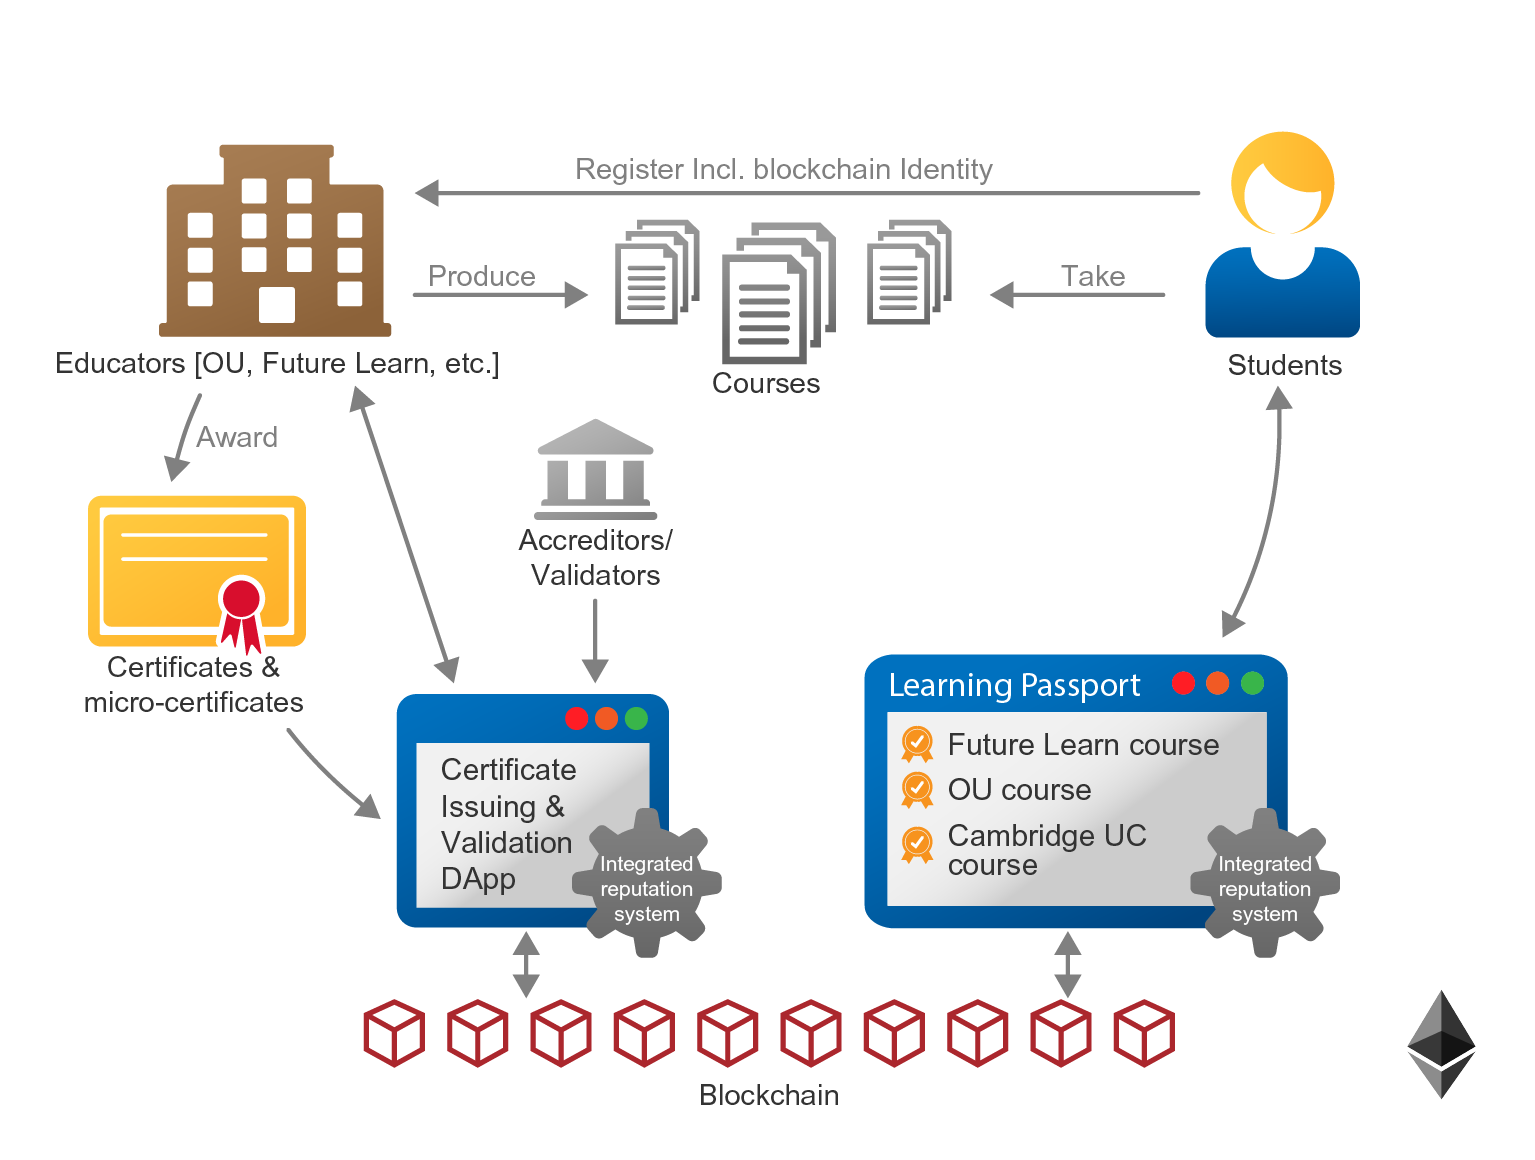
\includegraphics[width=.7\textwidth]{passport}
  \caption{A scenario of how blockchains and smart contracts can support accreditation and certification in higher education} 
  \label{fig:passport}
\end{figure} 

% A Learning Passport \DJ{}App would enable learners to easily view and manage all recognition of their learning no matter if informal or formal. These might include badges collected for course completion from MOOCs and formal degree course certificates. 
% Each of these two \DJ{}Apps would incorporate evaluation and reputation services. Certificates can be verified partly through reputation, but also be stored as credentials on the platform. For example, a verified credential proving certain prerequisites at one institution can allow a student to easily enroll in a higher level course at another. This allows the platform to operate with little overhead. Evaluation and reputation services would allow teachers and students to match their learning styles effectively. It will also set the stage for self-regulation of the system. Semantics can help in supporting interoperability issues in the above scenario. Namely:
% \begin{itemize}
%     \item Mapping from university and educational establishment data structures into the data structures as required by blockchain transactions and for the smart contracts.
%     \item Semantically, indexing template smart contracts and transactions for re-use.
%     \item Mapping between the Learning Passport data format into arbitrary certification and badging systems.
% \end{itemize}

\subsection{Credential Certification via Ethereum Virtual Machine}

Central mediation of services has become a bulwark of the Web. 
Common functions that are typically in the domain of central authorities include escrow/dispute resolution (e.g. eBay, AirBnB), identity management (e.g. Google+, Facebook). 
The \emph{Ethereum project} as created a blockchain with a built-in programming language. 
It is a platform that creates a virtual machine designed to be run by all participants in the peer-to-peer ``mining'' network. 
The purpose of which is to allow people to write decentralized applications (stylized as \textit{\DJ{}apps}) using blockchain technology. 
Although the project is relatively new \cite{wood2014ethereum} it holds the promise of affording users the ability to read and write to a blockchain both (quasi-Turing complete) executable code as well as data. 
The Enigma project from MIT is a related effort \cite{zyskind2015enigma}.

Traditional applications and web portals act mainly as a unified front-end to aggregate clients and provide the services of a particular entity. 
As conceptualized by the Ethereum project a \DJ{}app is a tool for people and organizations to act as counter-parties to an exchange without any such centralized intermediary.
A \DJ{}app is an application which serves some function for its users, but which has the salient characteristic that the application does not depend on the ongoing existence of any one actor. 
Some examples of proto-\DJ{}apps include BitTorrent for file sharing and of course Bitcoin for currency. 
The goal of the Ethereum project is to allow developers to generalize peer-to-peer network and blockchain technologies for a myriad of purposes.

The \emph{Ethereum Virtual Machine} (EVM) is the runtime environment for \DJ{}apps.  It is completely isolated (sandboxed) such that code running inside the EVM has no access to network, other processes, or the local filesystem.
Essentially the EVM is aiming to become a blockchain (viz. large decentralized computing network) with a multiplicity of nodes that collectively have the ability to maintain an internal database, execute code and communicate among one another.
In subsequent sections we explore how \DJ{}apps can facilitate a series of novel methods for the symbiotic development of blockchain technologies and the Semantic Web as applied to contemporary education methodologies. 

One of the defining characteristics of the $21^{st}$ century has been the proliferation of highly novel mediums by which people all over the world are empowered to share and consume information. 
This paradigm has given rise to new industries and is having a profound impact on well established ones. 
In this environment new opportunities are created for individuals with the appropriate proficiencies and accordingly the process of skill acquisition is one of the strongest indicators of societal change.

\subsection{Recognition of Credentials}

\emph{Massive Open Online Courses} (MOOCs) typically comprise a lecture series including accompanying material, focused on a particular subject, created for broad distribution across the Internet with largely unrestricted access for interested participants. 
Since their inception MOOCs have consistently attracted staggering numbers of students, typically in the hundreds of thousands.  
What is the reason for this popularity?

The increasing sophistication of statistical models that drive automation processes and machine learning are having a substantive impact on the economic landscape and are projected to make large numbers of jobs redundant in the coming years. 
This situation is merely one example in a cadre of changes that reflect a larger trend which might be described as something approaching a tectonic shift in the fundamental factors that drive the global economy. 
The rapid growth and demise of platforms and frameworks, the tools that support the dynamic response of industry to the increasingly mercurial needs of consumers, fuels a demand for educational resources that can keep abreast of the core competencies needed to distinguish oneself in the highly competitive job market.

\subsection{Impetus to Success}

The New York Times labeled 2012 ``the year of the MOOC'' \cite{laurapappano2012} with the emergence of a number of successful online education platforms backed by large industry actors and top universities.
In the intervening years there has been a diminution in the amount of media attention surrounding MOOCs, due (in no small part) to the low numbers of students that remain involved with the course through to successful completion. 
It has been strongly conjectured that one of the primary causes behind these disappointing statistics is the fact that there is considerable uncertainty as to how exactly the achievements benchmarked in MOOCs should be recognized. 
We focus particularly on MOOCs as an application scenario for using blockchain technology to certify learning achievements.
Learning today takes place in a context of new interactions between formal and informal learning. 
This is characterized by the changing role of teachers, the impact of social media and the students active participation in the design of learning activities.
Expertise in a domain might be gained through participation in a Meetup event, continued involvement in a question answering platform, thoughtful contemplation of recorded video content, or through a multiplicity of channels. 
All of these non-traditional educational mediums are marginalized by our current system of honouring credentials.

\subsection{Learning passport}

\autoref{fig:passport} shows a scenario of how a smart contract platform such as Ethereum could support micro and standard accreditation within a higher educational setting.
Educational establishments including universities and MOOC providers such as \emph{FutureLearn}\footnote{\url{http://www.futurelearn.com/}} develop and deploy courses and award recognition of student achievement through certificates, micro-certificates and badges. 

Students take courses and gain recognition after registering for and completing courses through certification. 
In an era of re-skilling and lifelong learning\footnote{No 21 year old on completion of a bachelor's degree will have gained all the skills he or she requires for the rest of his/her life} students will increasingly take a variety of courses from a variety of providers over a longer period of time. 
There is a need in this context for students to be able to collect and store all their informal and formal qualifications in a fashion that makes these easily accessible to relevant parties such as potential employers and educational organisations. 
The above process can be supported by two decentralized blockchain based applications (\DJ{}Apps) running on the Ethereum network. 
A \emph{Certificate Issuing and Validation} \DJ{}App would handle the publication of signed certificates within a blockchain. 
Secure signatures would tie all certificates to the specific issuing educational institution and the receiving student. 
Because of the nature of blockchains the certificates would remain valid even if the issuing organisation ceased to exist. 
Recently, the University of Nicosia has placed all the certificates for its free introductory MOOC ``\textit{An Introduction to Digital Currencies}'' within the Bitcoin blockchain\footnote{\url{http://digitalcurrency.unic.ac.cy/certificates}}.

A \emph{Learning Passport} \DJ{}App would enable learners to easily view and manage all recognition of their learning no matter if informal or formal. 
These might include badges collected for course completion from MOOCs and formal degree course certificates. 
Each of these two \DJ{}Apps would incorporate evaluation and reputation services. 
Certificates can be verified partly through reputation, but also be stored as credentials on the platform. 
For example, a verified credential proving certain prerequisites at one institution can allow a student to easily enroll in a higher level course at another. 
This allows the platform to operate with little overhead. 
Evaluation and reputation services would allow teachers and students to match their learning styles effectively. 
It will also set the stage for self-regulation of the system. 
Semantics can help in supporting interoperability issues in the above scenario, namely:
\begin{itemize}
    \item Mapping from university and educational establishment data structures into the data structures as required by blockchain transactions and for the smart contracts.
    \item Semantically, indexing template smart contracts and transactions for re-use.
    \item Mapping between the Learning Passport data format into arbitrary certification and badging systems.
\end{itemize}

\section{Decentralized Application (\DJ{}App) for Education}

As stated above Ethereum is a platform intended to facilitate the development of decentralized applications (\DJ{}apps) using blockchain technology. 
A foundational ingredient in the efficient operation of programs on this distributed application platform is ``Ether''. 
This is a form of payment made by the users of the network to the machines executing their code. 
Ether is the incentive ensuring that developers write applications that do not waste resources, e.g. running endless loops on the platform, it also ensures that users are compensated for the contribution of their computation time and/or memory space.

Recent work at The Knowledge Media Institute (KMi), research and development arm of The Open University, has been centered around the implementation of a decentralized application, which enables crowd-based recognition of educational activity on the \emph{FutureLearn} and \emph{OpenLearn}\footnote{\url{http://www.open.edu/openlearn/}} platforms. 

\begin{figure}[!ht]
  \centering
      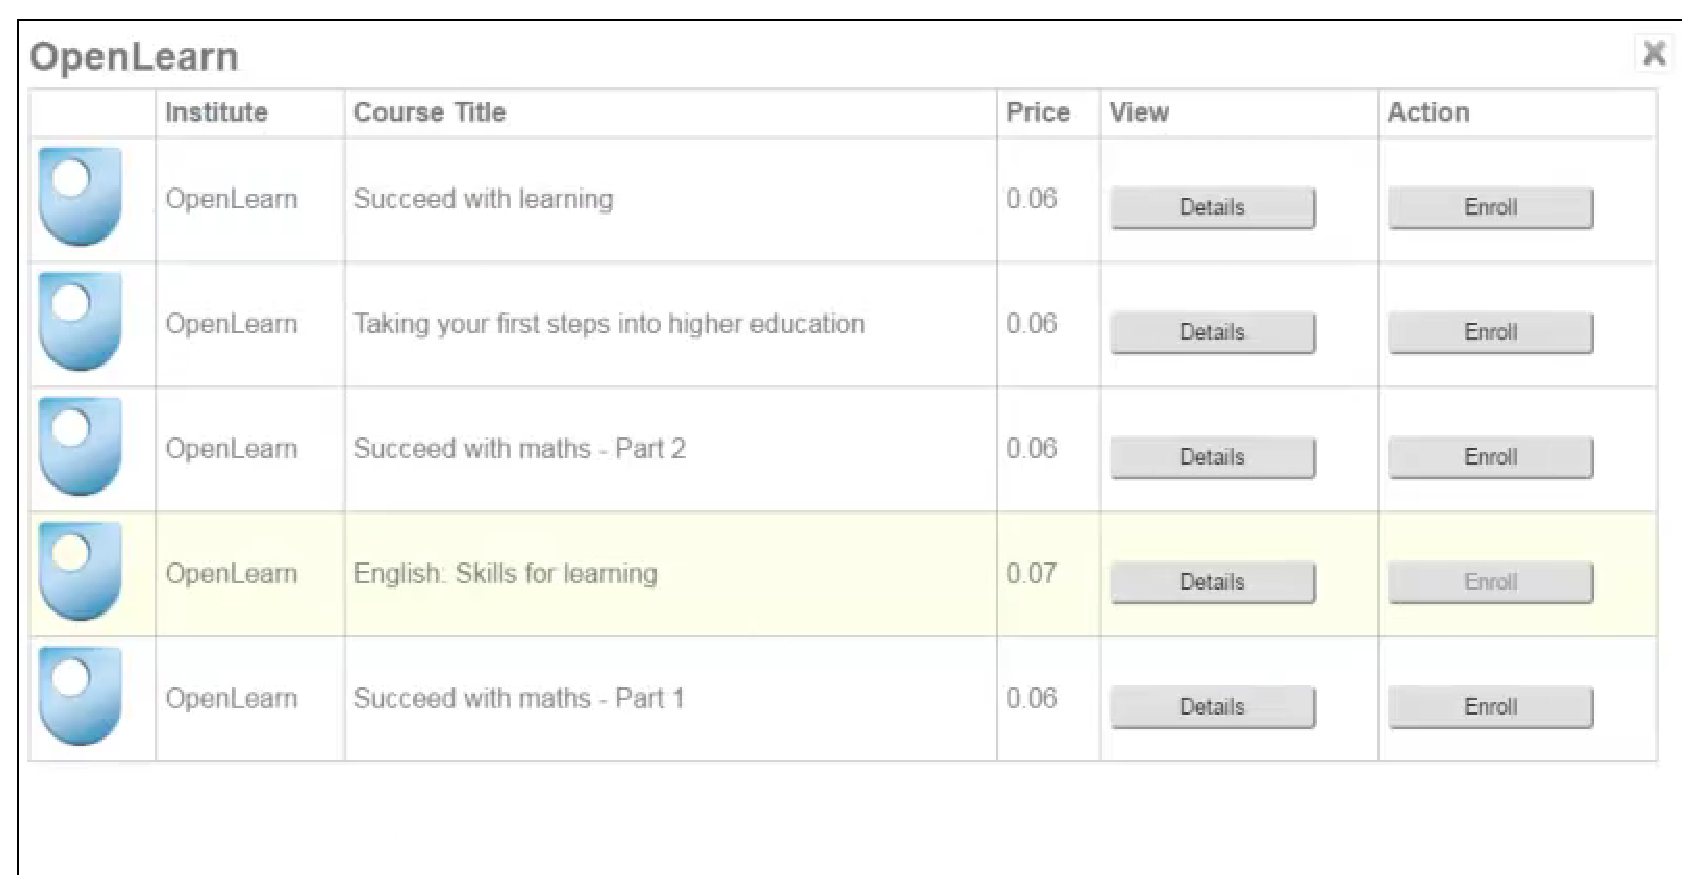
\includegraphics[width=0.69\columnwidth]{plat}
  \caption{Platform view.}
    \label{fig:xyz}
\end{figure}

The \DJ{}apps provides students the ability to enroll in courses using Ether funds, receive certifications of achievement, called ``awards'' and aggregate the awards in a sharable common interface. 
In this ecosystem the users, viz. students and administrators, manage enrollment, and remuneration (using Ether), in addition to the assignment of credentials all on the blockchain.   
On the Ethereum network a \DJ{}app consists of two parts: a frontend, written in HTML, and a backend, essentially the database of the application. 
We have developed a fully functional prototype of such a system, demonstrated in \autoref{fig:xyz}. 

\begin{figure}[!ht]
  \centering
      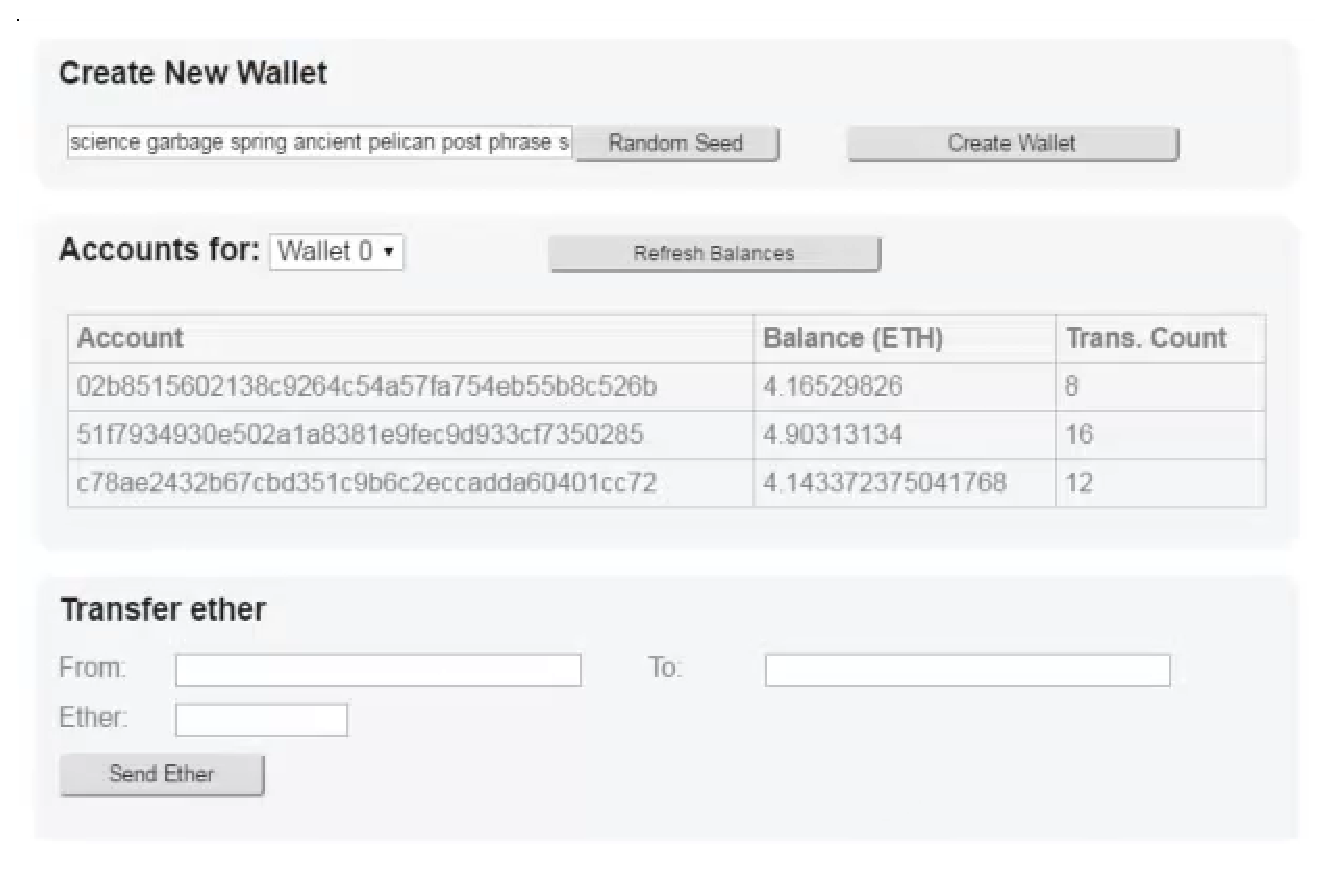
\includegraphics[width=0.69\columnwidth]{wallet000}
  \caption{Prototype of ``\textit{Student Browser}'' frontend.}
\end{figure}

From the main element ``My Wallets'' view students manage their Ether (available funds) account. 
Users create one or more wallets, and use them to transfer funds between different actors, e.g. a transmission of their Ether to an online learning platform such as \emph{FutureLearn}. 
There is a profile area wherein users can establish their identity by associating it with a known public key.
Accordingly an individual wallet account is bound to a name and an icon. 
Subsequently this account can be indicated as the ``current account'' and used to enroll in a course. 

\begin{figure}[!ht]
  \centering
      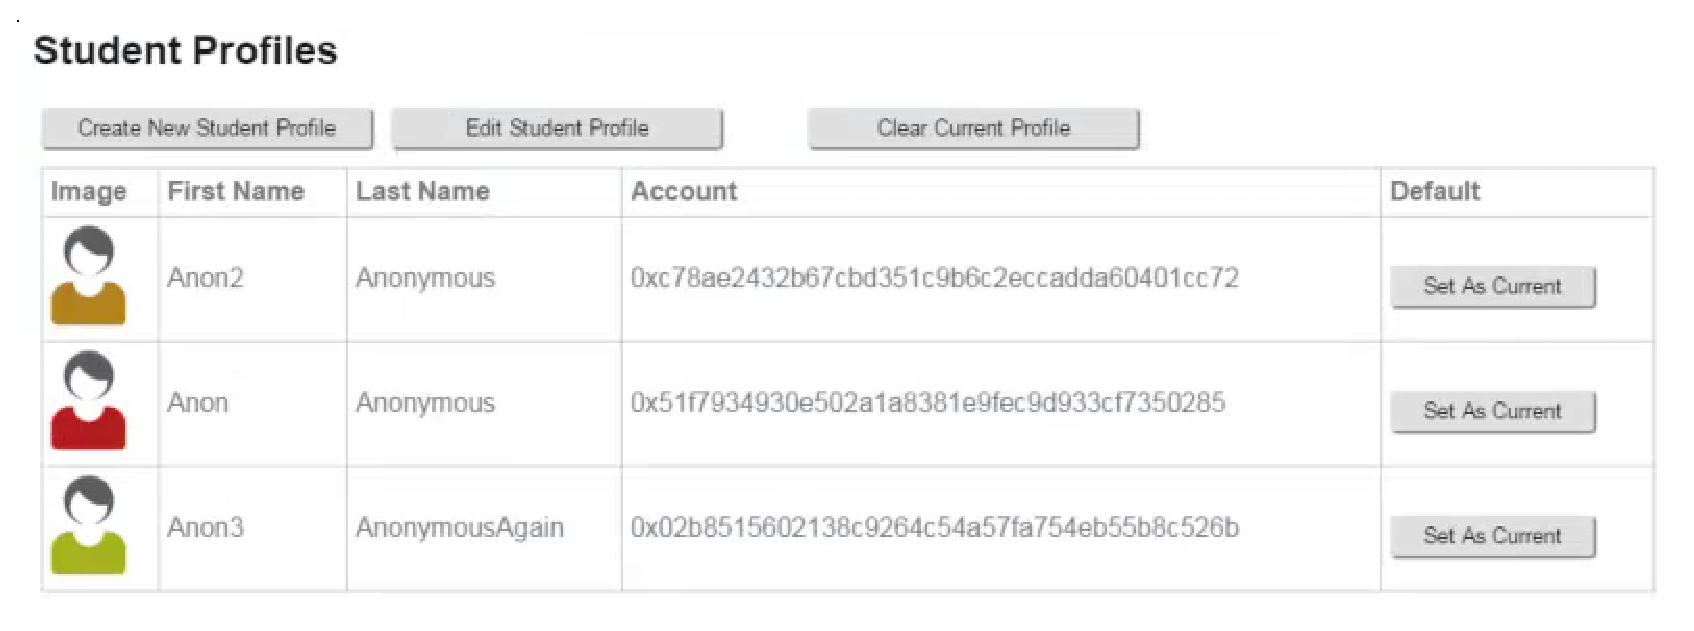
\includegraphics[width=0.69\columnwidth]{stupo}
  \caption{Dashboard view of multiple different user accounts.}
\end{figure}

The embedded \DJ{}app Store contains course selections from multiple sources, among them both \emph{FutureLearn} and \emph{OpenLearn} and are anticipating content from \emph{Fraunhofer Academy}\footnote{\url{http://www.academy.fraunhofer.de/en.html}} and \emph{SlideWiki}.

To register for a course in the system a user must initiate the process with a click-through of the ``Register'' button, this will prompt a pop-up box with a password input screen, since subsequently a monetary transaction (using Ether) will take place. 

\begin{figure}[!ht]
  \centering
      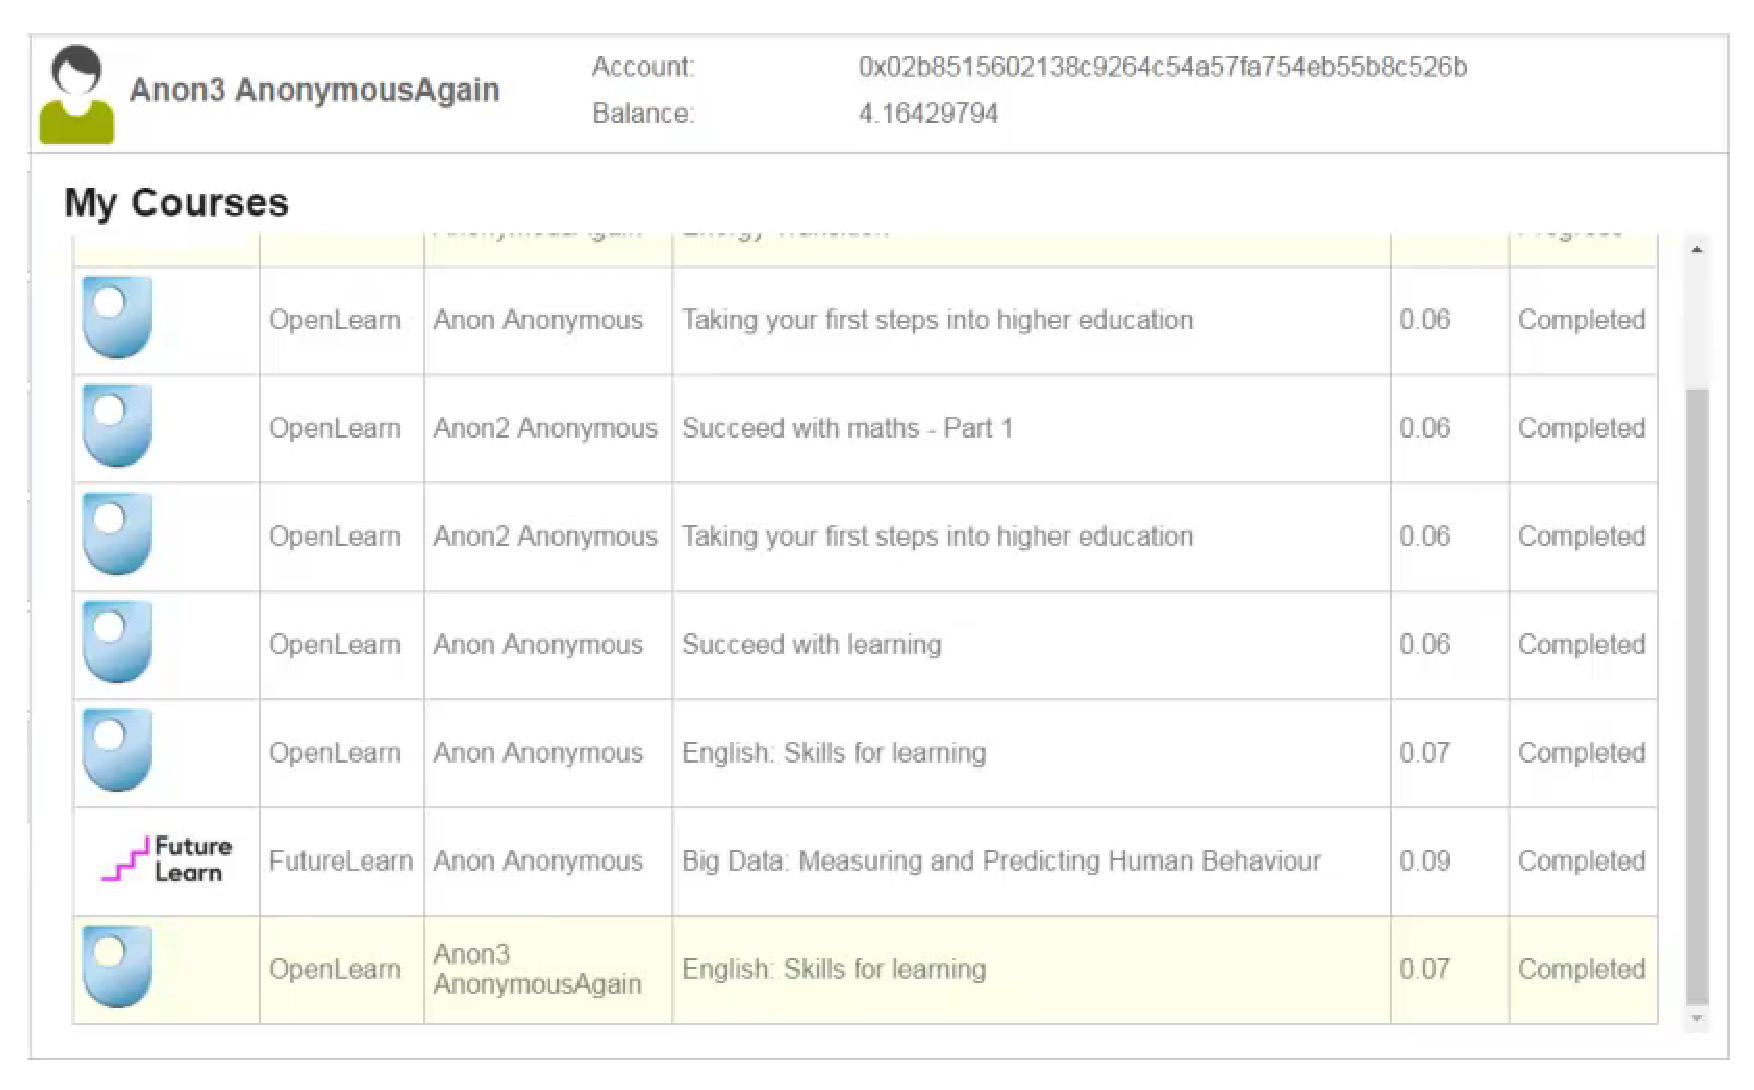
\includegraphics[width=0.69\columnwidth]{kor}
  \caption{Course Dashboard.}
\end{figure}

Concurrently with this interchange we can see a transaction which is generated on the blockchain, it will remain pending until it is mined, this is viewable in a partition of the browser window depicted in \autoref{fig:abc}. 

\begin{figure}[!ht]
  \centering
      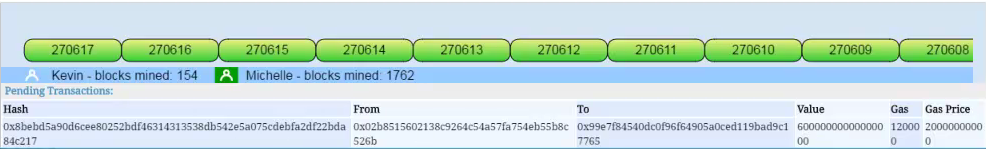
\includegraphics[width=0.69\columnwidth]{blockchain_dapp}
  \caption{Blockchain transaction.}
        \label{fig:abc}
\end{figure}

Mined (confirmed) blocks are represented by the numbered green ovals, unconfirmed blocks will appear as red. 
There is a transaction hash, and the two hashes representing sender (From) and receiver (To). 
Once the block has been successfully mined it will be added to the list of courses pending. One additional exchange (separate from the transactions that pay for enrollment in the course) facilitates its delivery to the course dashboard of the user.
On the current environment this process is instantaneous, on a larger network, e.g. the web-scale Bitcoin blockchain, as currently implemented, to confirm with certainty might take the amount of time required to process a new block, i.e. not more than 10 minutes. Once the course has been completed the administrator can log-on to issue the award. 
After the block containing the award has been mined it can be found in the ``Awards List'' of the associated student. 
% The following code snippet represents a component of an Ethereum ``smart contract'' for an educational institute to offer courses. 
Note that no students are using this course demo for enrolment as it is currently merely a proof of concept.

\begin{figure}[!ht]
  \centering
      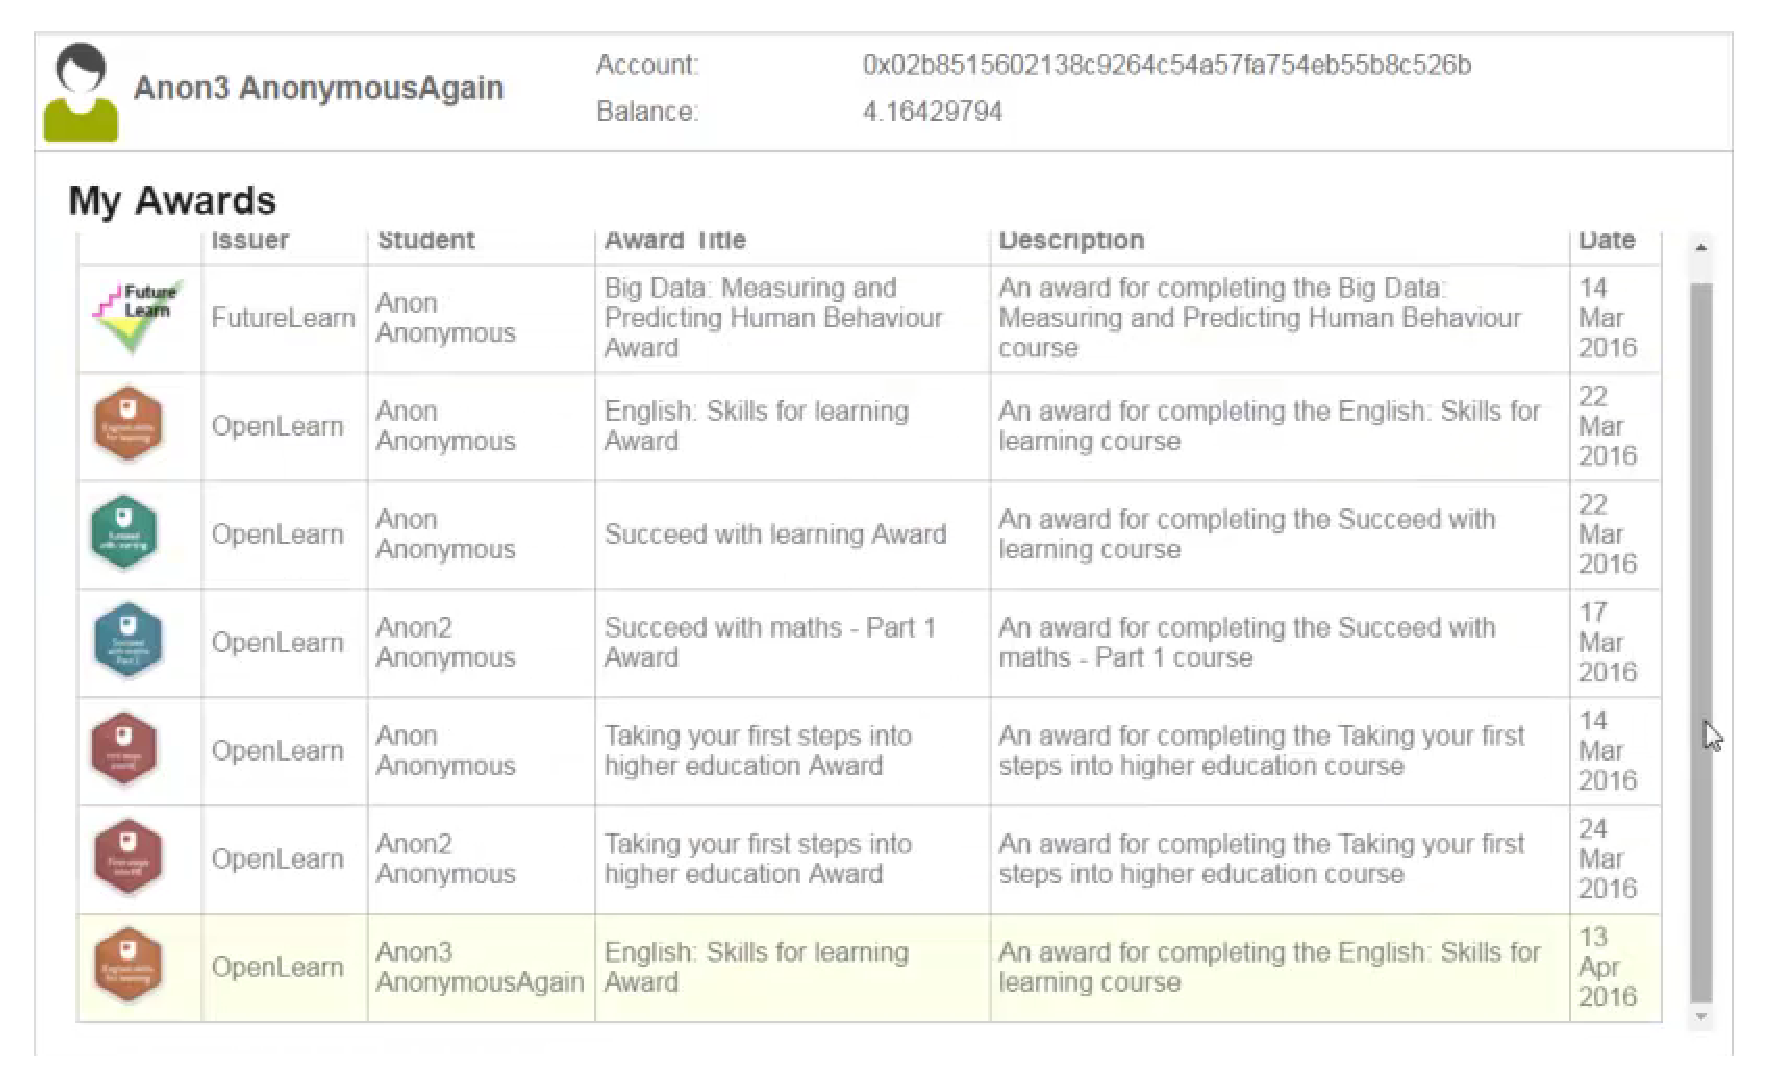
\includegraphics[width=0.69\columnwidth]{awardz}
  \caption{Awards view.}
\end{figure}
\begin{figure}[!ht]
  \centering
\begin{lstlisting}
	function getCourses() public returns
	(address[] availablecourses){
		availablecourses = courses;
		return availablecourses;
	}
	
	function addCourse(address course) 
	public onlyOwner returns (bool success){
		bool exists = false;
		success = false;
		uint i=0;
		uint count = courses.length;
		address next;
		for (i=0; i<count;i++) {
			next = courses[i];
			if (next == course) {
				exists = true;
			}
		}
		if (exists == false) {
			success = true;
			courses.push(course);
		}
	}
\end{lstlisting}
  \caption{Ethereum ``smart contract'' snippet}
\end{figure}
% % \section{Related Work} 

\subsection{Open Badges}

The work we have carried out thus far in the domain of the Semantic Blockchain is largely a continuation of the achievements recorded by the initiatives described in this section. 
The Mozilla Foundation and Peer2Peer University, in collaboration with The MacArthur Foundation, contributed significantly to the field of credential assignment in the context of non-traditional education through the publication of a well known white paper on the subject of modular accreditation~\cite{schmidt2011can}. 
The initiative is known under the name ``Open Badges for Lifelong Learning''.  
The purpose of which is to support skill development and lifelong learning for ``real results'', e.g. job placement and advancement ~\cite{themozillafoundationpeer2peeruniversityincollaborationwiththemacarthurfoundation2011}.

The essence of a digital open badge is a standardized way to conveniently demonstrate that one has achieved a given degree of competency in a particular domain. 
Through close cooperation with credible organizations Open Badges facilitates the process of skill, interest and achievement verification. 
The system is based on an open standard, such that one is free to combine multiple badges from different issuers in a comprehensive accomplishment narrative. 
The aim of this platform is not restricted to the Web and should transcend the digital medium to be applicable to work performed online as well as offline.
Through the shared technical standard Open Badges facilitates a process of garnering recognition for the things one learns as well as the things one is able to teach. 
Anyone who satisfies the standard can award badges. 
There is a vibrant community of contributors and partners supporting this effort, such as NASA, the Smithsonian, Intel, and the American Girl Scouts. 
Originally the badges infrastructure envisioned a decentralized server structure, but the incentives for providers to run these servers were never strong enough to maintain such an environment.
For this reason it appears that the blockchain is a better foundation, as it is run by self-interested entities but can openly be utilized for broad community-based initiatives ~\cite{philippschmidt2015}.

\subsection{Blockchain Certificate Issuance}

We have alluded to the fact that a blockchain database is durable, time-stamped, transparent, and decentralized. 
These characteristics are useful attributes in the management of a reputation system. 
We can consider reputation as a type of currency that enables access to social capital, as opposed to financial capital.
The MIT Media Lab is currently issuing blockchain certificates in accordance with the following procedure:

\begin{enumerate}
\item Create a digital file that contains basic information such as:
\begin{enumerate}
    \item the name of the recipient
    \item the name of the issuer
    \item an issue date
\end{enumerate}
\item Subsequently the contents of the certificates are signed using a private key to which only the Media Lab has access 
\begin{enumerate}
    \item append that signature to the certificate itself
\end{enumerate}
\item Next create a hash, which is a short string that can be used to verify that nobody has tampered with the content of the certificate. 
\item Finally use the private key once again to create a record on the Bitcoin blockchain which states that a certain certificate was issued to a certain person on a certain date
\end{enumerate}

This system makes it possible to verify who a certificate was issued to, by whom, and validate the content of the certificate itself. 
Currently it uses the Bitcoin blockchain by way of the OP\_RETURN field. 
OP\_RETURN is a script operation code used to mark a transaction output as invalid. 
Since the data after OP\_RETURN are irrelevant to Bitcoin payments, arbitrary data can be added into the output after an OP\_RETURN. 
The hash value of the MIT Media Lab is stored in this OP\_RETURN segment.
The current version creates a separate transaction for each certificate.
Future versions of the software could store all hashes in one Merkle tree and only the Merkle root might be stored in the OP\_RETURN, referring back into the blockchain approximately once every day. 

\subsection{Industry Interest}

Sony Global Education, Inc. a division of the multinational conglomerate company Sony Corporation is the foremost industry actor to announce an interest in the adaptation of blockchain technology to the field of education \cite{sonyglobaleducation2016}.
They are pioneering an effort to realize a solution to enable open and secure sharing of academic proficiency and progress records by leveraging the security properties inherent in the blockchain to facilitate the encrypted transmission of data, such as an individual's academic proficiency records and measures of progress, between two specified parties.
Regarding the initiative Sony Global Education has released a public statement to the effect that,

\begin{displayquote}
``\textit{The technology has the potential to realize an entirely new infrastructure system for sharing records securely over the network in any number of ways, opening new doors of possibility for academic records and how they are assessed. For example, after taking an examination to demonstrate his or her academic proficiency level, an individual could direct the testing organization to share the test results with one or more third-party evaluating organizations. This would be a first if implemented on a system-wide basis}''
\end{displayquote}

while notably vague as to the details of the implementation, from this statement we can clearly discern the strong motivation for a solution that under-girds such efforts. 
It enables network users to freely and securely transfer permissions, without the need for an established relationship of trust between network participants, and in such a way that damaging or tampering with programs and data is prohibitively difficult.


\section{Overview}

This chapter represents a first statement on the relationship between blockchains and the Semantic Web, and accordingly we sought to encompass a comprehensive overview that includes all pertinent activity we have thus far undertaken in the space such that it might serve as a catalyst for further development.
We strongly feel that many lessons on how semantics has been aligned with the Web infrastructure could be applied to blockchains. 
The proposed application scenario of MOOCs was selected not for the extraordinary utility that this paradigm provides but to illustrate the concept that the ability to trace an exchange or transaction through the blockchain can provide a social benefit, alleviating the need for holders of credentials to verify their accomplishments ad infinitum, a common problem for those who have obtained degrees abroad.  
Moreover, it seems clear that online learning and the need for new methods to fill existing skills gaps will continue to develop going forward.





    \chapter{Disintermediation of Inter-Blockchain Transactions\label{cha:chapter4}}

Different versions of peer-to-peer electronic cash exist as data represented by separate blockchains. 
Payments between such systems using different ledgers cannot be sent directly from one party to another without going through a financial institution.
Bitcoin's utility is limited to intra-blockchain transactions.
The benefits of peer-to-peer electronic cash are lost if a trusted third party is required to execute \textit{inter}-blockchain transactions.
We propose a solution to the inter-blockchain transaction problem using the same fundamental principles underlying Bitcoin. 
The protocol is described by the \"{U}berledger framework, a hierarchical meta-blockchain layer that encapsulates information regarding the fidelity of peer-to-peer transaction facilitators. 

\section{Introduction}

In the world prior to the introduction of \emph{Bitcoin} no peer-to-peer version of electronic cash had managed to solve the problem of double-spending.  
Nakamoto in \cite{satoshi2008bitcoin} described the state of the art whereby a common solution had been to \enquote{introduce a trusted central authority, or mint, that checks every transaction for double spending... The problem with this solution is that the fate of the entire money system depends on the company running the mint, with every transaction having to go through them, just like a bank}. 

Bitcoin is an effective mechanism to circumvent dependence on a trusted central authority.
However, we have borne witness to the hydralike re-emergence of this phenomenon in the form of exchanges \textit{between} cryptocurrency systems.
For instance to transfer \euro100.00 of value between the cryptocurrencies Bitcoin (BTC) and \emph{Ethereum} (ETH) it is generally necessary to employ the services of an exchange such as \emph{Bitfinex}\footnote{ \texttt{www.bitfinex.com}}.

In this chapter we propose a framework that utilizes the same fundamental principles as Bitcoin.
Bitcoin disintermediates the exchange of value amongst participants on a common blockchain system.
We want to disintermediate transactions between individuals who have accounts on \textit{disjoint} blockchains, but nevertheless want to exchange value with each other. 
In the decentralized constellation of cryptocurrencies the focal points of centripetal force are digital currency exchangers. 
Centralized processes are susceptible to developing into single points of failure, a feature that resilient networks seek to minimize.
Digital currency exchangers provide primarily two services, they transfer value in digital currencies for fiat money, or different digital currencies.
We demonstrate that the interchange of value between different digital currencies is a task that can be performed with high fidelity in the absence of trusted third party exchangers through the use of a hierarchical meta-blockchain layer. 

\begin{figure}
\centering
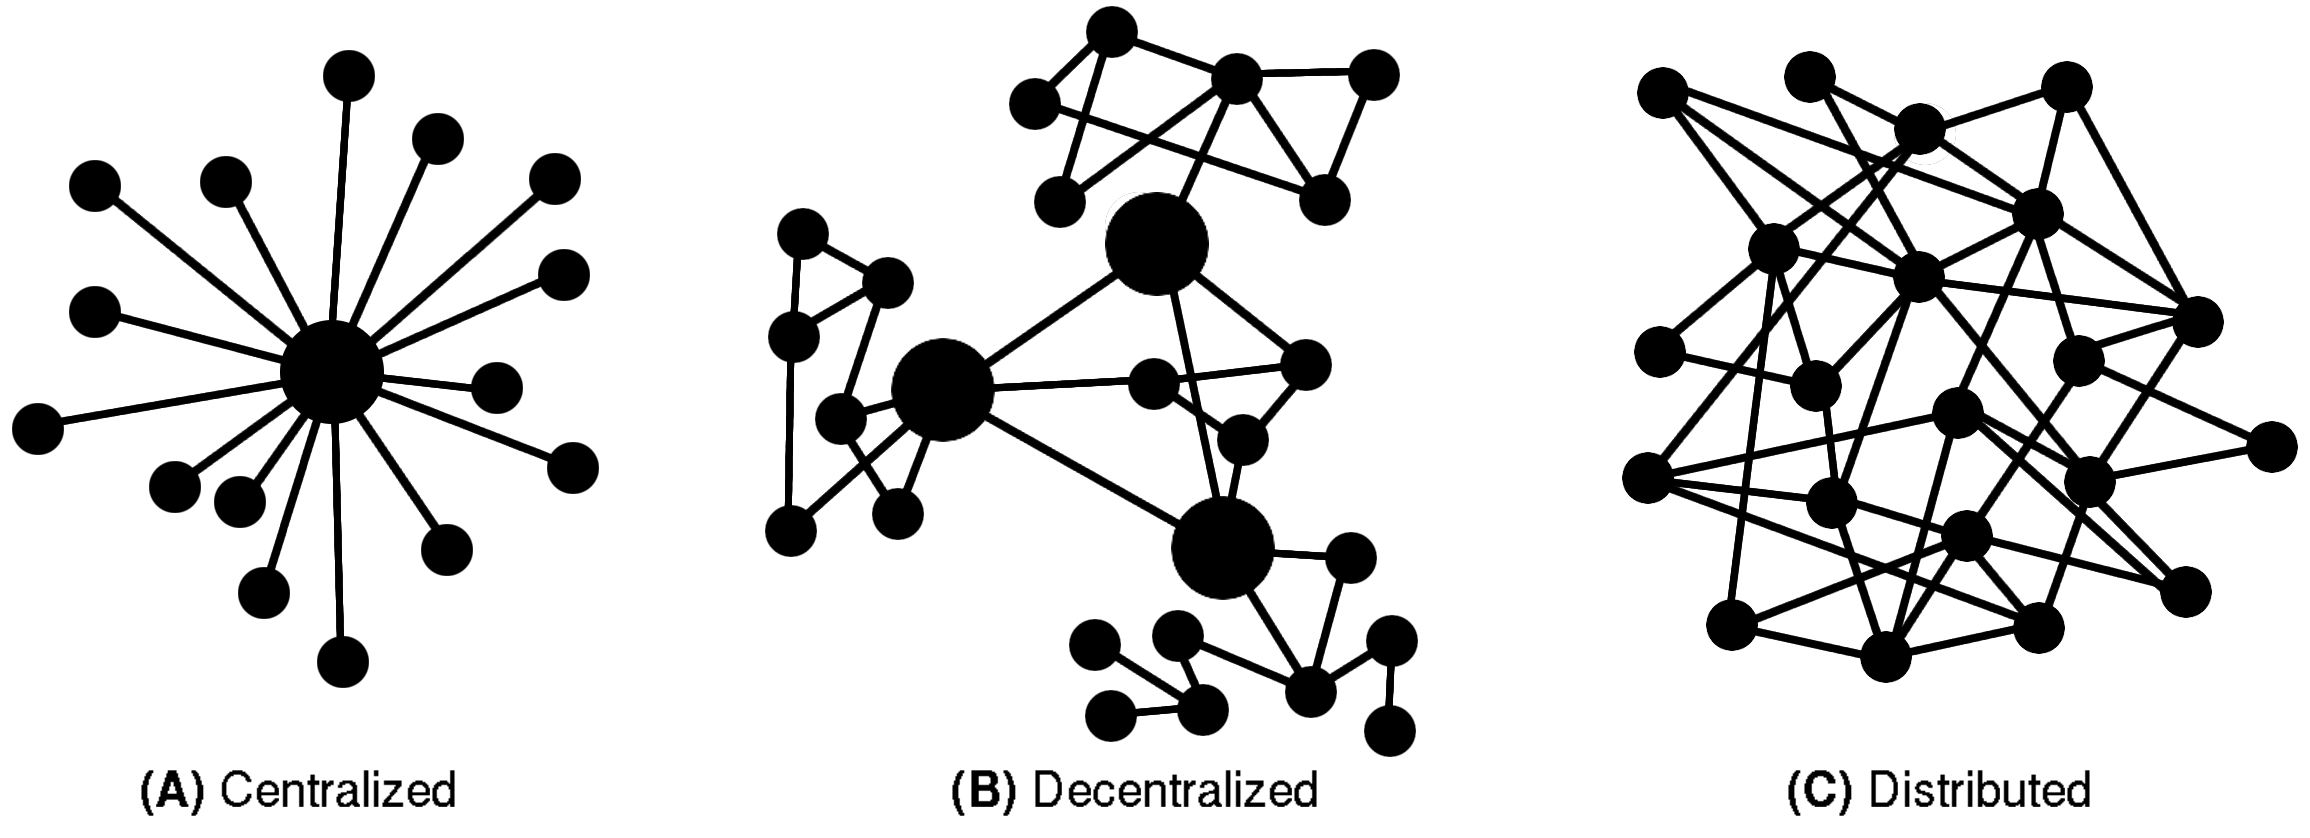
\includegraphics[width=0.5\textwidth]{Figure_1__0}
\caption{Network Topologies}
\end{figure}

\section{The Exchange Model}

On the $2^{nd}$ of August 2016 a highly trafficked digital currency exchange reported a heist of \$72,000,000 USD~\cite{baldwin_2016}. 
This is merely one episode in a history of criminal negligence or malfeasance going back to Mt. Gox (the infamous exchange responsible for the loss of \$460,000,000 in customer funds \cite{wire}) and beyond. 
Accordingly there is a strong interest in viable alternatives to transferring information, viz. value, between disparate blockchain systems independent from such central authorities.

Reliance on exchangers to move value between blockchain systems is a policy that suffers from the \enquote{inherent weaknesses of the trust based model}~\cite{satoshi2008bitcoin}.
Cryptocurrency users who have interacted with an exchange will be familiar with the stringent regime of know your customer (KYC) and will have had direct experience with exchanges \enquote{wary of their customers, hassling them for more information than they would otherwise need}~\cite{satoshi2008bitcoin}. 
As originally envisioned by Nakamoto in \cite{satoshi2008bitcoin} our framework is engineered to \enquote{allow online payments to be sent directly from one party to another without going through a financial institution}.

\begin{figure}
\centering
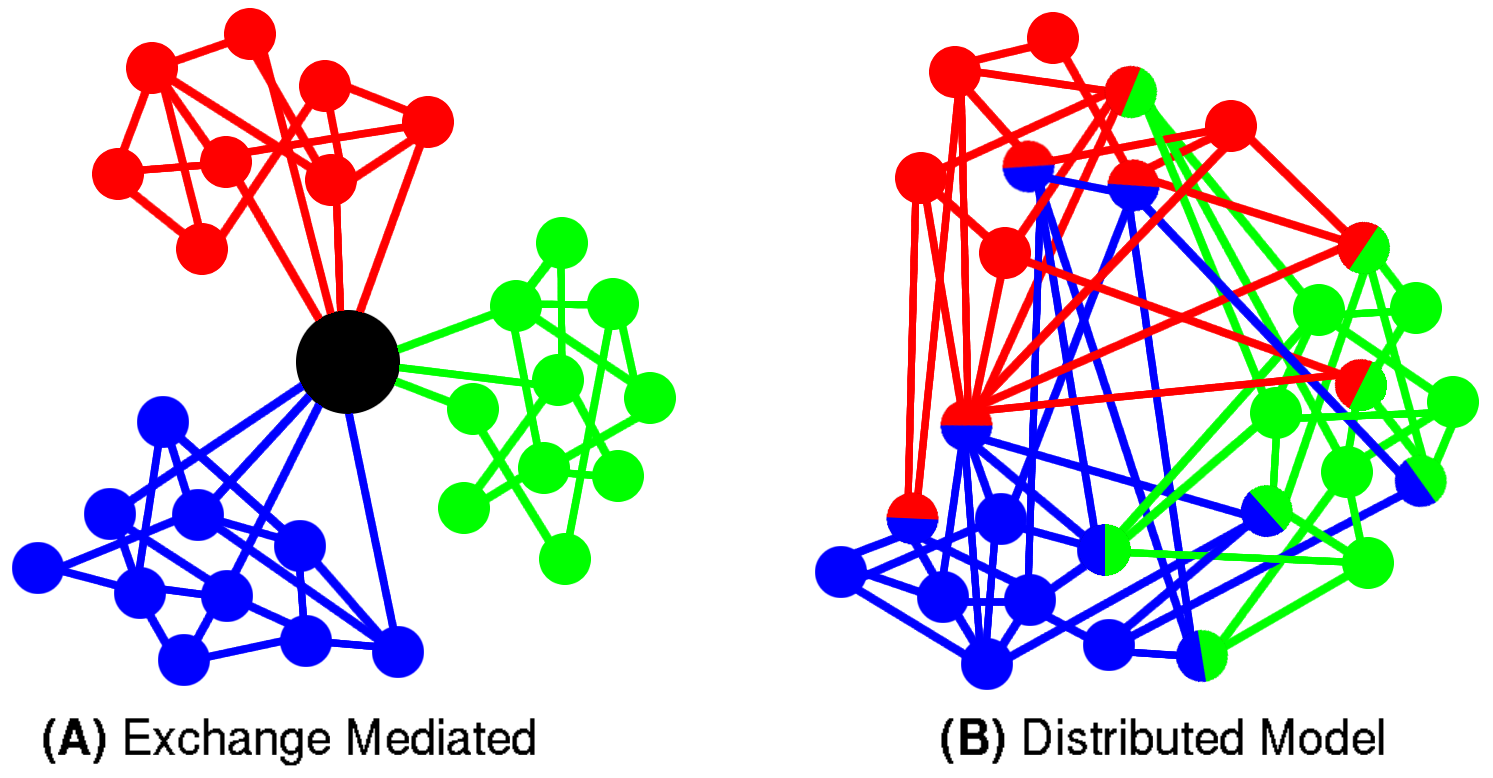
\includegraphics[width=0.5\textwidth]{Figure_2__1}
\caption{Inter-Blockchain Value Transmission}
\end{figure}

\section{Analogous Initiatives}

It has been shown by Thomas \& Schwartz in \cite{hope2016interledger} that protocols whereby a subset of network participants (with accounts on two distinct blockchains) is employed to act as \enquote{connectors and notaries}, i.e. facilitators of a transaction between ledgers, are feasible so long as the subset is sufficiently large to ensure that Byzantine actors can be readily identified ($\mathpzc{n}$ $\geq$ 3$\mathpzc{f}$+1). 

One design feature of the system described in \cite{hope2016interledger} is an ephemeral aggregation of transaction facilitators, such that \enquote{[facilitators] are organized in ad-hoc groups for each payment}.
This arrangement preserves the integrity of the funds involved in the transaction, either they are correctly allocated or the transaction is forfeit.
However information regarding the integrity of each node is not preserved in a publicly available repository of information, such as a blockchain, where it could be put to use in future transactions.  

In contrast to \cite{hope2016interledger} we seek to indelibly preserve all information regarding the successful (or unsuccessful) outcome of the transaction and the behaviour of constituent parties. 
The procedure sketched in Figure 4.3.


\section{Framework Architecture}

We introduce the \"{U}berledger framework\footnote{ \texttt{www.uberledger.io}}. 
It is a hierarchical blockchain model based on the following proposition:  

\theoremstyle{definition}
\begin{definition}{(\"{U}berledger)}
In the transference of value between two disjoint consensus networks the sequentiality of transactions cannot be preserved in the absence of an additional meta consensus network.
\end{definition}

Careful examination of Nakamoto's protocol in \cite{satoshi2008bitcoin} yields a strict sequentiality indicated by timestamps as the crux of the cryptocurrency system. 
We take timestampedness to mean that each transaction ($\mathpzc{t_i}$) is part of a linearly ordered list of transactions ($\mathpzc{T}=(t_1,\dots,t_n)$).
In our model consensus network is equivalent to blockchain, as defined by Kiayias et al. in \cite{garay2015bitcoin}. 

\begin{figure}
\centering
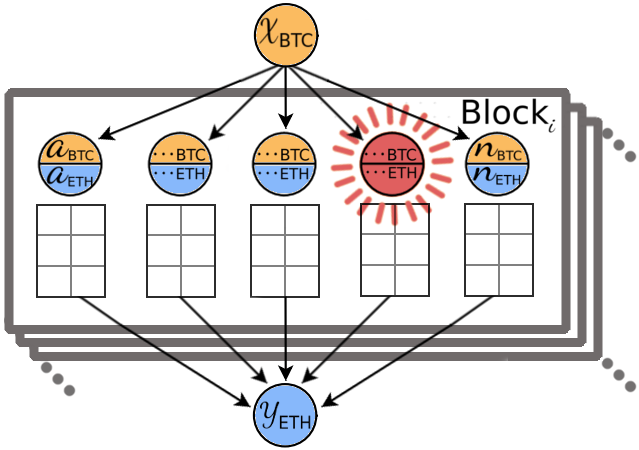
\includegraphics[width=0.5\textwidth]{Figure_3__0}
\caption{Disintermediated Inter-Blockchain Transaction}
\end{figure}

\section{Design Considerations}

\subsection{Incentive Structure}
The incentive structure that motivates the continued maintenance of a resilient blockchain is critical, as the undertaking is costly. 
Honest participants of the \"{U}berledger framework stand to be remunerated in proportion to their ability to attract transaction fees for their services.

\subsection{Data Representation}
Transactions are naturally represented in the form of a 3-tuple ($\mathpzc{P_1}$, $\mathpzc{a}$, $\mathpzc{P_2}$), where $\mathpzc{P_1}$ and $\mathpzc{P_2}$ are the transacting parties and $\mathpzc{a}$ is the article of trade. 
Accordingly, we employ the RDF data model and encapsulate salient transaction information in the form of a graph, as demonstrated in Figure 4. 
To define data in the form of a graph it is necessary to employ a schema.
For this purpose we have adapted the blockchain ontology with dynamic extensibility (BLONDiE)\footnote{\texttt{www.github.com/EIS-Bonn/BLONDiE}}.

This model ensures that a wide range of disparate data resources, e.g. multiple accounts across different blockchains, unique username, reputation information, and cryptographic keys, are rendered in a standardized and universally accessible format adhering to the W3C principles of linked open data.

\subsection{Participant Evaluation}
Insofar as the integrity of nodes in the framework exists as a matter of public record we adapt the design considerations in \cite{kamvar2003eigentrust} to serve as fundamental benchmarks of our peer-to-peer reputation system.
As such the protocol is: 
\begin{enumerate}
  \item Self-policing. 
  \item Anonymity maintaining.
  \item Negatively biased to newcomers.
  \item Minimal in overhead (i.e. computation, infrastructure, storage, and message complexity).
  \item Robust to malicious coordinated collectives.
\end{enumerate}

\section{Results}
The balkanization of the cryptocurrency ecosystem is a phenomenon that is enforced by the business model of the exchanges that seek to exploit their control over channels into and out of different blockchains inhibiting those interested in experimentation on new platforms. Such a climate stifles the ability to assess innovative features and challenge one's understanding of novel techniques. 
Our framework is engineered to redress such toll roads on the highway of creative endeavour.
\"{U}berledger is an open source initiative that seeks to engender an environment of free creative development.

\begin{figure}
\centering
\includegraphics[width=0.5\textwidth]{Facilitator_Graph}
\caption{Transaction Data Model}
\end{figure}


\section{Timestamp Hacking}

Any carnival conjuror can attest that once an audience learns the science behind the way in which a trick is performed, the luster quickly fades. 
The eminent futurist Sir Arthur Charles Clarke is credited with the observation that ``any sufficiently advanced technology is indistinguishable from magic''. 
Of late there is a profusion of hype in circulation about a seemingly magical data structure called a ``Blockchain''. 

Illusionists like Harry Houdini and his ilk can be a great source of entertainment, but when the trick involves a disappearing act on customer confidence, something is amiss. You might have heard that one of the properties a Blockchain possesses is the ability to ``prove certain data exists at a certain moment of time'' or that it somehow ``provides proof that some data existed at a specific tim''. 
The problem with these claims is that they are demonstrably false. 

\subsection*{Look to the Blockchain}

To prove this assertion we need look no further than the publically available Bitcoin Blockchain itself. 
Observe the sequence of blocks, and their associated timestamps, from 145044 to 145048.

\begin{itemize}
\item \texttt{145044: 2011-09-12 15:46:39}
\item \texttt{145045: 2011-09-12 16:05:07}
\item \texttt{145046: 2011-09-12 16:00:05} \\(\textit{Occurs about five minutes before the prior block})
\item \texttt{145047: 2011-09-12 15:53:36} \\(\textit{About seven & about twelve minutes before two prior blocks})
\item \texttt{145048: 2011-09-12 16:04:06} \\(\textit{After two prior blocks but still before} \texttt{145045})
\end{itemize}

We see here that the timestamp of the blocks is not monotonically increasing. 
To understand why, it's necessary for us to have a basic understanding of distributed computing systems, one of the elementary characteristics of which is the lack of a global clock. 
The time adjustment algorithm has even been called the most obvious possible weakness in the Bitcoin protocol.

\subsection*{Why don't the timestamps in the Blockchain always increase?}

It would behove those interested in Blockchain timestamping to consult the Bitcoin wiki for a more informed understanding of how timestamping is applied in this system:

\begin{displayquote}
``A timestamp is accepted as valid if it is greater than the median timestamp of the previous 11 blocks, and less than the network-adjusted time + two hours. `Network-adjusted time' is the median of the timestamps returned by all nodes connected to you.

Whenever a node connects to another node, it gets a UTC timestamp from it, and stores its offset from node-local UTC. The network-adjusted time is then the node-local UTC plus the median offset from all connected nodes. Network time is never adjusted more than 70 minutes from local system time, however''. 
\end{displayquote}

This implies an inherent margin of imprecision. When considering allowances made for anomalies such as daylight savings time and the potential for attacks against the network by malicious actors we quickly see that we need a more nuanced understanding of what timestamping in a Blockchain actually implies. And what it does not.

\subsection*{Timestamp hacking}

One reason that certain parties have an interest in knowingly contributing false timestamps to the network involves the way rewards are distributed according to the Bitcoin protocol. The difficulty of the ``cryptographic puzzle'' that miners are attempting to solve is configured to readjust its difficulty about every two weeks. If miners can fake their timestamps they can make it appear that the network is less powerful than in fact it really is, thus making the puzzle easier and potentially generating higher returns. Additional incentives include denial-of-service attacks against target nodes and in extraordinary cases even double-spend attacks.

\subsection*{Overview}

When one really starts to consider the meaning of time the subject quickly becomes philosophical. 
Spacetime describes a mathematical model that combines space and time into a single interwoven continuum based on the theories of special and general relativity first discovered by Albert Einstein. 
For purposes of time telling in our daily lives we seldom need to grapple with such principles. 
There are some truly impressive applications of blockchain technology. 
For better or worse, precision timestamping is not one of them.


    \chapter{Blockchain-Based Cryptocurrency Network in a Time of Crisis\label{cha:chapter5}}

Blockchain-based cryptocurrencies provide a mechanism for the exchange of value across the internet.
The nature of a public blockchain data-structure is such that a complete record of the transaction history is freely available at all times to all interested parties.
In contrast to traditional econometric approaches this paradigm presents a fundamentally new model for the analysis of dynamic characteristics in a globally distributed network of exchange. 
In this chapter we perform a comprehensive investigation of the distortions and pathologies observable throughout a period of irregular value fluctuation in the transaction network of Bitcoin, a representative cryptocurrency. 
We discover strong structural changes in the dynamical network defined by the transactions between addresses.  
Regions of strong market volatility are characterized by low transitivity in the network. 
Moreover the collapse of the largest financial intermediary and the ensuing crisis this provoked is demonstrated to be clearly discernible solely on the basis of deviations from the Pareto behavior in the degree distribution of the network. 
On the basis of information theory we introduce a new dynamical metric used to quantify volatility fluctuations and measure market anomalies in the network.

\section{Discovered Pathologies}

The global financial crisis of 2008 brought into stark relief the inadequacy of traditional metrics to assess risk. 
This state of affairs can be encapsulated by the headline from January $3^{rd}$ 2009 in the London newspaper The Times which proclaimed \textit{Chancellor on brink of second bailout for banks}.
These words were preserved as a testament to those trying times by their inclusion as a time-stamp in the genesis block of the cryptocurrency Bitcoin (BTC). 
The traditional indicators of economic performance rely on statistics derived through a variety of proxies. 
Economists are hindered in the design of a sound economic policy by scarcity of data.
Specifically what is lacking is a detailed account of all economic transactions. 
The nature of public blockchain-based cryptocurrencies allows for the development of new approaches to perform economic assessment.
In particular, taking account of the full network transaction graph, comprehensive network scientific approaches to the task of quantitatively assessing systemic risk are for the first time realizable in a global medium of economic exchange \cite{battiston2012debtrank}. 
In this chapter we ask, can we assess risk from the meta-data of the blockchain?
In the following sections we utilize the open data proffered by the Bitcoin blockchain to provide a comprehensive assessment of the time period from the $1^{st}$ of October 2013 through the $1^{st}$ of March 2014. 
This period captures the most severe value fluctuations, rapid increase and subsequent crash, since the currency achieved both a modicum of ``mainstream'' recognition and a valuation of 1 BTC to \$100 USD ($1^{st}$ of April 2013). This remains the case through until October $24^{th}$ 2016, the time of writing.  We performed econometric analysis to locate four specific epochs of interest and subsequently defined the network of address transactions to perform network analysis.

In its capacity as a medium of value exchange Bitcoin presents a new model for research into the causes of economic distortions that create risk.
The novelty of the system is predicated on the fact that the complete set of transactions in the Bitcoin ecosystem is recorded by the block-\\
chain, a publicly available information resource.
All BTC exists as divisible and compoundable units assigned to specific addresses indexed in the global list of Unspent Transaction Output (UTXO). 
% The flow of BTC between addresses is preserved in an indelible log which can be viewed freely at all times by all interested parties.
The flow of BTC between addresses is preserved in an indelible public ledger.
Accordingly the blockchain provides a tool for the examination of value exchange between economic actors.
The problem we address in this chapter is whether the structural components of the BTC transaction network can be used to identify conditions of impending market turbulence or risk.
% IS THIS ACCURATE?
We demonstrate this result in the affirmative and go on to present a metric to indicate impending transaction network perturbations. 

\begin{figure}
  \centering
    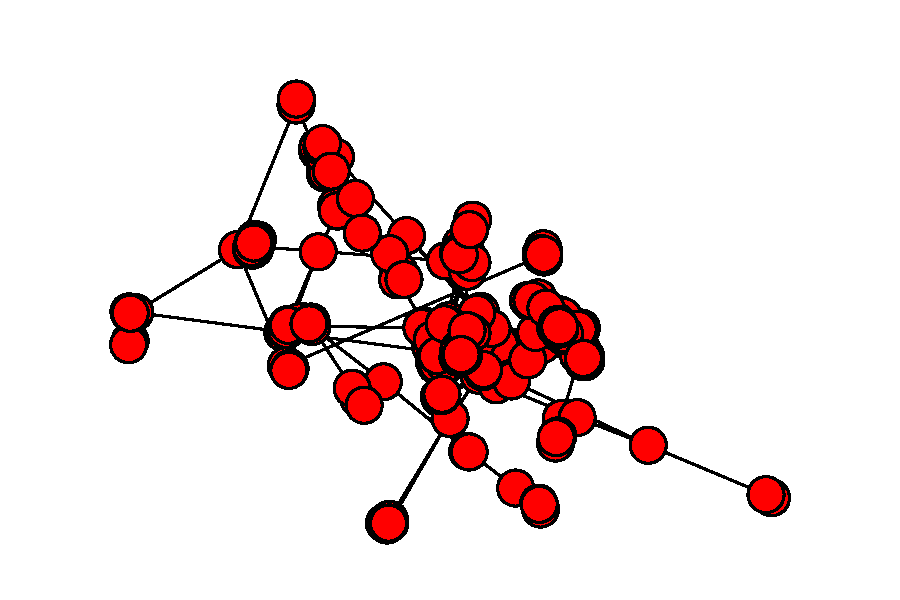
\includegraphics[width=0.5\textwidth]{transactionsNetwork}
  \caption{Maximally Connected Component of Transaction Network: One Hour Prior to Peak Volatility, $8^{th}$ of December 2013}
\end{figure}

\section{Bitcoin \& Blockchain}

Bitcoin is a complex protocol. 
We provide here a brief sketch of the components necessary to understand the analysis presented in this chapter, however due to the many moving parts of the system this is necessarily a superficial overview. 
Interested parties are referred to \cite{narayanan2016bitcoin} for a more complete picture of the system. 

The decentralized currency protocol known as Bitcoin was proposed by Satoshi Nakamoto \cite{nakamoto2008bitcoin}. 
The system utilizes a peer-to-peer (P2P) architecture that enables users to send and receive transactions denominated in units of BTC. 
Users are represented in the network by a public/private key pair. 
Units of BTC can be transmitted to a user by specifying a hash of that user's public key as the receiving party, providing a degree of pseudo-anonymity.  
Users can generate many public keys, i.e. receiving addresses. 
% Secrutiy best practice recommends a new one be used for each transaction. 
The corresponding private keys are used to sign (authorize) transactions. 
Private keys are stored in a ``wallet'' either locally or provided as a hosted service. 

To participate in the Bitcoin network the user runs a client software, such as the Satoshi client, which communicates with a set of peers. 
Transactions are broadcast by the Bitcoin client and received by the peer-to-peer network.
They are confirmed after having been added to the ``blockchain'' - similar to a linked list with the subtle difference that it references the previous block using its hash rather than a pointer. 
This data structure contains blocks of all accepted transactions since the genesis of the system. 

\begin{figure}
\centering
        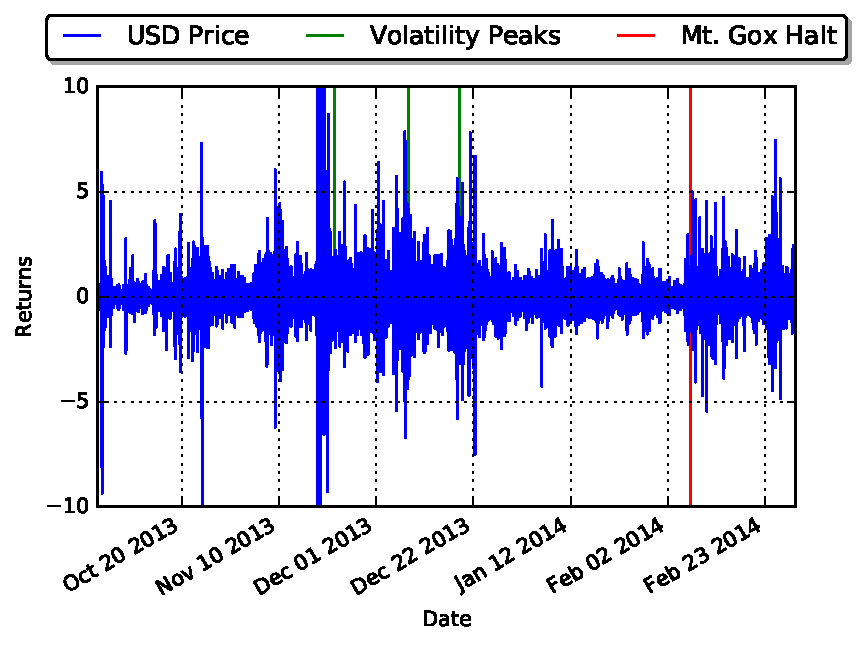
\includegraphics[width=0.6\textwidth]{bitcoinReturns_mtGox}
        \caption{Daily Percentage of Return on Investment}
        \label{fig:RQS}
\end{figure}



Every full node running a Bitcoin client maintains a complete copy of this public blockchain. 
The block generation process confirms new transactions. It necessitates the satisfaction of a computationally expensive ``proof of work'' puzzle. A valid solution to this puzzle entitles the party that deliverers it to the wider network the privilege to issue themselves a reward in the form of newly minted coins. 
The information available through the graph structure of the Bitcoin P2P network is limited due to the dynamic block formation process. 
Each node only has direct knowledge of the peers to which its client is connected. 
The graph of all transactions can be constructed entirely from the publicly available blockchain, wherein the nodes of the graph correspond to Bitcoin addresses and the edges to transactions performed between those addresses. 
In this chapter we empirically study significant global properties of the Bitcoin transaction graph. 

\begin{figure}
\centering
        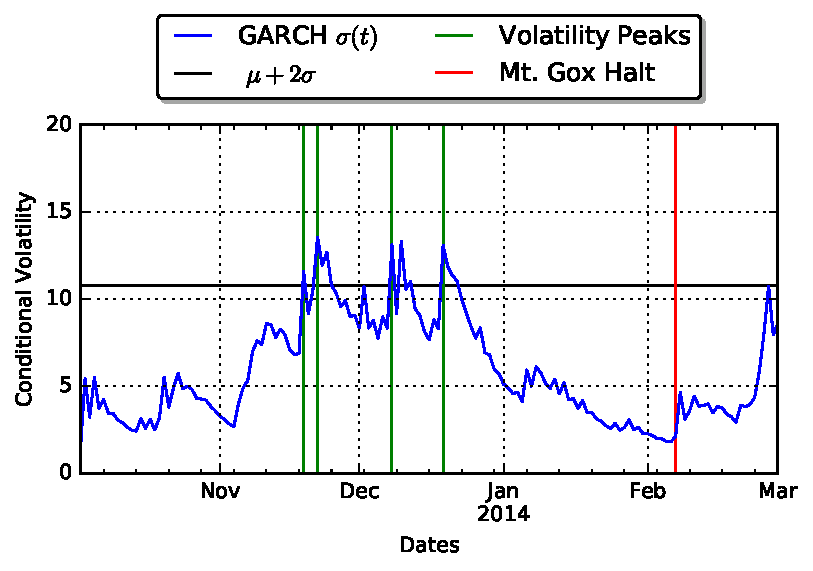
\includegraphics[width=0.8\textwidth]{volatility}
        \caption{Market Volatility}
        \label{fig:PERIODIC}
\end{figure}

\begin{figure}
\centering
        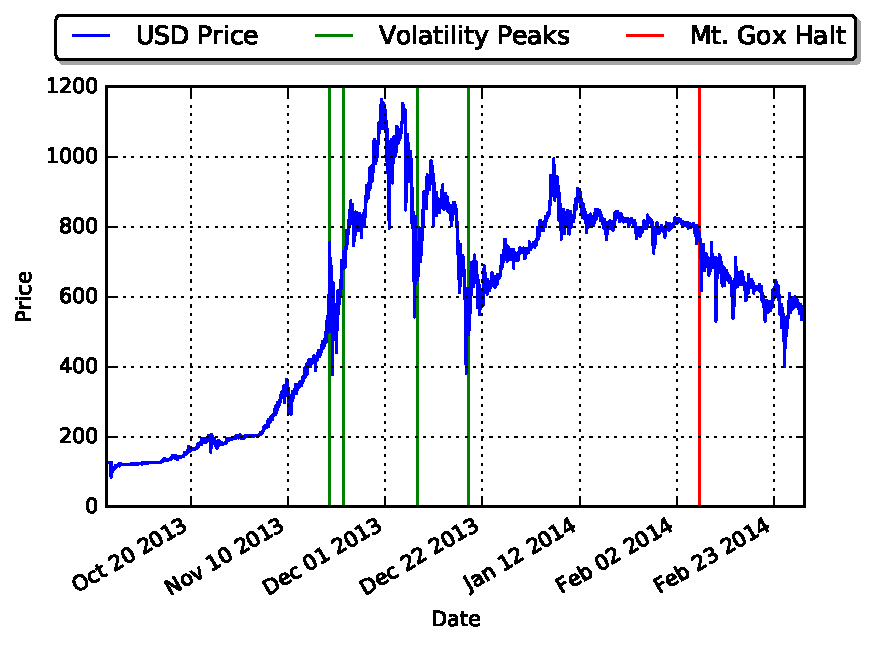
\includegraphics[width=0.8\textwidth]{bitcoinPrice}
        \caption{Bitcoin Price in USD}
        \label{fig:RQL}
\end{figure}
 
With a total market capitalization in excess of \$10,000,000,000 \cite{billy} Bitcoin is the world's largest blockchain-based cryptocurrency. 
The plethora of alternative public blockchain-based cryptocurrencies, many of which are based largely on the open source Bitcoin specification, are amenable to the analyses herein presented.
By a dissection of the full Bitcoin transaction graph throughout four unique phases of exchange activity we discover distinctive characteristics of market pathologies. 

\begin{figure}
\centering
        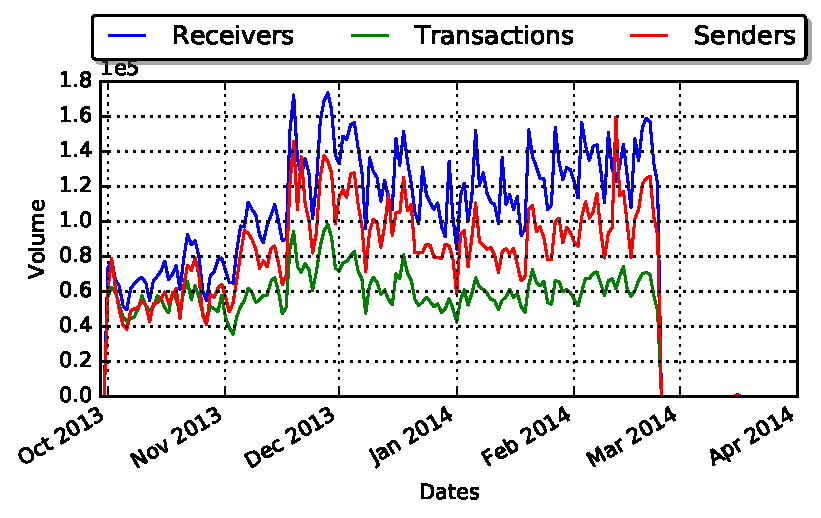
\includegraphics[width=0.6\textwidth]{usersPerDay}
        \caption{Snapshot of Transacting Counter-Parties}
        \label{fig:OU}
\end{figure}

Clustering techniques that associate addresses based on patterns of behaviour degrade the fungibility of individual Bitcoins and in so doing jeopardize the viability of the cryptocurrency as a unit of exchange \cite{moser2014towards}.
As such our work examines addresses on the basis of activity over time, rather than attempting to associate a subset of addresses with a specific identity.
This approach yields insight about network behaviour while preserving the privacy of individual users.

Time series of the USD/BTC exchange rate. We performed a volatility analysis fitting a GARCH model to the returns and established the period of highest market volatitlity through the maximum values of the conditional volatilities as obtained from the model. We show the volume of addresses for both receivers and senders as well as the number of transactions.
% \psfig{file=rosette.ps, height=1in, width=1in,}
Degree distributions for the network of transactions. We can see that the transaction network presents anomalous behavior deviating from Pareto distribution February $5^{th}$ two days before the Mt. Gox transactions halt.

\begin{figure}
  \centering
\begin{lstlisting}[language=json,firstnumber=1]
{
    u'receiver': 
    [  
     {
        u'addr': u'1MZK1SVikQPp2a56cm5q3CPtnwfzNvWyMe', 
        u'value': 17500000000L
     }, 
     {
        u'addr': u'1QJpvMpeuzSoV7nF6u1EVUnDqU7jtBo8Le', 
        u'value': 19980000
     }
    ], 
        u'_id': ObjectId('57fb5ff187a52f69f0ec2802'), 
        u'hash': u'15ccaaaa97790046234e6ef53afcf513cf
        ba2cb1430412b40de544d0fb815a6d', 
        u'senders': 
        [
         {
          u'addr': u'1QJpvMpeuzSoV7nF6u1EVUnDqU7jtBo8Le', 
          u'Value': 19990000
         }, 
         {
          u'addr': u'1CE82aib22UajJ1KtNPTpSH2QKeJZ6o37p',
          u'Value': 17500000000L
         }
        ], 
     u'time': datetime.datetime(2014, 2, 21, 14, 54, 17)
}
\end{lstlisting}
  \caption{Example Data Record}
\end{figure}

\section{Prior Investigations}

The most comprehensive prior treatment of the full (at that time) Bitcoin transaction graph has been conducted by Ron \& Shamir \cite{ron2013quantitative}. 
That analysis considered blocks from January 2009 to May 2012, terminating well before the extreme value fluctuation periods considered in our analysis.
That effort sought to assess statistical properties of the network with a focus on anonymity and the tracking of specific transactions. 
It did not consider structural aspects of the network as a whole as we do in this chapter. 
% Furthermore the time period therein considered terminates well before the extreme value fluctuation periods considered in our analysis. 

Consideration of the Bitcoin transaction network in a time of crisis was undertaken by Donier \& Bouchaud \cite{donier2015markets}, however the data they examine is the order book of Mt. Gox, which was at the time the largest Bitcoin exchange. 
Accordingly, they do not consider the public Bitcoin blockchain data as we do in our treatment. 
Moreover that analysis terminates in January 2014, the month before the collapse of Mt. Gox and the resultant market perturbations that we examine in this chapter. 
The only previous assessment of the Bitcoin bubble of 2013 \cite{garcia2014digital} examines socio-economic signals as opposed to network structure. 
These signals include Twitter data, downloads of the Bitcoin core software client, Google/Wikipedia searches, and prices on various exchanges. 
The work of Ober et. al \cite{ober2013structure} performs an analysis of the transaction graph primarily from the perspective of anonymity and ends before the high volatility periods we examine in this chapter. 
The sole prior work to deal with the crash of Mt. Gox is that of Kristoufek \cite{kristoufek2015main}, which was part of a treatment of the factors that affect the Bitcoin price in terms of speculative activity, considering not blockchain network structure but rather the influence of the Chinese market and technical parameters of the core protocol. 

\begin{figure}
  \centering
    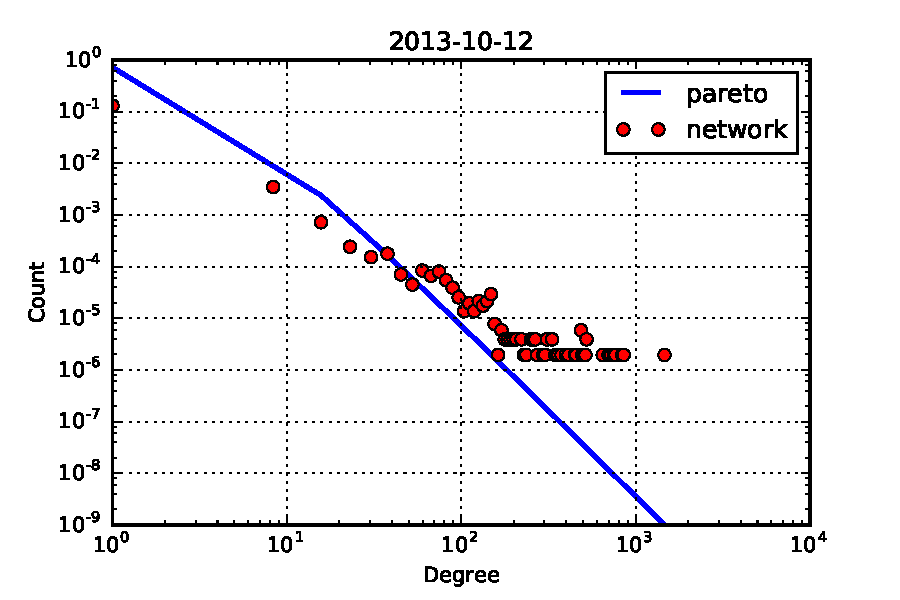
\includegraphics[width=0.8\textwidth]{networkdistribution_2013-10-12_20_30_06.pdf}
  \caption{Normal degree distribution for the network of transactions}
  \label{fig:paretonormal}
\end{figure}

\begin{figure}
  \centering
    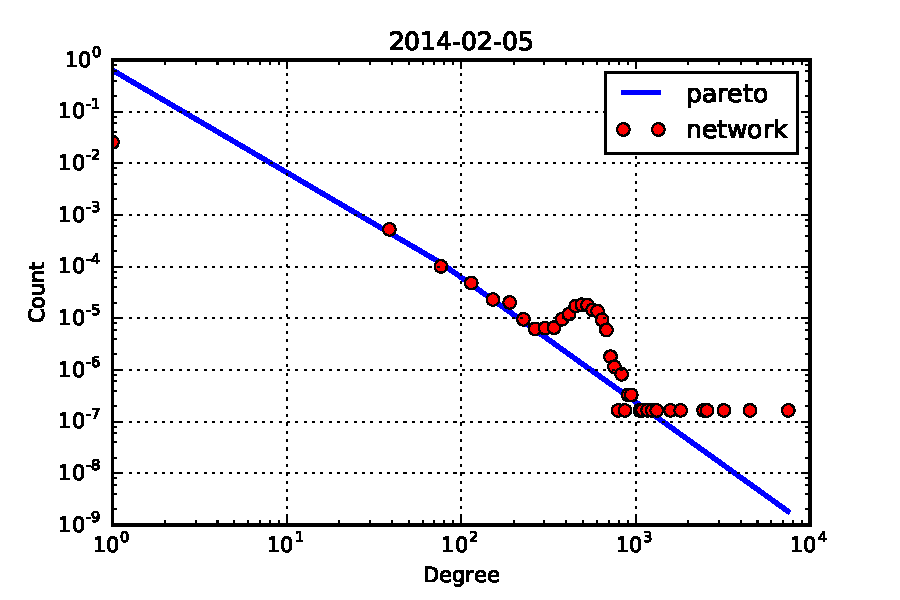
\includegraphics[width=0.8\textwidth]{networkdistribution_2014-02-05_20_30_06.pdf}
  \caption{Mt. Gox degree distribution anomalies}
  \label{fig:anomaly}
\end{figure}

\section{Market Analysis}

% \subsection{Modelling Risk}
In order to characterize the relevant epoch of interest we studied the behavior of the BTC price and performed risk analysis through volatility measures. 
Assessment of risk requires us to define functions of relative uncertainty. 
Volatility catalogs the degree to which the trading price of an asset varies as given by the standard deviation of the return\footnote{Returns here refers to the changes in value of the Bitcoin currency, in our study we use the percent change, or the normalized difference in the prices}. 
Periods of extraordinary market volatility are indicative of high volume fluctuations in nominal value of BTC. We use standard econometric \cite{GARCH} techniques to find the dates of greatest volatility.
Formally, the returns residuals $\epsilon_t$ will be modeled by:

\begin{equation}
\epsilon_t = \sigma_t z_t
\end{equation}

Here $\sigma_t$ represents the standard deviation of the fluctuation at time t and $z_t \sim \mathcal{N}(0,1)$ a noise value at time t, sampled from a normal distribution of mean 0 and variance 1. The index t over $\sigma$ indicates the changes in the fluctuations, $\sigma_t$ is known as the volatility, a measure of the risk in investment, as it quantifies the degree of uncertainty of the future value of the asset. The simplest model for volatility occur in econometrics under the names of ARCH (autoregressive conditional heteroscedasticity) and generalized ARCH (a.k.a GARCH) \cite{GARCH}. Here, heteroscedasticity refers to variations in the fluctuation of the variable of interest, which is in our case $z_t$. Formally, this implies that the covariance $Cov(z_t , z_{t-k})$ depends on time t. The dependence is modeled through past values of the noise $\epsilon_t$ as well as past values of $\sigma_t$.

\begin{equation}
 \sigma^2_t   =  \omega + \sum^{q}_{k=1}\alpha_{k} \epsilon_{t-k}^2 + \sum^{q}_{l=1}\beta_{l} \sigma_{t-l}^2 
\end{equation}

The values of $\alpha_k$, $p$ and $\beta_l$,$q$ determine the correlation of $\sigma_t$ with past fluctuations. For identifying the correct values of the parameters, we fitted the model \footnote{https://pypi.python.org/pypi/arch/3.0} and performed model comparison through Akaike information criteria \cite{Information}.
In generating these models we sought to quantify the degree of market volatility throughout a precisely specified period of time. We show the peaks of high volatility in the Table above.

The highest recorded price of BTC was observed on the $17^{th}$ of November 2013 at \$1,216.73 USD on the exchange Mt. Gox \cite{crash}.
As obtained by volatility analysis we define the \textit{Pre-crash period} and \textit{Post-crash period}, before and after the volatility peak 3.  \textit{Calm period} is given by the first week of January 2014, as it represents stable prices and low fluctuations.
\textit{Pathologies-crash period} on the other hand is given by the first two weeks of February due to volatility and historical knowledge. Mt. Gox halted all Bitcoin withdrawals on the $7^{th}$ of February 2014. Notwithstanding, in each of the other epochs under consideration in our analysis Mt. Gox served as counterparty for the majority of network transactions, at times up to 70\% of all Bitcoin transactions were routed through the platform \cite{wsj}. 


\begin{table}
\centering
\caption{Statistics of Transactions Dataset}
\label{my-label}
\begin{tabular}{|l|c|}
\hline
Sending Addresses:   & 9,951,869  \\ \hline
Receiving Addresses: & 10,447,266 \\ \hline
Total Transactions:  & 8,821,482  \\ \hline
\end{tabular}
\end{table}

In this chapter we take a comprehensive overview of the public blockchain network data.
We examine periods of crisis, such as highly volatile value fluctuations and the implosion of a major financial institution, to discover emergent patterns.  
The epochs considered in this chapter are examined not in terms of classical econometric theory but rather in terms of network structure and empirical analysis. 
The data we use is available as part of the public Bitcoin blockchain as open data.

% \begin{figure}[b]{0.6\textwidth}
%   \centering
%     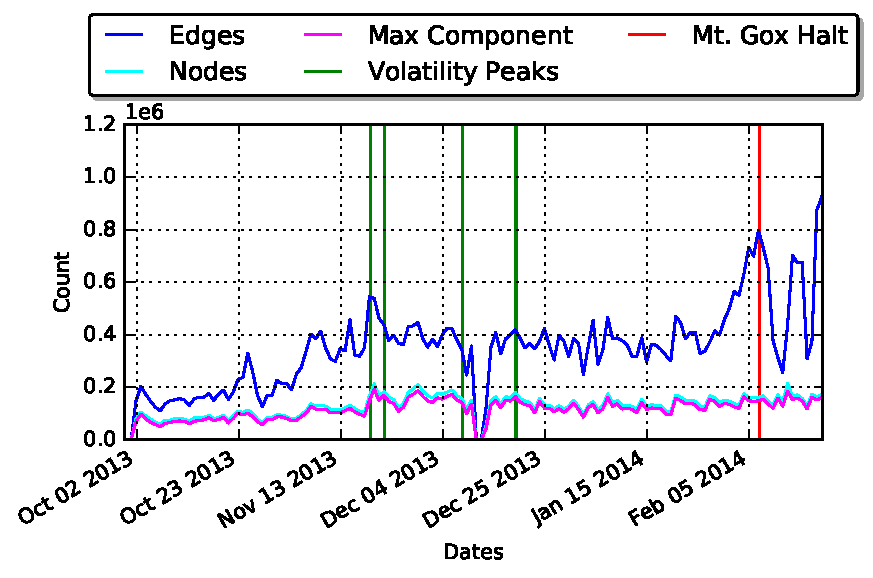
\includegraphics[width=\textwidth]{nodesAndEdges}
%   \caption{Number of Nodes and Edges}
% \end{figure}

% \begin{figure}[b]{0.6\textwidth}
%   \centering
%     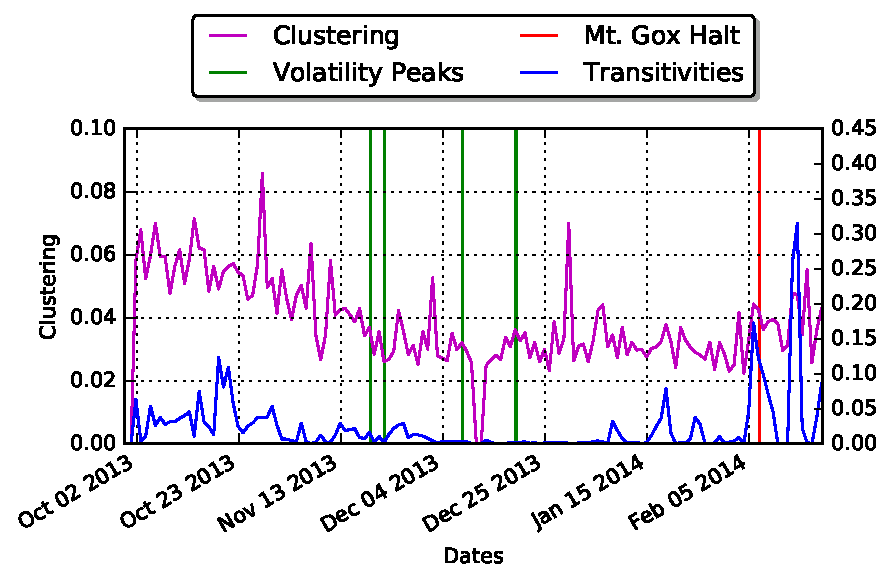
\includegraphics[width=\textwidth]{transitivities}
%   \caption{Transitivities}
%   \label{fig:trans}
% \end{figure}
% Daily values of structural properties in the network of transactions.

\section{Experiment Configuration}

For purposes of our analysis the behavior of the Bitcoin transaction network is grounded by the exchange value of BTC to USD. 
The term \textit{crisis} is used here to describe a period of time wherein the price of BTC suddenly undergoes large fluctuations of nominal value. 
After extended econometric analysis in the above section. We have identified four distinct epochs that portray the Bitcoin transaction network under various conditions of relative stability cataloged in Table 1: Measurement Periods. 

The epochs are labeled according to defining characteristics. \textit{Pre-Crash} is a period of ``irrational exuberance'', that witnessed a general trend towards higher and higher prices. \textit{Post-Crash} entails a precipitous decline in nominal value. \textit{Calm} presents the network under conditions of comparably minor variation in nominal value. \textit{Pathologies-Crash} occurs amidst the implosion of the Mt. Gox exchange, at the time the largest and most central counterparty in the Bitcoin transaction network. We access 28,819 blocks from the Bitcoin blockchain, specifically Block \\ \#260989 of October $1^{st}$ 2013 to Block \#289808 on March $10^{th}$ 2014. From each individual block we extract the transactions. Of each transaction we strip away all data other than the list of inputs and the addresses therein, the list of outputs and the corresponding addresses, and the \texttt{nLockTime}, i.e. the unix time or block number (block height) specifying when the transaction can be accepted into a block. 


\begin{table}
\centering
\label{dates}
\begin{tabular}{|l|c|}
\hline
\multicolumn{2}{|c|}{\textbf{Important Dates}} \\ \hline
\textit{Volatility Peak 1}    & 19 Nov. 2013   \\ \hline
\textit{Volatility Peak 2}    & 22 Nov. 2013   \\ \hline
\textit{Volatility Peak 3}    & 08 Dec. 2013   \\ \hline
\textit{Volatility Peak 4}    & 19 Dec. 2013   \\ \hline
\textit{Mt. Gox Halt}         & 7 Feb. 2014    \\ \hline
\end{tabular}
\end{table} 


The total number of transactions in this set is 8,821,482. We make a distinction between sending addresses, of which there are 9,951,869 and receiving addresses of which there are 10,447,266. This is logically consistent with our expectations due to the concept of a ``change address'' whereby remaining UTXO outputs are assigned to the private key responsible for generating the transaction, thus ensuring that there are typically a higher percentage of receivers in the network than senders. 

% OOOOOOOOOOOOOOOOOOOOOOOOOOOOOOOOOOOOOOOOOOOOOOO
% ooooooooooooooooooooooooooooooooooooooooooooooo
% -----------------------------------------------
% Our network structure analysis was conducted using ASK CESAR WHAT WE USED!

% -basic pareto information

% -explaining the network analysis stuf in high level terms






\begin{table}
\centering
\caption{Measurement Periods}
\label{table:my-label}
\begin{tabular}{|l|c|c|}
\hline
\textbf{Epoch Name:}            & \multicolumn{1}{l|}{\textbf{Begin:}} & \multicolumn{1}{l|}{\textbf{Terminate:}} \\ \hline
\textit{Pre-Crash}         & $1^{st}$ Nov. 2013                          & $6^{th}$ Dec. 2013                              \\ \hline
\textit{Post-Crash}        & $8^{th}$ Dec. 2013                          & $28^{th}$ Dec. 2013                             \\ \hline
\textit{Calm}              & $15^{th}$ Jan. 2014                         & $31^{st}$ Jan. 2014                             \\ \hline
\textit{Pathologies-Crash} & $1^{st}$ Feb. 2014                          & $15^{th}$ Feb. 2014                             \\ \hline
\end{tabular}
\end{table}






% Times of economic panics and crises are exaserbated by uncertainty and lack of confidence. 
% The transparency inherent in blockchain-based cryptocurrencies presents a model whereby access to a complete picture of the transaction network exposed via APIs. 
% It has been said that data is a new natural resource.
% These transactions are one important part of thwarting economic crises the other indispensible component is sophisticated analytical tools. 
% To create an index of market instability we access the information associated with the most severe economic crisis in the history of the Bitcoin currency. 

% For this purpose we accessed 28,819 blocks from the Bitcoin blockchain, specifically Block \#260989 of October $1^{st}$ 2013 to Block \#289808 on March $10^{th}$ 2014. 
% These blocks were further partitioned into four distinct Measurement Periods or epochs that encapsulate particular network structures describing unique configurations of market conditions. 

% The total number of transactions in this set is 8,821,482.
% We make a distinction between sending addresses, of which there are 9,951,869 and receiving addresses of which there are 10,447,266.
% This is logically consistent with our expectations due to the concept of a change address whereby remaining UTXO outputs are reassigned to the private key responsible for generating the transaction. 
% Thus ensuring that there are typically a higher percentage of receiving parties in the network than senders. 

% The term crisis is used here to describe a situation wherein the price of BTC suddenly loses a large percentage of nominal value. 

% data record
% The Bitcoin blockchain encodes transactions together with significant meta-data. 
% For our purposes this was pruned to extract only information applicable to our analysis, as demonstrated by Figure 3.


\section{Economic Distortions}


The Bitcoin network supports a wide variety of market activity.
Small time market participants, less than 50 transactions in the epochs described by our dataset, were excluded from the analysis of the market pathology. 
Accordingly those results are applicable to market actors that receive and transmit a relatively high number of transactions on a consistent basis.
Representative examples of these players include the following: 
\begin{itemize}
  \item Online gambling platforms such as \texttt{SatoshiDice}\footnote{\texttt{http://www.satoshidice.com}} which provide entertainment.
  \item Media outlets including \texttt{CoinTelegraph}\footnote{\texttt{http://www.cointelegraph.com}} that compensate journalists using BTC.  
  \item Darknet markets accessible over the Tor network such as \texttt{AlphaBay Market}\footnote{\texttt{http://pwoah7foa6au2pul.onion}}, providing an auction and corresponding reputation system. 
  \item Purveyors of financial instruments, e.g. binary options purchasable through \texttt{BTC Oracle}\footnote{\texttt{http://www.btcoracle.com}}.
  \item Exchanges including \texttt{Kraken}\footnote{\texttt{http://www.kraken.com}} that serve as a bridge between the fiat economies (USD, EUR, etc.), and as a platform for exchanging between alternative cryptocurrencies such as Litecoin. 
\end{itemize}

In order to gain insight into the mechanism which induced the network distortion we performed an exhaustive analysis of the dynamical patterns for each individual address, and for each characteristic epoch as defined in relevant Table.  
We define a dynamical vector as the hourly departure, i.e. transmission of BTC, volumes for each address.

In order to avoid the curse of dimensionality and uncover relevant dynamical characteristics, we performed dimensionality reduction of the vector matrices through PCA decomposition. 
We subsequently cluster the points with the k-means algorithm. 
The results are presented in the Figure for each of the epochs.

% \begin{figure}
%   \centering
%     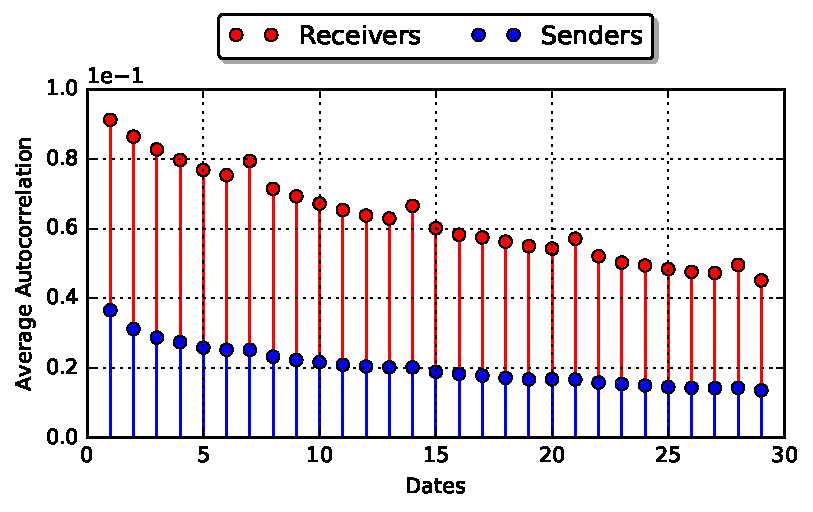
\includegraphics[width=0.3\textwidth]{usersAutoCorrelations}
%   \caption{Auto correlation function of the addresses}
%   \label{fig:auto}
% \end{figure}

% \begin{figure}
%   \centering
%     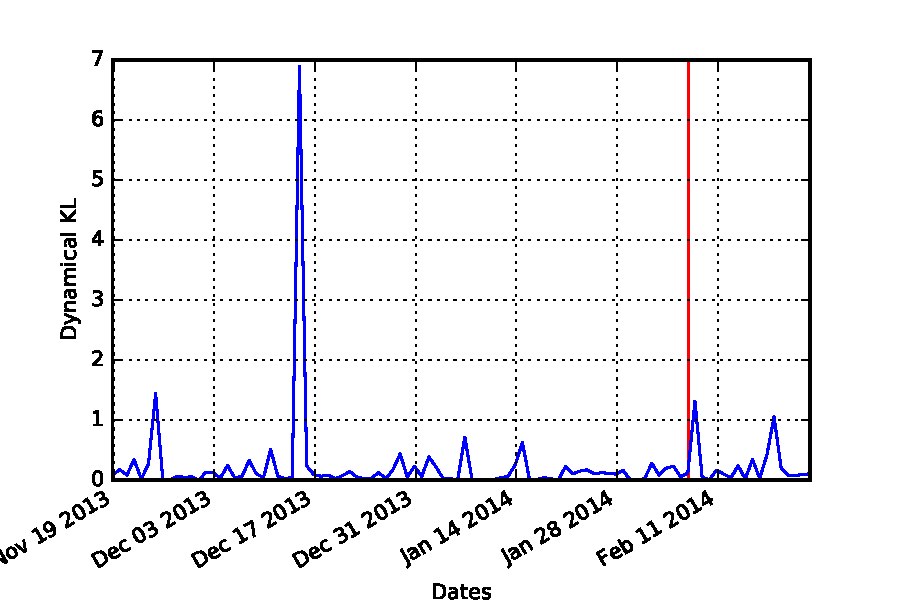
\includegraphics[width=0.3\textwidth]{KL.pdf}
%   \caption{DiscoPath metric for the time period studied. The biggest peaks represent the volatility regions and the Mt. Gox anomalies as pointed out by the red line}
% \end{figure}


The \textit{Pre-crash period} is described by three primary clusters of activity.
The largest of which is represented by a relatively sparse dispersion of departure points.
In contrast the two complimentary clusters of the \textit{Pre-crash period} both feature high volumes of departures that occur with short inter-departure times.
The epoch denoted \textit{Post-crash period} features only two clusters, indicating that the more dense cluster (Red circle), clearly discernible in the other epochs, has been fully absorbed. 
The largest cluster has markedly changed from a sparse dispersion of departures to one punctuated by a 10-fold increase in frequency.
This indicates a waiting period of less duration between transactions.
The decrease in latency between transmission executions is indicative of the variation in the return residual. 
\textit{Pathologies-crash period} corresponds to the long-tail anomaly of Figure 4b. 
We observe in the green cluster an atypically high concentration of send activity over the course of only two days, recall that this is the depiction of a cluster representative i.e. the associated cluster points share the same activity pattern, though not necessarily at the same moment in time. 
This indicates that the cluster point is transmitting BTC to many different addresses in a short time frame. 
The result is high degree connectivity among nodes in the network, induced dynamically. 
This process generates a bifurcation in the cluster structure, in contrast to the ``\textit{stretched}'' structure of the other epochs. 
The \textit{Calm period} is similar in composition to that of the \textit{Pre-crash period}, as it has three distinct clusters and is characterized by relative uniformity in the transmission profile of the cluster representatives.

We seek to define reliable metrics which capture the underlying nature of the meta-data we are analyzing. 
As revealed by the empirical analysis in our description of economic distortions we seek to incorporate both the dynamical as well as the structural component of the observed phenomena. 
We do so by focusing our attention on the unexpected changes in the degree distribution of the daily network of transactions $P_i(k)$. 
The key principle underlying our approach is that, as observed, periods of market distortions are characterized by changes in the \textit{baseline} Pareto distribution.
In times of market fluctuations or anomalies,  the observed distributions $Q_i(k)$ posses a markedly different distribution shape. 

A common approach used to study differences between two distribution $P$ and $Q$ is through the Kullback Leibler divergence  KL(P||Q) \footnote{Referred to also as the relative entropy or the information divergence.}  \cite{Information}.
Intuitively we can understand this distribution as encoding the likelihood that  $P$  produced data from itself, as opposed to the likelihood that it is produced by $Q$ \cite{sloppiness}. 
To incorporate the dynamical aspect, we study the delayed divergence. 
Finally we have:

\begin{equation}
KL(P_{i-1}(k) || Q_i(k)) = \sum_{j}P_{i-1}(k_j)\log{\frac{P_{i-1}(k_j)}{Q_i(k_j)}}
\end{equation}

We call this  metric the ``\textit{DiscoPath}'' (Figure 4b). This formulation possesses several advantages. 
One of which is the encapsulation of the dynamical locality in the sense that we are measuring against the one day delay pattern \textit{baseline} Pareto distribution. 
We would expect a different definition of what the \textit{baseline} is as the market evolves. 
The parameter configuration of a single day delay allows us to uncover both the start and the end of the pathology. 
As the network drifts back to a more typical structural distribution there will be a ``jump''  indicative of the anomaly.

\section{Reflection}

The primary contribution of this chapter is the definition of a metric to recognize perturbations in the transaction networks of public blockchain-based cryptocurrencies such as Bitcoin. 
We performed standard econometric analysis in order to classify different epochs of the blockchain history. 
Further we study basic behavior of the addresses through the autocorrelation function, we then introduced undirected networks upon which we performed network theory analysis.
We found distinctive behavior in the clustering and transitivity of the network, with low values for highly volatile periods and high values after the Mt. Gox crisis. 
After observing the deviations in Pareto behavior, we defined a information theory metric in order to quantify and follow such deviations.

In the time since the epochs examined herein the Bitcoin network has stabilized considerably. 
The network does however remain fraught with smaller scale ``micro-crashes'' and future extensions to our system entail an enhancement of appreciable time scale granularity to facilitate the application of our network to predict more common market anomalies. 
These results are part of an ongoing program of research.
Planned extensions to the work presented include enrichment with geographic information, as well as the definition of a weighted network through the application of transaction amounts to edges between nodes.

Blockchain-based cryptocurrencies on the model of Bitcoin maintain a publicly available record of all the transactions conducted on the network. 
This represents a fundamentally new way of organizing the so-called ``back-end'' processes of a web-scale service. 
The information thus recorded is available to anyone with the interest to examine it, without the strictures of an API limit or a restrictive licensing agreement.
Cryptocurrencies are the first application to fully embrace this model. 
If other web-scale services, such as large search engines or micro-blogging platforms, were to follow suit and organize around a similar model of open data it holds the potential to herald a renaissance in the field of network analytics.  

The Bitcoin model first emerged in the midst of the greatest financial crisis weathered by the traditional economy in living memory. 
The science fiction author William Gibson remarked that ``\textit{when you want to know how things really work, study them when they're coming apart}''.
Accordingly in this analysis we study the Bitcoin network amidst its own time of coming apart, the great bubble of 2013 and the spectacular dissolution of Mt. Gox, the largest and most central financial institution. 
From this time of turbulence we have extracted DiscoPath, a mechanism for the discovering of pathologies, i.e. significant deviations from the typical Pareto distribution of BTC to addresses.
By these means we seek to recognize the manifestation of similar crises in the days, weeks, months, and years to come.

% In this analysis the Bitcoin blockchain afforded us the opportunity to carry-out an exhaustive post-mortem on one of the most severe financial crises to befall this nascent cryptocurency.
% Economists have heretofore endeavored to employ ever more creative mechanisms to infer the behavior of economic actors within a monetary system. 
% The Bitcoin blockchain puts the raw information of value exchange at the fingertips of any and all interested parties. 
% This work represents an initial endeavor into the realm of rigorous network scientific inference of economic principles from an operational cryptocurrency based on a Bitcoin-esque (viz. blockchain) data-structure.




    \chapter{Industry Application Scenarios}

Bitcoin is an emergent phenomenon realized through the subtle interaction of multiple data structures and incentive mechanisms. 
In isolation the various components that comprise the Bitcoin protocol are well known and in some cases have existed for years.
The novelty of Bitcoin was to combine these elements in a previously unimagined way. 
The success of Bitcoin as a cryptocurrency has generated interest in the design principles employed to realize the system.
This in turn has prompted some to critically reassess traditional methods used to process information. 
The purpose being to determine the extent to which architectural aspects of Bitcoin might be replicated in analogous scenarios to reduce or eliminate current inefficiencies. 

\section{Supply-Chain} 

The concept of blockchain, as described by Figure 1.2, is only one aspect of the Bitcoin mechanics that present compelling properties to enterprise information technology engineers.
In this section we describe a small subset of the properties that facilitate useful industry application, especially in the service of supply chain management systems. 

\subsection*{Related Work} 

There are two ``smart contract'' based projects attempting to realize the goal of ameliorating supply chain management through the development of a ``blockchain'' data structure. 
One such operation, known as Provenance states explicitly in the first paragraph of their technical whitepaper ``\textit{the Decentralized Application (Dapp) proposed in this paper is still in development}''.
Another organization under the name of Skuchain does not exhibit a dedicated technical whitepaper describing how their proposed system would work. 
Distinct from these \textit{high level ideas} of how ``blockchain'' technology could be applied towards the improvement of supply chain management, in this section we detail several concrete recommendations. 

\subsection{Data-Structures \& Design Principles}

We highlight a number of fundamental design principles, and where relevant their associated data-structures or cryptographic properties, present in the design of Bitcoin and propose a mapping for how these aspects might be usefully employed in the design of an operational supply chain management system. 

\begin{figure}
  \centering
    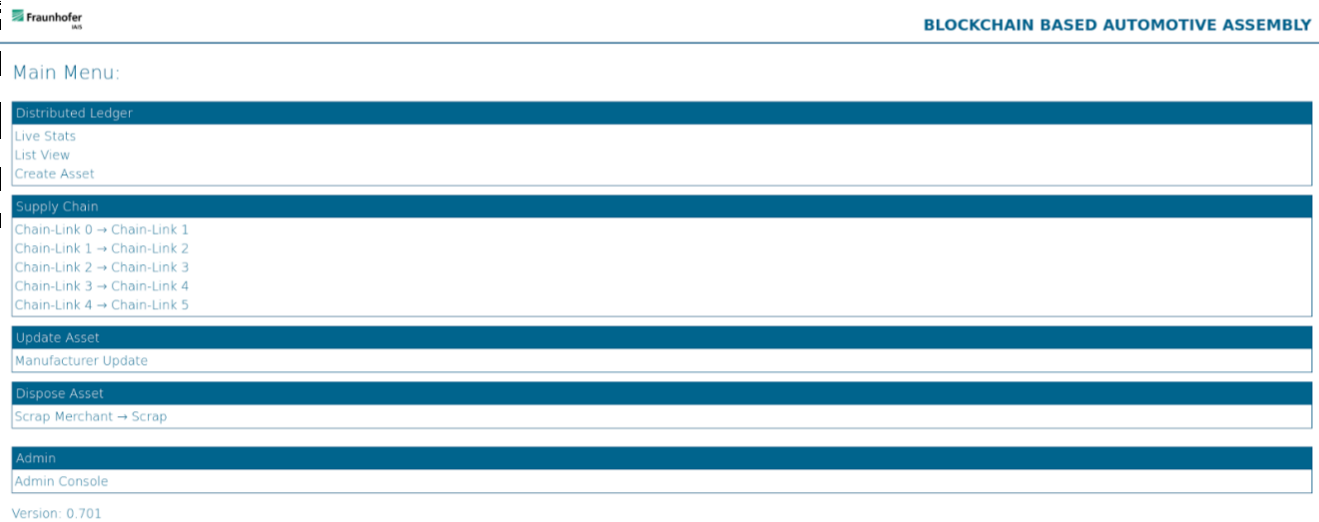
\includegraphics[width=0.8\textwidth]{go0}
  \caption{Main Administrator Dashboard}
\end{figure}

\subsubsection{Pseudo-Anonymity}

This characteristic is one of the fundamental tenants of the ``cypherpunk'' movement that gave rise to the concept of cryptocurency.
Furthermore, practical fungability of individual Bitcoins is important to the viability of this technology as a medium of exchange. 
Association with nefarious activity such as coins that have been involved in deep web market drug deals, such as those that regularly take place on AlphaBay Market, would be subject to confiscation by authorities were they to be positively identified. 
What makes cryptocurrencies attractive to these users in the first place is the property of pseudo-anonymity. 
Network participants are represented only by their address, which if used in accordance with best security practices can be very difficult to associate with a real-world identity. 

These practices employed by $21^{st}$ century drug dealers stand in stark contrast to the techniques employeed in the 1980's, such as those demonstrated in the 2001 movie Blow.
This film also serves to portray a critical aspect of supply chains. 
When the American cocaine importer George Jung introduces his ``Columbian connection'', Diego Delgado, to the head of his distribution network Derek Foreal they are quick to extricate Jung from the process, to his great dismay. 
This brief anecdote serves to underscore the importance of supply chain nodes not being able to identify nodes to whom they are not directly connected, lest they use that resource to ``cut out'' the middleman. 
Representing nodes in a supply chain in such a way that we are able to trace the goods they move through the network while preventing them from de-anonymizing one another is a critical component to a functional supply chain system. 
The pseudo-anamity properties of the Bitcoin network can be usefully applied to the creation of a shared data structure with these constraints. 

% https://en.wikipedia.org/wiki/Replication_(computing)
\subsubsection{Replicated Database}

The idea of using a replicated database to prevent against the corruption of information resources is a well-worn advantageous approach. 
Replication in computing involves sharing information so as to ensure consistency between redundant resources, such as software or hardware components, to improve reliability, fault-tolerance, or accessibility.
Recently this approach has been employed with success by the ``big data'' framework Apache Hadoop among others. 
Bitcoin likewise utilizes this approach by storing a full copy of the blockchain on each network node. 
In a supply chain management system infused with elements inspired by the Bitcoin design the inclusion of the data replication paradigm is important to ensuring that all stakeholders can maintain and independently verify their own copy of the flow of goods or merchandise components. 

\begin{figure}
  \centering
    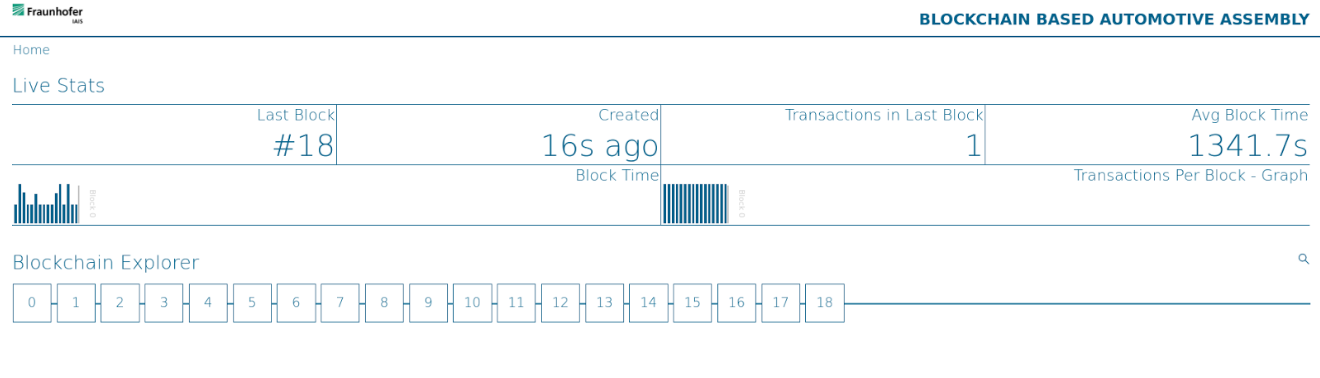
\includegraphics[width=0.8\textwidth]{go1}
  \caption{Blockchain Data Exploration Terminal}
\end{figure}

\subsubsection{Distributed Consensus}

This is a concept closely related to the above section. 
The consensus model in the simplest sense would operate as a mutual agreement between contracting parties and it would take signed acknowledgement of both parties to certify a transaction (or perhaps some other ``proof-of-work'').
Ensuring that the replicated data-sets in each node can form an agreement on a common history.
This process allows different organizations with competing interests to agree on a consistent record.

\subsubsection{Provenance of Data}

To spend a Bitcoin requires that its provenance be explicitly verified against the entire transaction history of the network. 
This feature is beneficial to supply chain systems concerned with targeted recall of defective products, especially so since each individual Bitcoin exists as a unit within the system and cannot be merely \texttt{Crtl + v, Ctrl + v}'d into existence, enforcing uniqueness. 

Targeted recall of products effected by particular components is an important concern to many organizations, for instance large automotive manufacturers. 
In 2015 the Volkswagen emissions scandal (VW-Abgasaff{\"a}re) prompted a vast recall campaign of large subsets of vehicles. 
The problem of tracking vehicle components through the inherent ``mixing'' process that goes on through a supply chain, from material aggregation to finished production is analogous to tracking ``tainted'' coins through the Bitcoin network. 

\subsubsection{Proof-of-Work}

The Bitcoin proof-of-work exhausts computation resources, and ultimately electricity (among other considerations, i.e. the raw materials used to fashion hardware components) in the expending of a scare resource, the money used to buy it, in order to bring new Bitcoins into existence. 
There are alternative models to proof-of-work, one of which is proof-of-stake, even CAPTCHAs could be thought of as a kind of proof-of-work spending, typically, the limited resource of advanced (ideally human-level) visual processing skills. 
Another scarce resource is reputation.
The envisaged system would employ this resource through the reputation associated with an individual private key signature, for a transaction to be committed it would necessitate a signature by both transaction parties, i.e. the transaction quorum. 

\subsubsection{Threat model}

Counterfeiting is a problem that many brands are worried about.
Disingenuous goods circulate widely on the web, and initiatives such as \texttt{code.moncler.com} by French luxury goods manufacturer Moncler which tries to encourage users to register the QR stitched into their product are attempting to combat this growing trend. 
Such as system as we propose here would assist in the tracking of provenance for all goods. 

Another potential threat is that of simple data-corruption, loss, or human-input error. 
The distributed nature of the data model, together with a pre-arranged ``consensus threshold'' or mutual agreement could serve as a resolution to this issue. 
Thereby we prevent corruption of data by malicious parties or equipment malfunction.


\begin{figure}
  \centering
    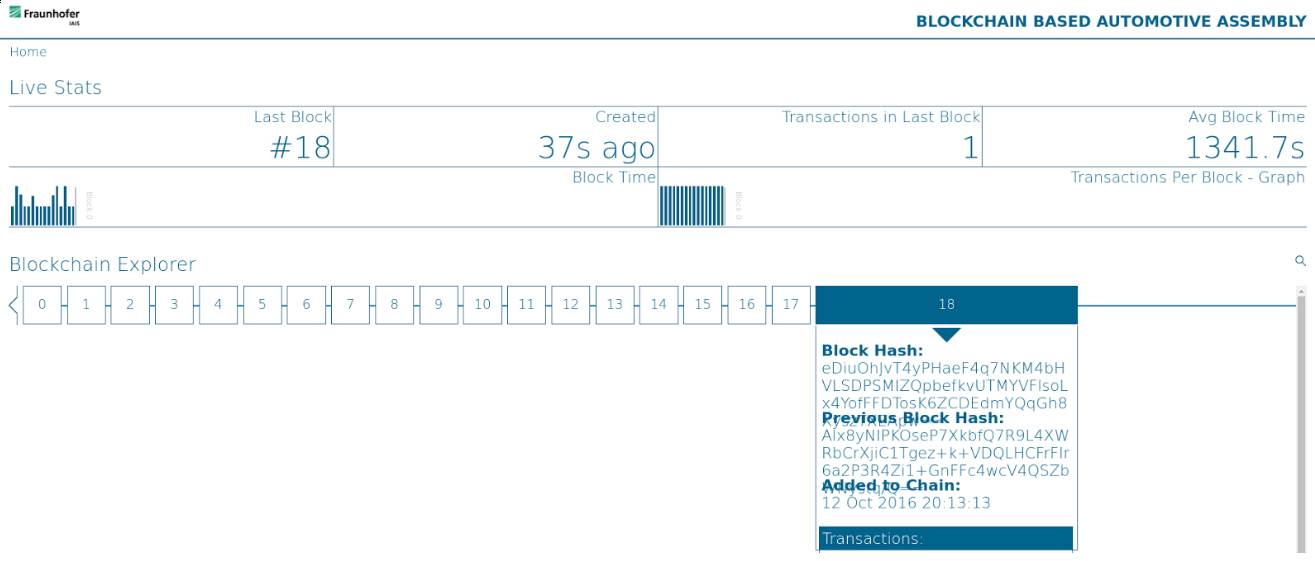
\includegraphics[width=0.9\textwidth]{go2}
  \caption{Transaction Drill-Down}
\end{figure}

\subsubsection{Consortial Blockchain}

This system would be public only among interested parties.
It would spread out emanating from the individual quora of users and gradually could be made extensible to incorporate different components of the network.

\subsection{Demo}

The design framework described in this section was partially realized as an entry in the Hyperledger Blockchain Hackathon of October $3^{rd}$ in Amsterdam for which it was awarded the grand prize in the category of ``outside team''\footnote{http://hollandfintech.com/winner-hyperledger-blockchain-hackathon-announced/}. 


\subsubsection{Discussion}

In \cite{narayanan2016bitcoin} it is pointed out that Satoshi was probably not an academic because he implemented his system first and then wrote about it later, and academics tend to do the opposite. 
This work proves the accuracy of that assertion.
The supply chain management protocol herein described remains to be implemented in code, what this work attempts to do is clearly specify the design of properties that such a system would seek to achieve. 

\begin{figure}
  \centering
    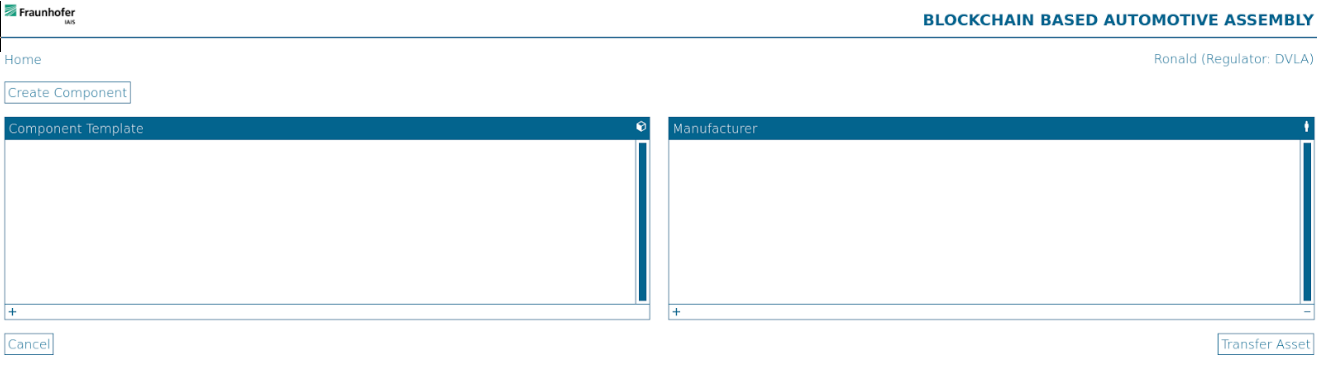
\includegraphics[width=0.9\textwidth]{go3}
  \caption{Primary User Interface Scenario}
\end{figure}
 
\subsection*{Remarks}

In assessing the merits of a technology one is never fully correct and incorrect to prefer one method over another. 
In creating this chapter I might have individually type-set each letter, printed it with ink, and scanned the result into my computer, I chose the more difficult route and used \LaTeX.
Which method is more similar to the use of the designs described above to the complex issues faced in today's long and convoluted supply chains? 
The final determination of the degree to which these techniques are practically useful in the supply chain process is empirical. 
This rough framework and design methodology remains to be validated but nevertheless it is the result of careful consideration on the process whereby one might derive concrete value through the actionable properties of the Bitcoin protocol melded with the real-world problems of a supply chain. 

%%%%%%%%%


% Pseudo-Anonymity

% One of the fundamental tenants of the ``cypherpunk'' movement that gave rise to the concept of cryptocurency

% Fungability remains a primary concern of the Bitcoin core dev community

% Indispensable characteristic of supply chains


% Replicated Database

% In Bitcoin all full nodes retain a complete copy of the database 
% Principle demonstrated to be effective by protocols such as MapReduce 
% Prevents corruption of data by malicious parties or equipment malfunction

% Provenance of Data

% To spend a Bitcoin requires that its provenance be explicitly verified against the entire transaction history of the network 
% Potential benefit to supply chain systems concerned with targeted recall of defective products

% Distributed Consensus

% Ensuring that the replicated datasets in each node can form an agreement on a common history 
% Allows different organizations with competing interests to agree on a consistent record

% Proof of Work

% CAPTCHA 
% Adam Back’s hashcash 
% Proof of stake 
% Private key signatures

% The data structure that supports the cryptocurrency Bitcoin
% Market Cap: \$10,107,045,577 
% Years Operational: 7 
% Number of Addresses: 1.9 million 
% Arguably the world’s only functional blockchain application

% Designing a Data Structure with Properties Similar to Bitcoin’s Data Structure
% Bitcoin and Cryptocurrency Technologies Arvind Narayanan
% “Private blockchain” is just a confusing name for a shared database

\section{Real Estate Property Rights}

Across the Third World, from Honduras to the Republic of Georgia, efforts are underway to establish land titles via the Blockchain. Proponents of this system advocate it as a mechanism to enable marginalized residents of the world's slums to take out loans using this newly recognized property as collateral.

The commodification of people's homes for use as financial instruments was at the heart of the financial crisis of 2008. The correlation between those toxic assets and the Blockchain-based property schemes which are now in the early phases of implementation warrant close scrutiny. Failing to learn the lessons of the last financial meltdown may precipitate another massive disenfranchisement of the world's most vulnerable citizens.

\subsection*{Land Grab Mania}

The financial crisis of 2008 is considered by many economists to have been the worst since the Great Depression of the 1930s. The impetus of this man-made disaster was the securitization of home mortgages which were subsequently arranged into tranches and partitioned on the basis of repayment expectation.

Predatory lenders issued mortgages to unsuspecting victims in the form of NINJA loans (No Income No Job or Assets). These financial instruments were thrust upon people with no real hope of paying them back and the result was countless families losing their homes when the system imploded in 2008.

Hernando de Soto is President of the Institute for Liberty and Democracy. De Soto espouses the notion that residents of Third World shanties such as the Juhu slums of Mumbai, depicted in the film Slumdog Millionaire, are essentially locked out of global capital markets by their inability to secure credit.

\subsection*{Slum property rights}

Officially such people are homeless, lacking governmental title to their domicile. However, the facts on the ground tell a different story. Typically members of these local communities are conscious of one another's de facto property rights, which are acknowledged and respected.

Prior efforts to establish title to such slum properties have resulted in failure as corrupt officials allocated land rights on the basis of favoritism or influence. The Semantic Blockchain presents an appealing alternative as the consensus mechanism might ensure that a majority of residents would act in good faith and correctly assign addresses.

``Of the 7.3 billion people in the world, only 2 billion have a title that is legal, effective and public regarding their control over an asset''. remarked De Soto in a public statement. 
``When something is not legally on record as being owned, it can therefore not be used... as collateral to get credit, as a credential that you can be able to transfer part of your property to invite investment in. Things are owned, but when they're not adequately paperized or recorded, they cannot fill the functions of creating capital and credit''.

\subsection*{Toxic Assets in the Making}

A collateralized debt obligation (CDO) is a type of structured asset-backed security (ABS). 
Originally developed for the corporate debt markets, over time CDOs evolved to encompass the mortgage and mortgage-backed security (MBS) markets. 
In the years leading up to the crash of 2008 some MBS issuers, such as Fannie Mae and Freddie Mac, guaranteed against homeowner default risk while requiring private mortgage insurance on loans in which the borrower provided a down payment of less than 20\% of the property value.

\subsection*{Decentralized insurance}

Together these financial instruments comprised the toxic assets that necessitated the infamous government bailouts which may have been a motivation behind the creation of the world's first digital currency.
Recall that the genesis block of Bitcoin in fact time-stamped itself using the text \textit{The Times 03/Jan/2009 Chancellor on brink of second bailout for banks}.

Peer-to-peer, decentralized, and even autonomous insurance is a concept which is recently gaining traction in the Blockchain community. 
The London Fintech Week Blockchain Hackathon generated a smart contract insurance system which would provide instant compensation on a variety of claims.

In light of pilot projects taking aim at a Blockchain-based land registry currently under way it appears as if a network of mortgage-backed securities generated by first-time borrowers in the Third World might be a near term reality.

It is conceivable that these insurance contracts could, in the foreseeable future, be combined with autonomous smart contract mechanisms to create a DAO (decentralized autonomous organization) of MBS. This has the potential to usher in a new wave of financialization of people's homes.

\subsection*{Learn the lesson of DAO disaster}

Under such a regime repayment tranches could be configured and rated automatically providing more transparency in an industry notoriously opaque to customers and regulators alike.

Lest we fall prey to an epidemic of irrational exuberance we might do well to remember the recent disaster of the DAO and temper our excitement. A system such as the one herein described could unlock vast economic potential, or, to paraphrase Michael Lewis, it could be the making of a new doomsday machine.

Karl Marx noted that ``History repeats itself. First as tragedy, second as farce''. Let us hope that the DAO of the MBS doesn't prove this adage correct.

\section*{Properties of the Blockchain}

On May 22nd, 2010 programmer Laszlo Hanyecz paid 10,000 BTC for two Papa John's pizzas. Today this humorous anecdote is an integral part of the Bitcoin lore, but behind the veneer of playful naivety it masks a more sinister truth. With projects under way in many developing countries to register property, people's homes, on the blockchain are we courting disaster? If a sophisticated programmer is so woefully unaware of the value in such a newfangled digital asset can we expect that a person new to the idea of blockchain, and new to the idea of title itself, can hope to do any better? If the answer is anything less than an unequivocal yes, the consequences will be disastrous.

The idea of registering title, property rights, on the blockchain is touted as a mechanism for fostering social inclusion on a mass scale by the likes of Hernando de Soto, founder and president of the Institute for Liberty & Democracy. De Soto's vision is that by giving people a legal claim over their residence they will have a viable avenue through which they might participate to a greater degree in the larger global economy, for instance by using their home as collateral in a loan application.

Blockchain boasts a consensus mechanism that makes its application in this domain seem very appealing. On one hand, a corrupt government official is likely to allocate property capriciously. However, in a local community, for example in the Brazilian favelas, the local residents should in theory be able to determine democratically who lives where, and based on this majority opinion, aid in establishing a legal claim of ownership. Thus, shanties that have served as individual homes for years and have clear de facto proprietors, but have had no official, viz. governmental, de jure recognition could give their residents immutable claims to ownership.

Title registry in the hands of this newly minted property class has the potential to afford access to vast stores of global capital hitherto unavailable to them, since they had no property to use as collateral. This has the potential to spawn new and previously unimagined economic growth, or conversely to wreak havoc.

In the Republic of Georgia, efforts by De Soto in conjunction with BitFury and Georgia's National Agency of Public Registry (NAPR) are currently implementing a platform for blockchain-based title registration. Papuna Ugrekhelidze, chairman of the NAPR, remarked in a public statement that ``by building a Blockchain-based property registry and taking full advantage of the security provided by the Blockchain technology, the Republic of Georgia can show the world that we are a modern, transparent and corruption-free country that can lead the world in changing the way land titling is done and pave the way to additional prosperity for all''.

Students of history should be aware of the fact that this is not the first time a wave of mass privatization has swept post-soviet countries. Beginning in 1989, a large-scale privatization of formerly state-owned enterprises resulted in the highly inequitable economic topologies of former USSR territories.

One particularly acute example is the case of MMM, a Russian ``company'' that in the 1990s executed what has been called one of the largest Ponzi schemes of all time, defrauding as many as 40 million people to the tune of \$10 billion USD. The case of MMM did not involve title-registration but can be thought of as an historical analogy to illustrate the danger of what might happen when people come into possession of complicated assets that they neither fully appreciate nor comprehend.

Privatization across the crumbling socialist republics often took the form of vouchers, exchangeable for partial ownership of large hitherto state-run institutions, distributed amongst local populations, in places such as the current Republic of Georgia. Scam artists at MMM proved highly adept at convincing unsuspecting proprietors to part with their new and complicated assets for the equivalent of peanuts.  

\subsection*{Bitnation's Experiment in Land Registry}

In the 2008 film Che, Ernesto Guevara states that ``a country that doesn't know how to read and write is easy to deceive''. In the current situation we are likewise talking about literacy, private property literacy and blockchain technology literacy. Educating people in these disciplines will be hard work, but it's nothing that blockchain registry proponents should shy away from; rather, these should become focal points of any efforts going forward.  

``Property literacy'' is a term we understand to mean an appreciation for the system of land registration and ownership as commonly understood through the lense of modern global capitalism. The West African nation of Ghana is a country where ``property literacy'' is not yet pervasive through all levels of society, as indicated by the fact that 70 percent of land lacks proper title.

In keeping with the conceptual framework of De Soto, the organization Bitnation which positions itself as a catalyst to streamline governance processes through the use of blockchain technology, has implemented a blockchain-based land title registration system in Gahna. Founder and CEO, Susanne Tarkowski Tempelhof, explained to Bitcoin Magazine the benefits of these efforts.

``As blockchain applications such as recording and trading physical assets (land, cars, metals etc) emerges in the mainstream, there's a fear of people not understanding the value of the blockchain asset record, and recklessly trading with it, or lending money against it. While this is certainly something to be concerned about during the first years, (probably even decade on the market) I believe it's worth the risk, because the upside is economic empowerment for millions of people, particularly in developing nations with none or weak previous access to create verifiable and immutable ownership records''.

``The ability to seamlessly trade assets like land with each other, and lend money against those assets to finance personal educational or entrepreneurial undertakings will dramatically increase the speed and quality of economic development in frontier and emerging markets, while giving the population a better chance of recourse in case predatory entities such as national governments or local extortion rackets attempt to hijack private property''.

As we endeavour to introduce experimental foreign institutions to people and lands where they are unfamiliar we might also do well to bring them the golden rule of modern capitalism-- ``caveat emptor'' or ``let the buyer beware''. And to those who claim that their efforts will help the disenfranchised of the this earth we offer the message ``primum non nocere'' or ``first, do no harm''.

\section{Electronic Voting}

With the 2016 United States presidential election looming just over the horizon, some of us now turn our thoughts to the process by which American citizens, and indeed all citizens of Democratic countries, make their voices heard as they will in the United States on November $8^{th}$. 
That is, the process by which we cast our votes.

It was stated at the close of the final presidential debate that voting is one of the ``honours and obligations of living in [the United States of America]''.
As citizens, we want to feel that our vote is valuable. 
The question is, do we feel certain in the knowledge that our votes will matter? 
Are our governments doing everything possible to ensure that this is the case?    

\subsection*{2000, Fraud in Florida}

Back in 2000, the contested election between George W. Bush and Al Gore was plunged into a quagmire by the purportedly confusing nature of the ballot that citizens used to cast their votes. This resulted in the Bush v. Gore case that worked it's way up to the Supreme court finally putting an end to the recounting of votes in Florida. 
As a millennial, I have some recollection of the drama that accompanying battle for Florida's electoral votes precipitated.

Having grown up in the age of the personal computer, I can't help but feel the method by which my fellow citizens were asked to register their preference for the leader of the free world is uncomfortably antiquated. Are these arcane conventions, like Congressional rulebook, inextricably entrenched or is it possible for us to do any better?

\subsection*{Close elections}

Another arcane (shall we say \textit{byzantine}?) system of transmitting valuable information is through the Society for Worldwide Interbank Financial Telecommunication (SWIFT) founded in 1973. This juggernaut is in the process of being disrupted by Ripple Labs, one of the world's most innovative, and most successful, Blockchain companies. 
If Semantic Blockchain technology can potentially unseat SWIFT, which as of September 2010, linked more than 9,000 financial institutions in 209 countries, exchanging an average of over 15 million messages per day, is it so implausible to suspect that a Blockchain might be able to disrupt the business model of voting machine manufacturers to bring more accountability to the hallowed task of recording the sentiment of America's 146,311,000 registered voters?

In its most basic form, a Blockchain can be understood as a linked list which utilizes hash pointers to ensure that the record is appended only, that data once written cannot be modified or erased. 
More complex instantiations of Blockchain technology adopt many of the properties of the data structure that facilitates the Bitcoin cryptocurrency.

A data structure with such properties would doubtless have come in handy in the highly contested 1948 Democratic Party primary in the state of Texas. The race that pit the then Congressman Lyndon Baines Johnson and the acting governor Coke Stevenson against one another for the party nomination. The same race wherein Johnson claimed victory by a margin of 87 votes out of 988,295 cast, amidst rampant allegations of voter fraud. It's asserted prominently in the book Means of Ascent (1989) by Robert A. Caro that Johnson stole that election and in so doing, forever changed the course of the American history. The election having set the stage for Johnson to assume the presidency in 1963.

\subsection*{Civic engagement}

The idea of preventing such miscarriages of voter preference by means of electronic voting has already been popularized in the Baltic nation of Estonia, where the 2007 Estonian parliamentary election was implemented by means of internet voting, a worldwide first.

Civic engagement in the United States is not nearly as robust as it could be especially among the millennial generation. 
Blockchain technology has already done much to shake up the global finance industry and inspire passionate young people to engage with the intricacies of payment processing, a hitherto lacklustre subject. 
Blockchain a potential impetus to increased participation in electoral campaigns. 
    \chapter{Conclusion\label{cha:chapter8}}

As is evidenced by Figure 7.1 in 2016 ``blockchain'' is undergoing an intense period of inflated expectations. 
That being the case there \textit{are} indeed practical use cases for this technology dispite the rampant over-speculation.
In this chapter we illustrate this from the perspective of industry, with application to the concept of the ``industrial data space''. 

John Henry is an American folk hero who worked as a ``steel-driving man'', hammering steel to blast away centuries-old rock in the construction of that big iron needle stitching the country together - the US railway system. Legend has it that John Henry's prowess as a steel-driver was measured in a race against a steam-powered hammer, a race he won, only to die in a pyrrhic victory with his hammer in his hand while his heart gave out from stress.
The battle for pre-eminence in the race to deliver the steam hammers of tomorrow is a tale that dates back longer than that of the Mechanical Turk. 
As more and more complicated tasks in the human repertoire yield way to computerized automation perhaps we as a species will have more time to develop our higher cognitive abilities, such as attempting to read the minds of the companies seeking to read (and recreate) our minds!

\section{Industry Impact}

The daring knight sacrifice which shattered the meticulously planned defense kicked off a chain of events that forced a full resignation in fewer than twenty moves. With that, the title of reigning world champion of chess, one of mankind's most vigorous intellectual pursuits, was bestowed on a computer.

In 1972 the World Chess Championship in Reykjav{\'i}k pitted the American Bobby Fischer against the USSR's Boris Spassky in a landmark event of the Cold War confrontation. The fateful day in 1997 when for the first time a computer was able to defeat the incumbent world champion of chess, marked a turning point in what some have labeled a new Cold War, not between world superpowers, but between men and machines.

As there are games within games there are Cold Wars within Cold Wars. Amidst the struggle to outperform humans in the tasks traditionally associated with the highest intellectual rigour there is a struggle for leadership in the determination of who exactly it will be to develop and deploy the latest and greatest of salient machines. To the victor go the spoils and the organization that can successfully pull off these feats can expect to be handsomely rewarded.

The International Business Machines Corporation (IBM) mustered the effort to put the chess champion computer Deep Blue into action and for years they have been at the forefront of the struggle to improve the cognitive ability of machines. 
In 2011 IBM's DeepQA lab spawned Watson, the question answering computer system that trounced former human champions Brad Rutter and Ken Jennings on the quiz show \textit{Jeopardy!}.

\begin{figure}
  \centering
    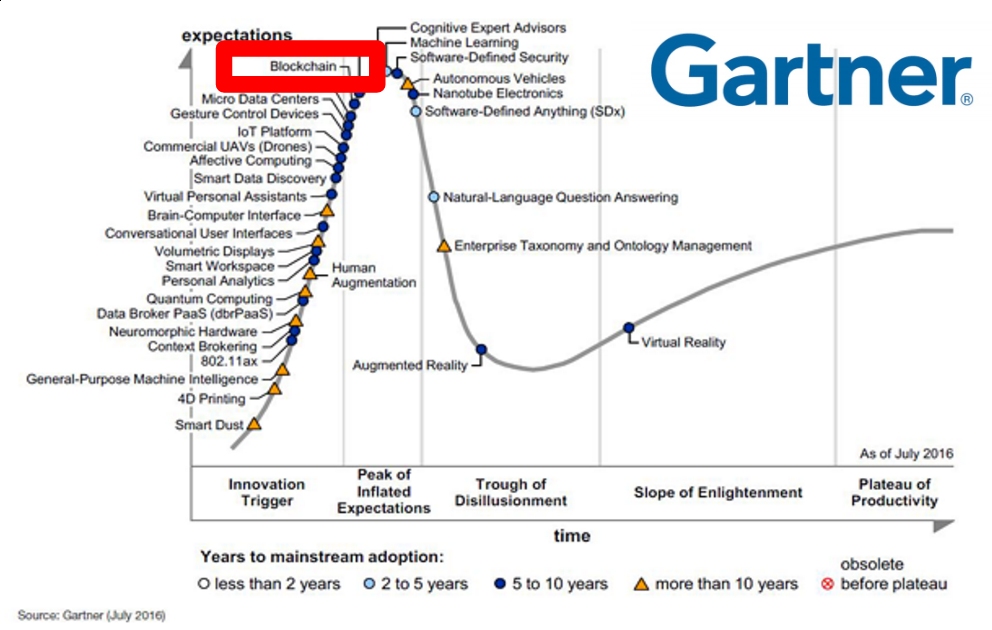
\includegraphics[width=0.75\textwidth]{go4}
  \caption{Gartner's Hype Cycle}
\end{figure}


The Cold War was an arms race. Just as the USSR's launch of Sputnik precipitated a period of frenzied turmoil for NASA, the recent success of Google's AlphaGo has sent shock waves through IBM. AlphaGo is the computer program which beat a professional human Go player, without handicaps on a full-sized 19x19 board in March 2016. As such it represents a serious challenge to IBM's storied supremacy in the race for the machine mind.

\subsection*{Can elephants dance?}

In a recent IBM symposium entitled Emerging Technologies for the Enterprise: Cognitive Computing and Blockchain. How humans and machines are forging a new age of understanding, the role of cognitive computing was described as ``systems that learn at scale, reason with purpose, and interact with humans naturally. Most important, rather than being explicitly programmed, they learn and reason from their interactions with us and from their experiences with their environment. They are made possible by advances in a number of scientific fields over the past half-century, and are different in important ways from the information systems that preceded them. Those systems have been deterministic; cognitive systems are probabilistic. They generate not just answers to numerical problems, but hypotheses, reasoned arguments, and recommendations about more complex -- and meaningful -- bodies of data''.

Fabric, IBM's contribution to the Hyperledger Project, is a Blockchain implementation with a modular architecture allowing pluggable implementations of various functions. It features powerful container technology to host any mainstream language for smart contracts development.

To date, IBMs investments in the realm of the Semantic Blockchain through the Fabric initiative have been substantial. The magnitude of IBM's moves into the space of the Semantic Blockchain portends that they anticipate this technology will play a significant role in their future. As IBM now bills themselves as a leader in the ``Cognitive Computing'' revolution, it is certain that Semantic Blockchain will play a prominent role in the next man vs. machine showdown.

\subsection*{Speak softly and carry a big stick}

The vocal advocacy of IBM in the Blockchain space stands in stark contrast to Google's almost complete silence on the subject. Prussian military theorist Carl Philipp Gottlieb von Clausewitz in his treatise \textit{On War} wrote that ``surprise plays a much greater role in strategy than in tactics'', and of course the famous Sun Tzu is remembered by the words ``when the enemy is close at hand and remains quiet, he is relying on the natural strength of his position''. 
To assume that Google is doing nothing in the Semantic Blockchain space is naive. 
Let us look forward with anticipation, and, for some, perhaps dread, to what eventually Google plans to roll out.

\section{Outlook\label{sec:outlook}}

The keen interest of large industry players in the realm of blockchain technologies has precipitated an initiative by the Linux foundation to standardize components of the so-called blockchain architecture, analogous to the way in which the World Wide Web Consortium (W3C) has endeavoured to standardize aspects of the Semantic Web. 
The effort is known as \textit{Hyperledger} and consists of a loose confederation of IT service providers interested in providing ``blockchain as a service solutions''. 
The most active members at present are IBM and to a lesser extent Intel. 
In general terms it is conceived of as a ``shared database and app engine''. 
As the fundamental exemplar of a private permissioned and consortial blockchain it will be interesting to observe how this project develops going forward. 

As noted previously Ethereum uses money as a proxy (viz. ``hack'') to solve the halting problem.
Since the cost of computation (i.e. gas) is heavily subsidized the network appears to be unsustainable.
Furthermore the community recently split in a ``hard fork'', and it appears that further partitions are imminent. 
Public commitment to migrate towards a ``proof of stake'' mining model also present potential dangers. 

The \textit{Lightning Network} is a private 2-way communication/payment channel and serves and as extension to the Bitcoin network.
This endeavour may present the ability to scale the transaction throughput of the network in a way that is acceptable to all stakeholders, thereby ensuring the long-term viability of system. 
Moreover this project is conceivably a new phase in the evolution of blockchain technology, potentially facilitating applications such as atomic cross-chain transactions.

Pegged Sidechains that utilize the Bitcoin blockchain as an infrastructure backbone upon which other coins and ideas can take shape is likewise indicative of a new direction for the future growth of the cryptocurrency ecosystem. 

\section{Concluding Discussion\label{sec:dissemination}}

With a total market capitalization in excess of \$10,000,000,000, more than 7 years of continued operation, and over 1.9 million addresses Bitcoin is the world's most successful blockchain-based cryptocurrency. 
We argue that it is the world’s \textit{only} long-term viable blockchain application to date. 
This work comprises a comprehensive programme of research undertaken into the nature of the Bitcoin protocol in an effort to assess the degree to which it's fundamental components could be applied to alternative use-cases.
The question we sought to answer was whether the data structures and incentive mechanisms that facilitate Bitcoin could be melded with semantic applications and techniques to realize concrete solutions to practical problems.
Having demonstrated this result in the affirmative we look forward to the continued growth of this burgeoning field of research. 
    % \input{./chapters/chapter8}

% ---------------------------------------------------------------
\backmatter % no page numbering from here
    % \addchap{List of Acronyms}

\begin{tabbing}

\end{tabbing}
\endinput

		
		% if you want to provide a glossary with explanations of important terms put it in here

    \bibliographystyle{geralpha}
    \bibliography{./bib/references}
    
    % \addchap{Annex}

\begin{appendix}



\end{appendix}

\endinput


\end{document}
